
%% bare_jrnl.tex
%% V1.4b
%% 2015/08/26
%% by Michael Shell
%% see http://www.michaelshell.org/
%% for current contact information.
%%
%% This is a skeleton file demonstrating the use of IEEEtran.cls
%% (requires IEEEtran.cls version 1.8b or later) with an IEEE
%% journal paper.
%%
%% Support sites:
%% http://www.michaelshell.org/tex/ieeetran/
%% http://www.ctan.org/pkg/ieeetran
%% and
%% http://www.ieee.org/

%%*************************************************************************
%% Legal Notice:
%% This code is offered as-is without any warranty either expressed or
%% implied; without even the implied warranty of MERCHANTABILITY or
%% FITNESS FOR A PARTICULAR PURPOSE! 
%% User assumes all risk.
%% In no event shall the IEEE or any contributor to this code be liable for
%% any damages or losses, including, but not limited to, incidental,
%% consequential, or any other damages, resulting from the use or misuse
%% of any information contained here.
%%
%% All comments are the opinions of their respective authors and are not
%% necessarily endorsed by the IEEE.
%%
%% This work is distributed under the LaTeX Project Public License (LPPL)
%% ( http://www.latex-project.org/ ) version 1.3, and may be freely used,
%% distributed and modified. A copy of the LPPL, version 1.3, is included
%% in the base LaTeX documentation of all distributions of LaTeX released
%% 2003/12/01 or later.
%% Retain all contribution notices and credits.
%% ** Modified files should be clearly indicated as such, including  **
%% ** renaming them and changing author support contact information. **
%%*************************************************************************


% *** Authors should verify (and, if needed, correct) their LaTeX system  ***
% *** with the testflow diagnostic prior to trusting their LaTeX platform ***
% *** with production work. The IEEE's font choices and paper sizes can   ***
% *** trigger bugs that do not appear when using other class files.       ***                          ***
% The testflow support page is at:
% http://www.michaelshell.org/tex/testflow/



\documentclass[journal]{IEEEtran}
%
% If IEEEtran.cls has not been installed into the LaTeX system files,
% manually specify the path to it like:
% \documentclass[journal]{../sty/IEEEtran}





% Some very useful LaTeX packages include:
% (uncomment the ones you want to load)


% *** MISC UTILITY PACKAGES ***
%
\usepackage{ifpdf}
% Heiko Oberdiek's ifpdf.sty is very useful if you need conditional
% compilation based on whether the output is pdf or dvi.
% usage:
% \ifpdf
%   % pdf code
% \else
%   % dvi code
% \fi
% The latest version of ifpdf.sty can be obtained from:
% http://www.ctan.org/pkg/ifpdf
% Also, note that IEEEtran.cls V1.7 and later provides a builtin
% \ifCLASSINFOpdf conditional that works the same way.
% When switching from latex to pdflatex and vice-versa, the compiler may
% have to be run twice to clear warning/error messages.






% *** CITATION PACKAGES ***
%
%\usepackage{cite}
% cite.sty was written by Donald Arseneau
% V1.6 and later of IEEEtran pre-defines the format of the cite.sty package
% \cite{} output to follow that of the IEEE. Loading the cite package will
% result in citation numbers being automatically sorted and properly
% "compressed/ranged". e.g., [1], [9], [2], [7], [5], [6] without using
% cite.sty will become [1], [2], [5]--[7], [9] using cite.sty. cite.sty's
% \cite will automatically add leading space, if needed. Use cite.sty's
% noadjust option (cite.sty V3.8 and later) if you want to turn this off
% such as if a citation ever needs to be enclosed in parenthesis.
% cite.sty is already installed on most LaTeX systems. Be sure and use
% version 5.0 (2009-03-20) and later if using hyperref.sty.
% The latest version can be obtained at:
% http://www.ctan.org/pkg/cite
% The documentation is contained in the cite.sty file itself.






% *** GRAPHICS RELATED PACKAGES ***
%
\ifCLASSINFOpdf
   \usepackage[pdftex]{graphicx}
  % declare the path(s) where your graphic files are
  % \graphicspath{{../pdf/}{../jpeg/}}
  % and their extensions so you won't have to specify these with
  % every instance of \includegraphics
  % \DeclareGraphicsExtensions{.pdf,.jpeg,.png}
\else
  % or other class option (dvipsone, dvipdf, if not using dvips). graphicx
  % will default to the driver specified in the system graphics.cfg if no
  % driver is specified.
  % \usepackage[dvips]{graphicx}
  % declare the path(s) where your graphic files are
  % \graphicspath{{../eps/}}
  % and their extensions so you won't have to specify these with
  % every instance of \includegraphics
  % \DeclareGraphicsExtensions{.eps}
\fi
% graphicx was written by David Carlisle and Sebastian Rahtz. It is
% required if you want graphics, photos, etc. graphicx.sty is already
% installed on most LaTeX systems. The latest version and documentation
% can be obtained at: 
% http://www.ctan.org/pkg/graphicx
% Another good source of documentation is "Using Imported Graphics in
% LaTeX2e" by Keith Reckdahl which can be found at:
% http://www.ctan.org/pkg/epslatex
%
% latex, and pdflatex in dvi mode, support graphics in encapsulated
% postscript (.eps) format. pdflatex in pdf mode supports graphics
% in .pdf, .jpeg, .png and .mps (metapost) formats. Users should ensure
% that all non-photo figures use a vector format (.eps, .pdf, .mps) and
% not a bitmapped formats (.jpeg, .png). The IEEE frowns on bitmapped formats
% which can result in "jaggedy"/blurry rendering of lines and letters as
% well as large increases in file sizes.
%
% You can find documentation about the pdfTeX application at:
% http://www.tug.org/applications/pdftex





% *** MATH PACKAGES ***
%
\usepackage{amsmath}
% A popular package from the American Mathematical Society that provides
% many useful and powerful commands for dealing with mathematics.
%
% Note that the amsmath package sets \interdisplaylinepenalty to 10000
% thus preventing page breaks from occurring within multiline equations. Use:
%\interdisplaylinepenalty=2500
% after loading amsmath to restore such page breaks as IEEEtran.cls normally
% does. amsmath.sty is already installed on most LaTeX systems. The latest
% version and documentation can be obtained at:
% http://www.ctan.org/pkg/amsmath





% *** SPECIALIZED LIST PACKAGES ***
%
\usepackage{algorithmic}
% algorithmic.sty was written by Peter Williams and Rogerio Brito.
% This package provides an algorithmic environment fo describing algorithms.
% You can use the algorithmic environment in-text or within a figure
% environment to provide for a floating algorithm. Do NOT use the algorithm
% floating environment provided by algorithm.sty (by the same authors) or
% algorithm2e.sty (by Christophe Fiorio) as the IEEE does not use dedicated
% algorithm float types and packages that provide these will not provide
% correct IEEE style captions. The latest version and documentation of
% algorithmic.sty can be obtained at:
% http://www.ctan.org/pkg/algorithms
% Also of interest may be the (relatively newer and more customizable)
% algorithmicx.sty package by Szasz Janos:
% http://www.ctan.org/pkg/algorithmicx




% *** ALIGNMENT PACKAGES ***
%
\usepackage{array}
% Frank Mittelbach's and David Carlisle's array.sty patches and improves
% the standard LaTeX2e array and tabular environments to provide better
% appearance and additional user controls. As the default LaTeX2e table
% generation code is lacking to the point of almost being broken with
% respect to the quality of the end results, all users are strongly
% advised to use an enhanced (at the very least that provided by array.sty)
% set of table tools. array.sty is already installed on most systems. The
% latest version and documentation can be obtained at:
% http://www.ctan.org/pkg/array


% IEEEtran contains the IEEEeqnarray family of commands that can be used to
% generate multiline equations as well as matrices, tables, etc., of high
% quality.




% *** SUBFIGURE PACKAGES ***
%\ifCLASSOPTIONcompsoc
%  \usepackage[caption=false,font=normalsize,labelfont=sf,textfont=sf]{subfig}
%\else
%  \usepackage[caption=false,font=footnotesize]{subfig}
%\fi
% subfig.sty, written by Steven Douglas Cochran, is the modern replacement
% for subfigure.sty, the latter of which is no longer maintained and is
% incompatible with some LaTeX packages including fixltx2e. However,
% subfig.sty requires and automatically loads Axel Sommerfeldt's caption.sty
% which will override IEEEtran.cls' handling of captions and this will result
% in non-IEEE style figure/table captions. To prevent this problem, be sure
% and invoke subfig.sty's "caption=false" package option (available since
% subfig.sty version 1.3, 2005/06/28) as this is will preserve IEEEtran.cls
% handling of captions.
% Note that the Computer Society format requires a larger sans serif font
% than the serif footnote size font used in traditional IEEE formatting
% and thus the need to invoke different subfig.sty package options depending
% on whether compsoc mode has been enabled.
%
% The latest version and documentation of subfig.sty can be obtained at:
% http://www.ctan.org/pkg/subfig




% *** FLOAT PACKAGES ***
%
%\usepackage{fixltx2e}
% fixltx2e, the successor to the earlier fix2col.sty, was written by
% Frank Mittelbach and David Carlisle. This package corrects a few problems
% in the LaTeX2e kernel, the most notable of which is that in current
% LaTeX2e releases, the ordering of single and double column floats is not
% guaranteed to be preserved. Thus, an unpatched LaTeX2e can allow a
% single column figure to be placed prior to an earlier double column
% figure.
% Be aware that LaTeX2e kernels dated 2015 and later have fixltx2e.sty's
% corrections already built into the system in which case a warning will
% be issued if an attempt is made to load fixltx2e.sty as it is no longer
% needed.
% The latest version and documentation can be found at:
% http://www.ctan.org/pkg/fixltx2e


%\usepackage{stfloats}
% stfloats.sty was written by Sigitas Tolusis. This package gives LaTeX2e
% the ability to do double column floats at the bottom of the page as well
% as the top. (e.g., "\begin{figure*}[!b]" is not normally possible in
% LaTeX2e). It also provides a command:
%\fnbelowfloat
% to enable the placement of footnotes below bottom floats (the standard
% LaTeX2e kernel puts them above bottom floats). This is an invasive package
% which rewrites many portions of the LaTeX2e float routines. It may not work
% with other packages that modify the LaTeX2e float routines. The latest
% version and documentation can be obtained at:
% http://www.ctan.org/pkg/stfloats
% Do not use the stfloats baselinefloat ability as the IEEE does not allow
% \baselineskip to stretch. Authors submitting work to the IEEE should note
% that the IEEE rarely uses double column equations and that authors should try
% to avoid such use. Do not be tempted to use the cuted.sty or midfloat.sty
% packages (also by Sigitas Tolusis) as the IEEE does not format its papers in
% such ways.
% Do not attempt to use stfloats with fixltx2e as they are incompatible.
% Instead, use Morten Hogholm'a dblfloatfix which combines the features
% of both fixltx2e and stfloats:
%
% \usepackage{dblfloatfix}
% The latest version can be found at:
% http://www.ctan.org/pkg/dblfloatfix




%\ifCLASSOPTIONcaptionsoff
%  \usepackage[nomarkers]{endfloat}
% \let\MYoriglatexcaption\caption
% \renewcommand{\caption}[2][\relax]{\MYoriglatexcaption[#2]{#2}}
%\fi
% endfloat.sty was written by James Darrell McCauley, Jeff Goldberg and 
% Axel Sommerfeldt. This package may be useful when used in conjunction with 
% IEEEtran.cls'  captionsoff option. Some IEEE journals/societies require that
% submissions have lists of figures/tables at the end of the paper and that
% figures/tables without any captions are placed on a page by themselves at
% the end of the document. If needed, the draftcls IEEEtran class option or
% \CLASSINPUTbaselinestretch interface can be used to increase the line
% spacing as well. Be sure and use the nomarkers option of endfloat to
% prevent endfloat from "marking" where the figures would have been placed
% in the text. The two hack lines of code above are a slight modification of
% that suggested by in the endfloat docs (section 8.4.1) to ensure that
% the full captions always appear in the list of figures/tables - even if
% the user used the short optional argument of \caption[]{}.
% IEEE papers do not typically make use of \caption[]'s optional argument,
% so this should not be an issue. A similar trick can be used to disable
% captions of packages such as subfig.sty that lack options to turn off
% the subcaptions:
% For subfig.sty:
% \let\MYorigsubfloat\subfloat
% \renewcommand{\subfloat}[2][\relax]{\MYorigsubfloat[]{#2}}
% However, the above trick will not work if both optional arguments of
% the \subfloat command are used. Furthermore, there needs to be a
% description of each subfigure *somewhere* and endfloat does not add
% subfigure captions to its list of figures. Thus, the best approach is to
% avoid the use of subfigure captions (many IEEE journals avoid them anyway)
% and instead reference/explain all the subfigures within the main caption.
% The latest version of endfloat.sty and its documentation can obtained at:
% http://www.ctan.org/pkg/endfloat
%
% The IEEEtran \ifCLASSOPTIONcaptionsoff conditional can also be used
% later in the document, say, to conditionally put the References on a 
% page by themselves.




% *** PDF, URL AND HYPERLINK PACKAGES ***
%
\usepackage{url}
% url.sty was written by Donald Arseneau. It provides better support for
% handling and breaking URLs. url.sty is already installed on most LaTeX
% systems. The latest version and documentation can be obtained at:
% http://www.ctan.org/pkg/url
% Basically, \url{my_url_here}.




% *** Do not adjust lengths that control margins, column widths, etc. ***
% *** Do not use packages that alter fonts (such as pslatex).         ***
% There should be no need to do such things with IEEEtran.cls V1.6 and later.
% (Unless specifically asked to do so by the journal or conference you plan
% to submit to, of course. )


% correct bad hyphenation here
\hyphenation{op-tical net-works semi-conduc-tor}


\begin{document}
%
% paper title
% Titles are generally capitalized except for words such as a, an, and, as,
% at, but, by, for, in, nor, of, on, or, the, to and up, which are usually
% not capitalized unless they are the first or last word of the title.
% Linebreaks \\ can be used within to get better formatting as desired.
% Do not put math or special symbols in the title.
\title{A Survey of Technologies for Mobile Payment Security 
}
%
%
% author names and IEEE memberships
% note positions of commas and nonbreaking spaces ( ~ ) LaTeX will not break
% a structure at a ~ so this keeps an author's name from being broken across
% two lines.
% use \thanks{} to gain access to the first footnote area
% a separate \thanks must be used for each paragraph as LaTeX2e's \thanks
% was not built to handle multiple paragraphs
%

\author{Wenzheng Liu,~\IEEEmembership{~NUDT,}
        Xiaofeng Wang,~\IEEEmembership{~NUDT,}
        %and~Jane~Doe,~\IEEEmembership{Life~Fellow,~IEEE}% <-this % stops a space
\thanks{M. Shell was with the Department
of Electrical and Computer Engineering, Georgia Institute of Technology, Atlanta,
GA, 30332 USA e-mail: (see http://www.michaelshell.org/contact.html).}% <-this % stops a space
\thanks{J. Doe and J. Doe are with Anonymous University.}% <-this % stops a space
\thanks{Manuscript received April 19, 2005; revised August 26, 2015.}}

% note the % following the last \IEEEmembership and also \thanks - 
% these prevent an unwanted space from occurring between the last author name
% and the end of the author line. i.e., if you had this:
% 
% \author{....lastname \thanks{...} \thanks{...} }
%                     ^------------^------------^----Do not want these spaces!
%
% a space would be appended to the last name and could cause every name on that
% line to be shifted left slightly. This is one of those "LaTeX things". For
% instance, "\textbf{A} \textbf{B}" will typeset as "A B" not "AB". To get
% "AB" then you have to do: "\textbf{A}\textbf{B}"
% \thanks is no different in this regard, so shield the last } of each \thanks
% that ends a line with a % and do not let a space in before the next \thanks.
% Spaces after \IEEEmembership other than the last one are OK (and needed) as
% you are supposed to have spaces between the names. For what it is worth,
% this is a minor point as most people would not even notice if the said evil
% space somehow managed to creep in.



% The paper headers
\markboth{Journal of \LaTeX\ Class Files,~Vol.~14, No.~8, August~2015}%
{Shell \MakeLowercase{\textit{et al.}}: Bare Demo of IEEEtran.cls for IEEE Journals}
% The only time the second header will appear is for the odd numbered pages
% after the title page when using the twoside option.
% 
% *** Note that you probably will NOT want to include the author's ***
% *** name in the headers of peer review papers.                   ***
% You can use \ifCLASSOPTIONpeerreview for conditional compilation here if
% you desire.




% If you want to put a publisher's ID mark on the page you can do it like
% this:
%\IEEEpubid{0000--0000/00\$00.00~\copyright~2015 IEEE}
% Remember, if you use this you must call \IEEEpubidadjcol in the second
% column for its text to clear the IEEEpubid mark.



% use for special paper notices
%\IEEEspecialpapernotice{(Invited Paper)}




% make the title area
\maketitle

% As a general rule, do not put math, special symbols or citations
% in the abstract or keywords.
\begin{abstract}
In recent years, the rising popularity of smartphones and the important roles of them in people’s daily life make the smartphones become an ideal medium to conduct payment transactions. Now almost no need to bring a wallet, the bank card is stored directly in the mobile phone and also allows the users to make payments anytime and anywhere. The potential added value of mobile payments has attracted many parties involved, including payment service providers, mobile device manufacturers, financial institutions, mobile network operators, and trusted third-party providers. However, paying for security is always a top priority. To compete in the market, they explored different technologies and business models which resulted in the complexity and dynamics of the mobile payment market. The major payment providers have different payment security technologies and do not have uniform standards. This article mainly studies mobile security payment technology popular today, involving mobile terminal payment security technology, secure payment encryption technology, secure payment communication technology, and secure payment authentication. Carefully discussed the overall technical framework of payment, and conducted a layered analysis of the entire payment process from the mobile phone to the bank.
\end{abstract}

% Note that keywords are not normally used for peerreview papers.
\begin{IEEEkeywords}
tokenization, eSE, QR code, NFC, offline, TOTP.
\end{IEEEkeywords}






% For peer review papers, you can put extra information on the cover
% page as needed:
% \ifCLASSOPTIONpeerreview
% \begin{center} \bfseries EDICS Category: 3-BBND \end{center}
% \fi
%
% For peerreview papers, this IEEEtran command inserts a page break and
% creates the second title. It will be ignored for other modes.
\IEEEpeerreviewmaketitle



%\section{Introduction}
% The very first letter is a 2 line initial drop letter followed
% by the rest of the first word in caps.
% 
% form to use if the first word consists of a single letter:
% \IEEEPARstart{A}{demo} file is ....
% 
% form to use if you need the single drop letter followed by
% normal text (unknown if ever used by the IEEE):
% \IEEEPARstart{A}{}demo file is ....
% 
% Some journals put the first two words in caps:
% \IEEEPARstart{T}{his demo} file is ....
% 
% Here we have the typical use of a "T" for an initial drop letter
% and "HIS" in caps to complete the first word.
%\IEEEPARstart{T}{his} demo file is intended to serve as a ``starter file''
%for IEEE journal papers produced under \LaTeX\ using
%IEEEtran.cls version 1.8b and later.
% You must have at least 2 lines in the paragraph with the drop letter
% (should never be an issue)
%I wish you the best of success.

%\hfill mds
 
%\hfill August 26, 2015
\section{Introduction}
\IEEEPARstart{I}n this study, the research will introduce secure payment technologies related to popular mobile payment schemes. Since modern times, payment methods have tremendous changes. People began to get used to paying in cash. After then, technology store cash into magnetic stripe cards and IC cards. Thus people (especially in Europe and the United States) gradually fond of paying by their cards, but today's technology again puts bank cards in mobile phones. mobile payments have become a general trend. With the popularity of mobile payments, mobile payment security has received more and more attention. Although mobile payments have become increasingly convenient, the security issues they face are more complex than ever. Today's major mobile payment solutions can be divided into two camps. One party is based mainly on Alipay, Tencent, Paypal, MasterCard, etc. They are not simply payment providers, but also have some of the bank's functions. The user only interacts with the payment server. After completing the settlement within the server, the server then interacts with the bank. Therefore, the main security technology is used from the user's payment to server authentication. On the other hand, they are Apple, Samsung, Google and other mobile phone manufacturers. In order not to change people's habits of swiping cards, they use their hardware advantages to directly connect with banks and use mobile phones to simulate the entire payment process of the bank cards. Since the IC card itself is very complicated, in order to simulate its functions and maintain the same security, mobile phone manufacturers and banks have jointly developed a large number of software and hardware technologies on mobile terminals. Offline payment (that is, the mobile terminal does not need to pay for networking) is the research focus of the two camps this year. The payment service providers paid for by using the password + QR codes, quickly occupying the Chinese market with their low hardware requirements and strong compatibility. In the European and American markets, there is not enough trust in this model, and mobile phone manufacturers have also achieved the offline payment function by means of analog bank card flash payment. However, while mobile payments involve a large number of security technologies, there is one technology that is the basis for mobile payment today---Tokenization.

In conjunction with the above-mentioned objective, the remainder of this study is organized based on the major research areas of mobile payment security: in Section 2, we present the virtual bank card binding technology. In Section 3, Mobile terminal security technology related to mobile payment are reviewed. Section 4 contains payment communication technologis. In Section 5 onlie payment technologies are discussed, and Section 6 introduce China's Alipay, Wechat offline technology. In Section 7 focus on the technology of using mobile phone to simulate bank card payment. Concurrently, we summarize the entire technology and analyze the advantages and disadvantages and also future development trends.
%{I}
%n this study, the research model is developed based on relevant business model, platform and
%business ecosystem theories. The final research model consists of three connected perspectives
% Chinese mobile payment platforms, namely, He Wallet, Alipay and QuickPass which have
%implemented one or several technological solutions based on NFC and QR code technologies. The
%data for the case studies is collected from the semi-structured interviews and the desk research. The
%results showed that although NFC technology was adopted first in the Chinese market, the enabling
%devices of both consumers and merchants were not widely ready at that time for NFC technology,but good enough for QR code technology. However, the early NFC adopters (both MNOs and
%financial institutions) were reluctant to make a huge investment in the enabling devices to realise
%the large-scale deployment in the early stage due to the uncertainties on the technology level and
%the unclear roles and benefits on the business aspect. Thereby, they missed the best time to capture
%user and develop users' habit. In contrast, Alipay strategically adopted the independent service
%provider mode to leverage its obtained platform resources and capabilities which significantly
%contributed the mass adoption of QR code in the Chinese market. Despite QR code currently
%dominated the Chinese mobile payment market, it is believed that NFC has its place in the Chinese
%mobile payment market as China UnionPay adopted an open platform strategy to incorporate all
%relevant players into its ecosystem to facilitate the development of NFC-based mobile payments.

%\subsection{Subsection Heading Here}
%Subsection text here.%

% needed in second column of first page if using \IEEEpubid
%\IEEEpubidadjcol

%\subsubsection{Subsubsection Heading Here}%
%Subsubsection text here.%


% An example of a floating figure using the graphicx package.
% Note that \label must occur AFTER (or within) \caption.
% For figures, \caption should occur after the \includegraphics.
% Note that IEEEtran v1.7 and later has special internal code that
% is designed to preserve the operation of \label within \caption
% even when the captionsoff option is in effect. However, because
% of issues like this, it may be the safest practice to put all your
% \label just after \caption rather than within \caption{}.
%
% Reminder: the "draftcls" or "draftclsnofoot", not "draft", class
% option should be used if it is desired that the figures are to be
% displayed while in draft mode.
%
%\begin{figure}[!t]
%\centering
%\includegraphics[width=2.5in]{myfigure}
% where an .eps filename suffix will be assumed under latex, 
% and a .pdf suffix will be assumed for pdflatex; or what has been declared
% via \DeclareGraphicsExtensions.
%\caption{Simulation results for the network.}
%\label{fig_sim}
%\end{figure}

% Note that the IEEE typically puts floats only at the top, even when this
% results in a large percentage of a column being occupied by floats.


% An example of a double column floating figure using two subfigures.
% (The subfig.sty package must be loaded for this to work.)
% The subfigure \label commands are set within each subfloat command,
% and the \label for the overall figure must come after \caption.
% \hfil is used as a separator to get equal spacing.
% Watch out that the combined width of all the subfigures on a 
% line do not exceed the text width or a line break will occur.
%
%\begin{figure*}[!t]
%\centering
%\subfloat[Case I]{\includegraphics[width=2.5in]{box}%
%\label{fig_first_case}}
%\hfil
%\subfloat[Case II]{\includegraphics[width=2.5in]{box}%
%\label{fig_second_case}}
%\caption{Simulation results for the network.}
%\label{fig_sim}
%\end{figure*}
%
% Note that often IEEE papers with subfigures do not employ subfigure
% captions (using the optional argument to \subfloat[]), but instead will
% reference/describe all of them (a), (b), etc., within the main caption.
% Be aware that for subfig.sty to generate the (a), (b), etc., subfigure
% labels, the optional argument to \subfloat must be present. If a
% subcaption is not desired, just leave its contents blank,
% e.g., \subfloat[].


% An example of a floating table. Note that, for IEEE style tables, the
% \caption command should come BEFORE the table and, given that table
% captions serve much like titles, are usually capitalized except for words
% such as a, an, and, as, at, but, by, for, in, nor, of, on, or, the, to
% and up, which are usually not capitalized unless they are the first or
% last word of the caption. Table text will default to \footnotesize as
% the IEEE normally uses this smaller font for tables.
% The \label must come after \caption as always.
%
%\begin{table}[!t]
%% increase table row spacing, adjust to taste
%\renewcommand{\arraystretch}{1.3}
% if using array.sty, it might be a good idea to tweak the value of
% \extrarowheight as needed to properly center the text within the cells
%\caption{An Example of a Table}
%\label{table_example}
%\centering
%% Some packages, such as MDW tools, offer better commands for making tables
%% than the plain LaTeX2e tabular which is used here.
%\begin{tabular}{|c||c|}
%\hline
%One & Two\\
%\hline
%Three & Four\\
%\hline
%\end{tabular}
%\end{table}


% Note that the IEEE does not put floats in the very first column
% - or typically anywhere on the first page for that matter. Also,
% in-text middle ("here") positioning is typically not used, but it
% is allowed and encouraged for Computer Society conferences (but
% not Computer Society journals). Most IEEE journals/conferences use
% top floats exclusively. 
% Note that, LaTeX2e, unlike IEEE journals/conferences, places
% footnotes above bottom floats. This can be corrected via the
% \fnbelowfloat command of the stfloats package.
\section{Virtual Bank card binding technology}
Virtual bank card instead of the real bank card binding in the mobile terminal and transfer in the transaction.In this section, the Virtual bank card binding technology will be told. 

%%First, It is need to know why the virtual bank card need bindind in the mobile phone.Accoding to the PCI DSS and China UnionPay standard,there three main reasons need to explain.
%%First,If the magnetic stripe card is skipped, it can be easily copied into a fake card, which is used for fraudulent transactions and brings about capital losses to the cardholder.in addition,If the card number is expired and the validity period, it is easy to move in some e-commerce in fraudulent transactions, bringing the cardholder money losses.moreover,In the online payment and mobile payment environment,the card organization is even more hopeful that it will not change the usage habit of the cardholder completing the transaction with the card number and expiration date, and at the same time effectively improve the payment security.

In our digital age, bank cards have become a popular payment tool. With the increasing popularity of business through the Internet, each company needs to maintain its customers' bank card information in some form. The theft of bank card data is considered to be one of the most serious threats to any company. Such violations will not only bring serious economic losses to the company, but also cause serious damage to the “brand image”.

The Payment Card Industry Security Standards Council (PCI SSC) was established by a major payment card company and is an organization responsible for the best development and deployment. The organization that ensures the security of credit card data. In particular, PCI SSC has developed a standard PCI Data Security Standard (PCI DSS) called "Standards" [11], which specifies the security mechanism card data required to guarantee payment. PCI DSS requires organizations that process card payments to protect cardholder data as they store, transmit, and process them. The practical requirements specified by the PCI DSS are very detailed and complicated. In order to achieve PCI compliance, merchants need to provide security policies regarding the use and use of the document regarding all sensitive information stored in their environment. Considering PCI compliance requires the confidence of its customers for any business. In addition, in some countries, a company that is exposed to theft of sensitive information may face a large amount of fines.

Enterprises, merchants, and payment processors face severe, ongoing challenges securing their networks and high-value sensitive data such as payment cardholder data, to comply with the Payment Card Industry Data Security Standard (PCI DSS) and data privacy laws. Tokenization, which is used as a way of replacing sensitive data like credit card numbers with tokens, is one of the data protection and audit scope reduction methods recommended by the PCI DSS. 



\subsection{Fundamental of virtual bank card:tokenization }


The principle is to verify the transaction by using a payment token instead of a real bank card number so as to prevent card number information leakage risk. Payment tokenization is the process of replacing a traditional bank card master account with a unique numeric value, while ensuring that the value's application is limited to a specific merchant, channel, or device. Payment tags can be used in all aspects of bank card transactions, and existing bank card number based on the same transaction, can be used across industries in the industry, has versatility.
As the latest cutting-edge technology in the global payment field, payment tokenization technology has its advantages in three aspects:

First, there is no need to retain sensitive information, cardholder card number and the validity of the card does not appear in the transaction;

Second, payment tokens can only be used in a limited transaction scenario, making payments more secure;

Thirdly, compared with the traditional bank card verification function, the payment tag integrates the functions of personal identification and device information verification, additional verification of payment information and risk rating to conduct transaction legitimacy identification and risk control. Therefore, the tokenization of the payment can not only prevent the leakage of sensitive information of cardholders in all aspects of transaction, but also reduce the probability of fraudulent transactions.

\textbf{Attention:} The conception of token in the different field of computer security has a different meaning. But all have some temporary properties. In identity authentication, when the user logs in for the first time, the server generates a token and returns the token to the client. After that, the client only needs to bring the token to request data, without having to bring the user name and password again. Besides, token is also an object used in Petri net theory. Not only that, there are Access token(a system object representing the subject of access control operations), Session token (a unique identifier of an interaction session), Security token or hardware token (authentication token or cryptographic token, a physical device for computer authentication), Token ring(a network technology in which a token circles in a logical ring),etc. Many people confuse the token in the payment security with the token in the authentication, and believe that the payment can be authenticated as long as the token is presented. This is actually wrong. In the field of mobile payments, Tokenization is the process of substituting a sensitive data element. The token is stored in the mobile terminal instead of the PAN.

\begin{figure}[htbp]
\centerline{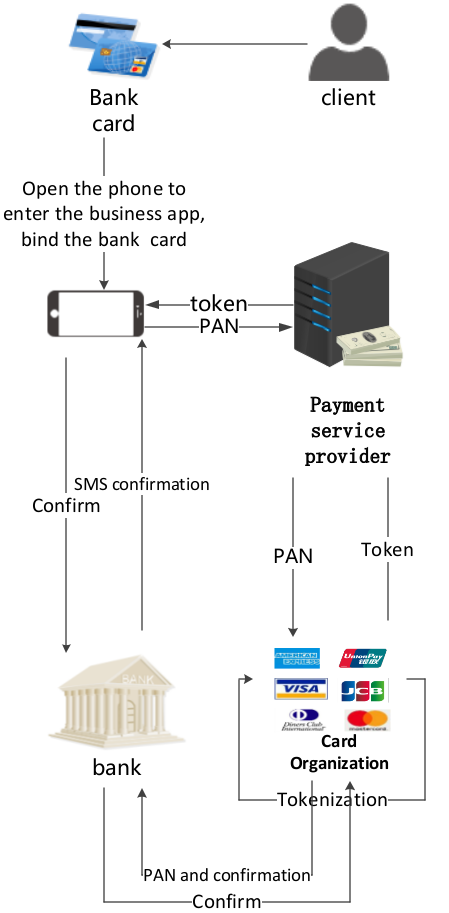
\includegraphics[scale=0.5]{tsp1.png}}
\caption{Token application process.}
\label{fig}
\end{figure}

  The international chip card standardization organization EMVCo has defined smart card payment and also defined a token as a substitute in the actual card application. Merchants can handle cards and tokens in the same way, which means that there is no need to change the already installed and installed PoS (Point of Sale) terminals. This clever processing is done through a Token Service Provider (TSP) that has the actual card information. When issuing token Tokens, you can flexibly make some restrictions, such as the use of only certain businesses, online use only, offline use, and you can limit the value, time and location of tokens, such as The security level of the device determines its effective time. When necessary, tokens can be destroyed and re-issued. The Tokens solution ensures compatibility with existing infrastructure and saves money. Working with HCE, the token can solve the problem of availability. When the mobile network is unstable, the token is stored locally on the mobile phone and can be paid offline. The EMVCo Payment Token Specification Technical Framework v1.0 provides examples of secure storage of tokens on a device. For example, it can be stored in a trusted execution environment TEE. In addition, tokens can be used through any channel, such as NFC, Internet transactions, and Bluetooth Beacons, so the technology is not limited to PoS terminals.
  
As described in [10], a tokenization system has the following components:

\textbf{1.A method for token generation}
A process to create a token corresponding to a primary account number (PAN). Some of the mentioned options are encryption functions, cryptographic hash functions and random number generators.

\textbf{2.A token mapping procedure}
It refers to the method used to associate a token with a PAN. Given a token, this method will allow the system to recover PAN.

\textbf{3.Card-Vault}
It is a repository that typically stores pairs of PANs and tokens and other information needed for token mapping. Since it may contain PAN, it must be specially protected according to PCI DSS requirements.

\textbf{4.Cryptographic Key Management}
This module is a set of mechanisms for creating, using, managing, storing, and protecting keys used to protect PAN data and data involved in token generation.
\\

It is two basic requirements for tokens and tokenization systems.

\textbf{Format Preserving}
The token should have the same format as the PAN so that the stored PAN can be easily replaced by the token in the merchant's environment. At the same time, it has to be detected by the luhn algorithm, In addition, it is important to distinguish the token from the PAN to token and the PAN issuer easily. Finally, it also needs convenient to distinguish the card issuer of the PAN corresponding to the token.

\textbf{Uniqueness}
The token generation method should be deterministic. The tokens for a specific PAN should be unique,In a specific payment environment two different PANs should be represented by different tokens.

Article [10] discusses the security of tokenization systems.the author consider three different attack scenarios: 

\textbf{1. IND-TKR }: Tokens are only public. This represents the most realistic scenario where an adversary has
access to the tokens only, and the card-vault data remains in-accessible.

IND-TKR refers to the basic security requirement for tokens. It adheres to the informal security notion for tokens as stated in the PCI DSS guideline for tokenization. It models the fact that tokens and PANs are un-linkable in a computational sense, if the key and card-vault are kept secret. Thus, if a merchant adopts a tokenization scheme provided by a third party, which is secure in the IND-TKR sense then this will probably relieve it from PCI compliance. As in this case the merchant does not own the card-vault or the keys, and the burden of security involved with the keys and the card-vault lies with the provider who offers the tokenization service.

\textbf{2. IND-TKR-CV }: The tokens and the contents of the card-vault are public. This represents an extreme scenario where the adversary gets access to the card-vault data also.

The IND-TKR-CV is a stronger notion. If a tokenization system achieves this security, then it implies that tokens and PANs are un-linkable even with the knowledge of the card-vault. This in turn implies that the contents of the card-vault are not useful (in a computational sense) to derive a relation between PANs and tokens. Thus, it provides security both to the tokenization service provider and the merchant who use this service.

3. IND-TKR-KEY : This represents another extreme scenario where the tokens and the keys are public.

IND-TKR-KEY is a stronger form of the IND-TKR notion. Some public documents like [17] it has been stressed that encryption is not a good option for tokenization, as in theory there exists the possibility that a token can be inverted to obtain the PAN. If tokens are generated using a “secure” encryption scheme, then it is infeasible for any “reasonably efficient” adversary to invert the token without the knowledge of the key. But, this computational guarantee does not seem to be enough for users. The IND-
TKR-KEY definition aims to model this paranoid situation, where linking the PANs with tokens becomes infeasible even with the knowledge of the key. Note in IND-TKR-KEY we still assume that the card-vault is inaccessible to an adversary.
\\

All the definitions follow the style of a chosen plaintext attack. The definitions may be made stronger by giving the adversary additional power of obtaining PANs corresponding to tokens of its choice. But in this application, we think such stronger notions are not applicable.

the [10] also give the security proof of Tokenization Using FPE and Tokenization Without Using FPE.For details, please check the the article

Tokens and tokenization solutions can be implemented in numerous ways, and the security or process controls provided by one solution may not be suitable or applicable to another. Additionally, the assignment of roles and responsibilities may vary according to the particular solution or deployment method, and all entities involved should be aware of their obligations for maintaining security controls and protecting cardholder data.[10]

The level of PCI DSS scope reduction offered by a tokenization solution will also need to be carefully evaluated for each implementation. For example, locations and flows of cardholder data, adequacy of segmentation, and controls around de-tokenization and mapping processes should be reviewed and verified to ensure proper scoping of the CDE and appropriate application of PCI DSS security requirements.[10]
\subsubsection{Centralized tokenization technologies}
Centralized tokenization is conventional, database-centric solutions,which requst the token corresponding to the provided PAN from a common central database, as described above. If no token corresponding token exists in the common central database at the time of the request, a new token is generated and an entry will be added to the common central database.


\begin{figure}[htbp]
\centerline{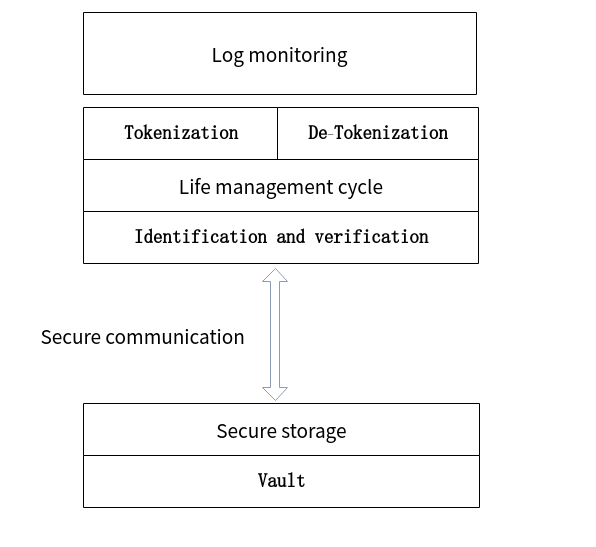
\includegraphics[scale=0.4]{tsp.png}}
\caption{tokenization service provider of centralized tokenization scheme}
\label{fig}
\end{figure}
 
Card organizations are highly recommended centralized tokenization technologies. 
Centralized tokenization involves building a large-scale database (“token vault”), storing each PAN together with a generated token. Figure 3 shows the China UnionPay payment tokenization system framework


\subsection{Distributed tokenization technologies}
Although traditional centralized tokenization has been widely used, it has also been exposed some critical problems[19]:

$ \bullet $ Complexity and cost: Managing large, replicated token databases is difficult and costly, and these databases themselves increase PCI audit scope. 

$ \bullet $ Integrity: In accurate analytics and other application correlation due to credit card numbers sometimes being replaced by more than one token (a side effect of having a distributed token database).

$ \bullet $ Security and risk: Approaches without independent and reviewable security proofs increase breach risk and do not meet QSA(Quality 
Security Assessor) evidence requirements, and thus cannot achieve PCI compliance. In the event of a breach that leaks cardholder details, merchants using such approaches have no grounds to avoid significant penalties.

$ \bullet $ Performance and scale: Tokenization performance is slow and very difficult to scale.

 PCI use case completeness: Tokenization is not suited to offline environments, such as web browsers or card swipe terminals. Supplementary solutions are required for PCI DSS audit scope reduction in such applications.

In response to these problems, many companies have proposed distributed tokenization schemes one after another. The main feature is that the generation of tokenization is not concentrated in one server, but can be distributed in various places. Each place can generate the same unique token.


\begin{figure}[htbp]
\centerline{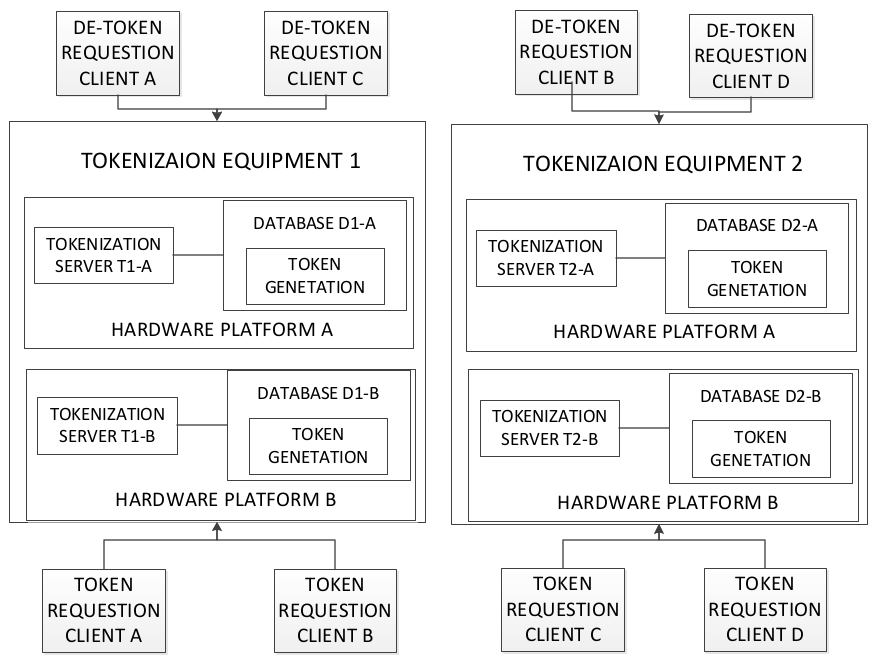
\includegraphics[width=9cm,height=9cm]{dis_token.png}}
\caption{Distributed Tokenization Scheme of MICRO FOCUS}
\label{fig}
\end{figure}

Figure 4 shows the distributed tokenization scheme of MICRO FOCUS[20]. Tokenization equipment can be used for tokenziation and de-tokenization. And it can have multiple and distributed in different geographical locations. User A may exchange tokens for PAN in tokenization equipment A, and may request de-tokenization operations in tokenization equipment B, and vice versa. In this way, there can be no data center dedicated to manage tokenization and de-tokenization, but can operate on any tokenization equipment.

The token generation process of mainstream distributed tokenization scheme consists of the following features:

$ \bullet $ Pre-positioning the same lookup tables to each tokenization equipment. Lookup table of MICRO FOCUS schem[20] as shown in table 1.

$ \bullet $ Using lookup tables to design mapping schemes, often using iterative mapping, rotation, etc.

$ \bullet $ Don't store the mapping relationship between PAN and token. 

The distributed solution relieves some problems of the centralized system to some extent. In particular, the elimination of centralized data centers can greatly reduce costs. However, new issues have also been traced. Once the lookup table leaks, it will have a major impact on the security of the entire solution. Moreover, the lookup table is the same in all local devices. On the other hand, it is not very convenient to withdraw tokens.



\begin{center}
\textbf{Table 1}~~Lookup Table.\\
 \setlength{\tabcolsep}{1mm}{\begin{tabular}{|c|c|} %l(left)居左显示 r(right)居右显示 c居中显示
\hline 
TOKEN&SENSITIVE NUMBER\\
\hline  
4876 9865&2348 9286\\
\hline
7374 2625&2827 6438\\
\hline
...&...\\
\hline
...&...\\
\hline
...&...\\
\hline
&\\
\hline
&\\
\hline

\end{tabular}}
\end{center}






\subsection{The process of binding bank card.}
Tokenization is a key link for binding a bank card to a mobile phone, but the security of the entire process also requires the application of multiple technologies. Since distributed tokenization are not widely used, the following are discussed in centralized tokens.

In the entire process, apart from the customer himself, two departments have played a major role:

\subsubsection{TSP(Token Service Provider)} The TSP is mainly responsible for the Token management related work in the Tokenization system, and maintains a series of components related to Token operations. The TSP provides the services provided by these components in the form of APIs for other roles to call, mainly including the following aspects: .

\textbf{1)} Tokenization component;
 
\textbf{2)} De-Tokenization component;
 
\textbf{3)} ID\&V components:During the Token generation process, the user's account number needs to be verified to assign different guarantee levels to the Token. Different guarantee levels limit the range that the Token can use. This verification is performed by the ID\&V component. ID\&V actually accepts sensitive information from a group of users and outputs the user's Token security level after a certain algorithm;
 
\textbf{4)} Token Lifecycle Management Components;
 
\textbf{5)} Token and Card Data Vault:The Token vault is the core of data storage in the TSP. In addition to the mapping between the user Token and the PAN, it also stores the sensitive information that the user uses for the ID\&V process. There is no such thing in the distributed tokenization scheme.

TSP is mainly undertaken by card organizations, banks, or some large financial companies.




\subsubsection{TR(Token Requestor)}
TR is mainly responsible for two aspects of work in this payment system.

On the one hand, TR needs to provide a set of APIs for developers of electronic wallets. The API includes two parts:

1) The first part of the API provides cardholder lifecycle management, such as user registration, user login, and user revocation.

2) The second part is the interface related to the Token service, including the application, update, unbundling, and loss reporting of the Token.

On the other hand, when the TR receives the Token application request of the user, it needs to call the corresponding API of the TSP to route the request to the corresponding TSP, and then the TSP returns the value of the Token and some other related data and finally forwards it to the user.

In today's market, TR is mainly played by payment service providers. TR first needs to register with the TSP. The registration process and the data involved may differ according to different TSPs. After the registration is completed, TSP assigns a unique ID (Token Requestor ID) to the TR for the TSP to identify the legitimacy of the TR. Each TR ID corresponds to a TSP, so a TR can have multiple TR IDs. After the TR can apply for the Token, the specific way to call the API interface provided by the TSP.

Figure 1 shows the mainstream process of binding bank cards to mobile phones today:

1,Open the payment software app and start binding the bank card and enter PAN;

2,The phone sends the PAN over the encrypted channel to the server of the payment service provider, 

3,The payment provider hands over the bank card account (PAN) which the user needs to bind to the corresponding bank server. If the corresponding virtual bank card for this PAN does not exist for this merchant in the public central database,a new virtual is generated and an entry is added to the public central database.At the same time return virtual bank card to the merchant. The merchant binds the token with the user's account as a virtual bank card corresponding to the PAN.

4,The card company confirms with the card issuing bank of the PAN, and then the card issuing bank sends a random code to the user's mobile phone through the short message, allowing the user to enter the random code on the mobile phone for confirmation.

5,After the user confirms, the issuing bank will reply with confirmation information to the card organization. The card organization uses the TSP to generate a token reply to the payment service provider, which then stores the token on the server and responds to the user's mobile phone.

6,Finally bind tokens to mobile terminals instead of PAN for mobile payment transactions


\begin{figure}[htbp]
\centerline{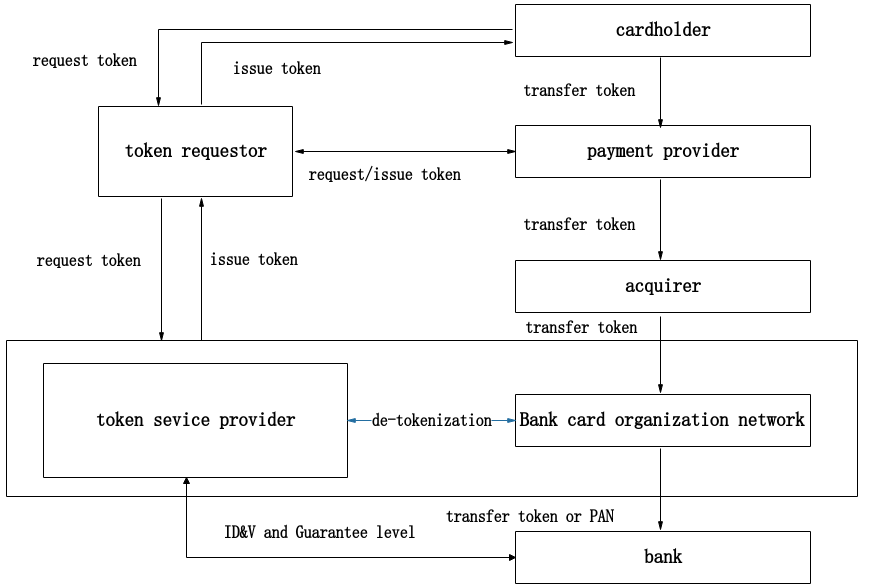
\includegraphics[width=9.5cm,height=7cm]{zhifubiaojikuangjia.png}}
\caption{China UnionPay payment tokenization system framework}
\label{fig}
\end{figure}

Figure 3 shows the payment system framework of China UnionPay. Its entire bank card binding process is basically the same as described above. However, during this process, if the payment service provider maliciously saves the PAN, it is difficult to deal with it.



However, in order to prevent the payment provider to saving or leaking the user's real bank card information, Alipay has proposed a new virtual bank card binding scheme. As shown in Figure 5:

1, the merchant system pre-save the payment system server authorization certificate. And authorize the signature of the authorization certificate called its default instructions.

2. The merchant system receives a binding request sent by a terminal, where the binding request corresponds to a user account that the user logs in on the merchant system; and returns a preset instruction to the terminal;

3, the terminal to the payment system through the secure channel to send the default instructions and the real bank card number.

4, the payment system generates a virtual bank card number corresponding to the real bank card number. (For each real bank card number generated by the virtual card number is different)

5, the virtual bank card number returned to the terminal.

6, the terminal sends the virtual bank card number to the payment provider.

7, the payment provider bind the virtual bank card to the user accounts.

In this scheme, the payment provider can not get the user's real bank card account information.

\begin{figure}[htbp]
\centerline{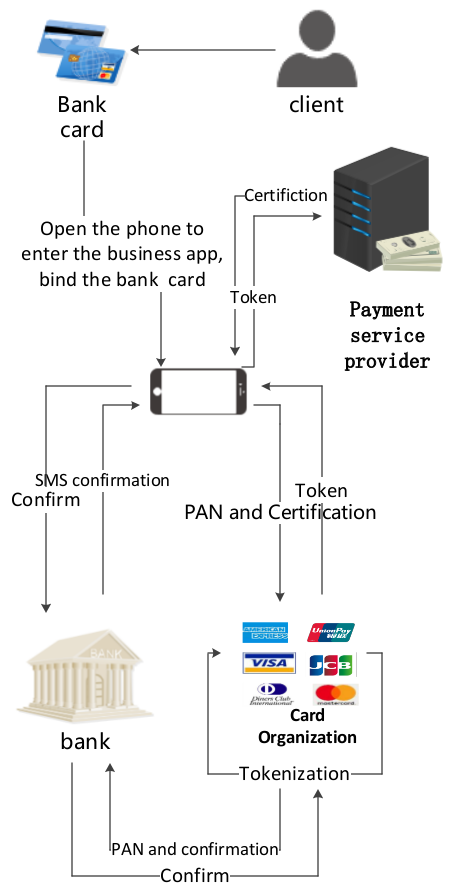
\includegraphics[scale=0.5]{tsp2.png}}
\caption{Token binding process.}
\label{fig}
\end{figure}

The PAN leak is really avoided in Alibaba's solution.

The tokenization technology and bank card binding scheme are the bottom layer of mobile payment technology. The former centralized solution needs to solve the problem of large-scale data storage and a single token generation location, and the distributed solution needs to solve the problem of the leakage of the lookup table. The latter needs to solve the problem of PAN being hijacked by a third party during the binding process.



\section{Mobile Terminal Security}
After the mobile phone binds the token, it begins to act as a mobile payment terminal. The mobile terminal need often authenticates the payment and also stores a lot of sensitive information, such as the PIN code of the payment APP,fingerprint and the token. Once the mobile payment terminal is invaded by an adversary, the customer will suffer heavy losses. Therefore, the security of mobile terminals is also increasingly concerned by major mobile phone manufacturers and payment service providers.

TEE and eSE are the two key technologies for the security of mobile terminals in mobile payment today.


\subsection{TrustZone}
In 2006, the open mobile terminal platform organization OMTP (Open Mobile Terminal Platform) took the lead in presenting a dual system solution: that is, in addition to a multimedia operating system, providing an isolated security operating system under the same intelligent terminal. Isolated security operating systems on isolated hardware are used to specifically process sensitive information to ensure information security. This program is the predecessor of TEE.

Based on the OMTP solution, ARM (the world's largest solution provider of embedded processors whose architectures account for approximately 95\% of the mobile phone market) proposed a hardware virtualization technology TrustZone and related hardware in 2006. Implement the plan. TrustZone is a product that supports TEE technology. TrustZone is the basic function of all Cortex-A processors. 

TrustZone conceptually divides SoC hardware and software resources into Secure World and Normal World. All operations that require confidentiality are performed in the secure world (such as fingerprint identification, password processing, data encryption and decryption, and security certification, etc.) The rest of the operations are performed in a non-secure world (such as user operating systems, various applications, etc.), the security world and the non-secure world are converted by a mode named Monitor Mode.

On the processor architecture, TrustZone virtualizes each physical core into two cores, a non-secure core (NS Core), which runs a non-secure world, and another secure core (Secure Core), which run the safe world code.

The two virtual cores operate in a time-sliced manner, occupy physical cores in real time as needed, and switch between the secure world and the non-secure world through Monitor Mode, similar to a multi-application environment under the same CPU, but different from multiple applications. In the program environment, the operating system implements inter-process switching, while the Monitor Mode under Trustzone implements switching between two operating systems on the same CPU.

For more details, please refer to the TrustZone white paper [15].

\subsection{TEE}

ARM later provided its TrustZone API to GlobalPlatform, which has evolved into a TEE client API. It is introduced through the ARM architecture security extension, and ARM has become one of the leaders of TEE technology.


GlobalPlatform (the world's leading organization for smart card multi-application management specification, abbreviated as GP) is an international standard organization led by Visa, MasterCard, and other international bank card organizations. Since 2011, it has drafted and developed related TEE specification standards, and has joined several companies. (ARM, etc.) jointly develop a trusted operating system based on the GP TEE standard. Therefore, most of today's Trust OS based on TEE technology has followed the standard specification of GP.



The Trusted Execution Environment (TEE) is a concept proposed by the Global Platform (GP). For the open environment of mobile devices, security issues are also getting more and more attention, not only terminal users, but also service providers, mobile operators, and chip vendors. TEE is an operating environment coexisting with Rich OS  on the device and provides security services to Rich OS. It has its own execution space, which is higher than Rich OS's security level, but lower than the security element (SE, usually a smart card). However, TEE can meet the security needs of most applications. From a cost perspective, TEE provides a balance between security and cost.
 
\begin{figure}[htbp]
\centerline{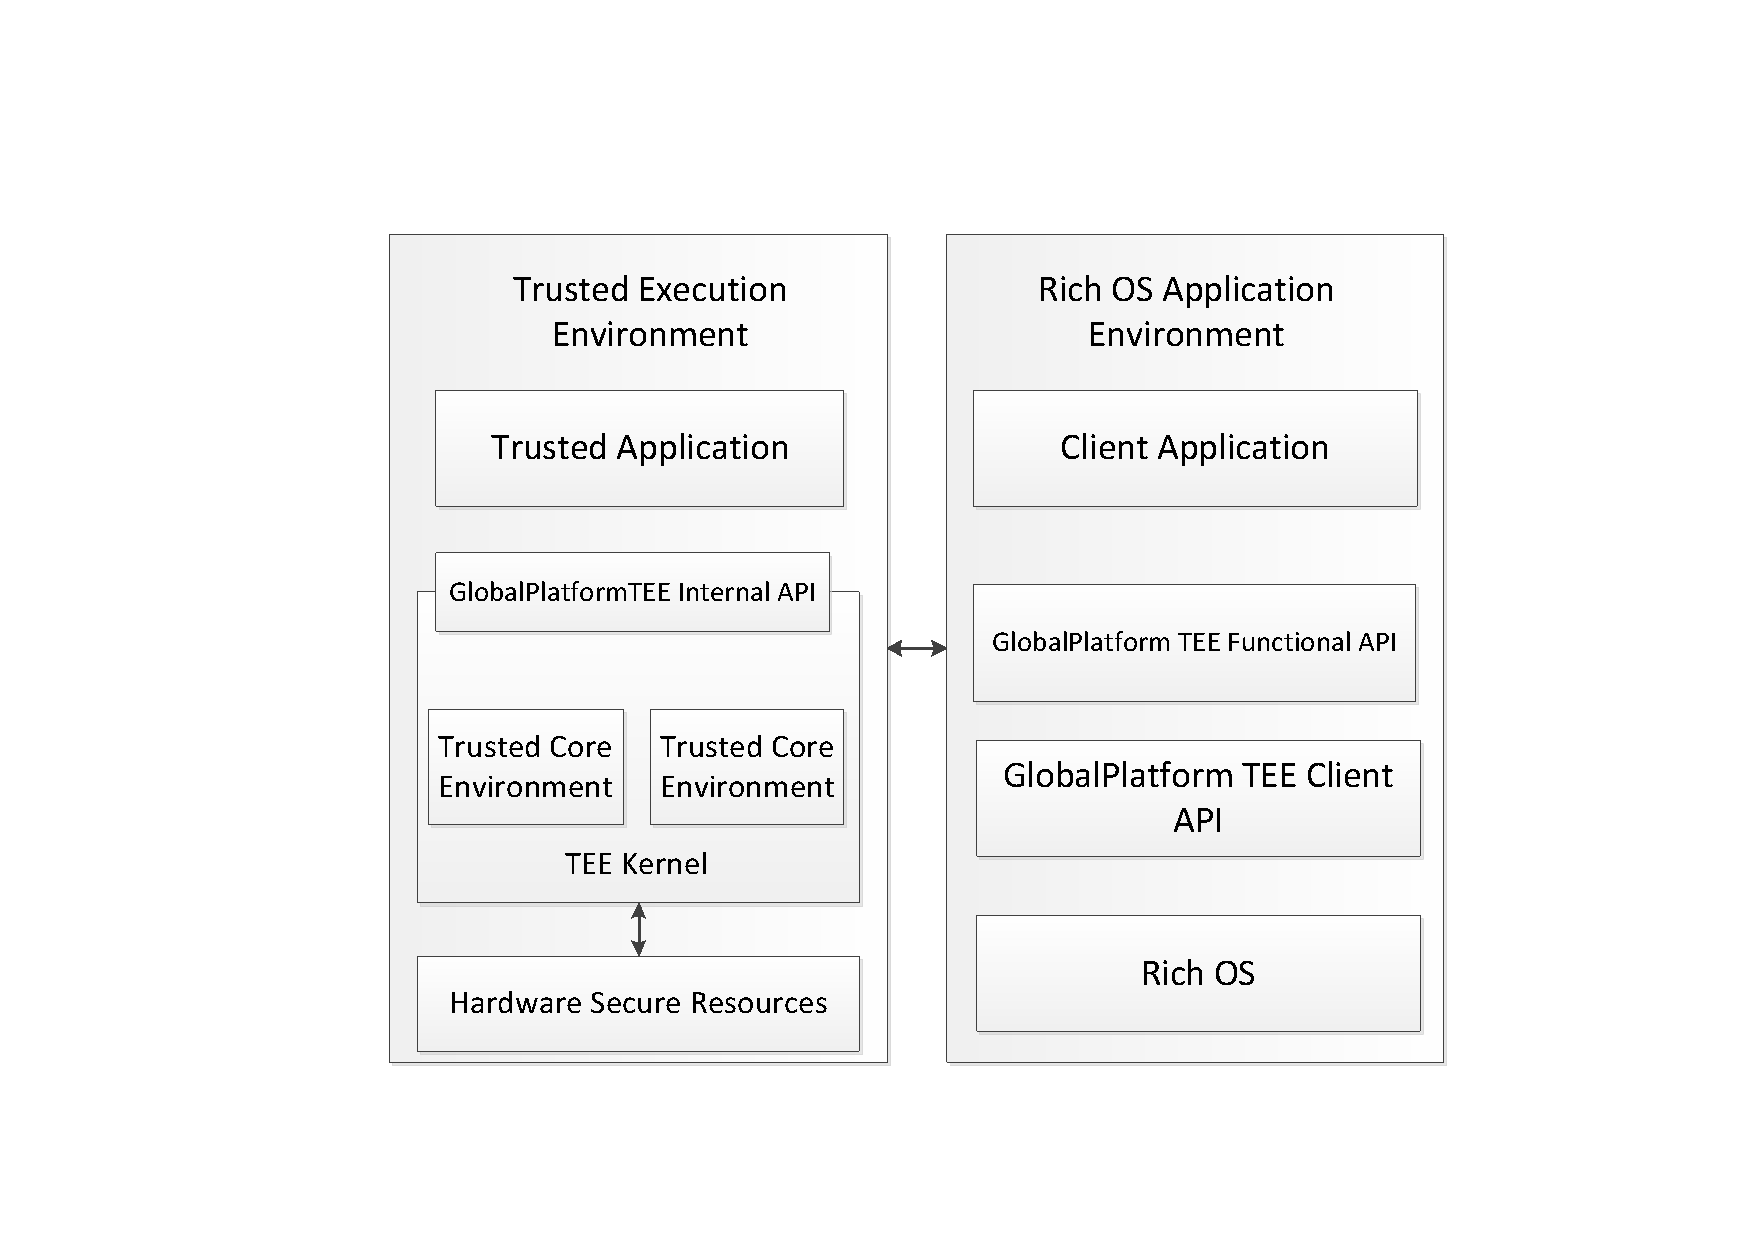
\includegraphics[scale=0.5]{TEE.pdf}}
\caption{TEE and Rich Os}
\label{fig}
\end{figure}

Among them, the software and hardware resources that TEE can access are separated from Rich OS. TEE provides a secure execution environment for authorized security software (\textbf{trusted applications, TA}) while also protecting the confidentiality, integrity, and access rights of TA's resources and data. To ensure the trusted root of the TEE itself, the TEE is authenticated and isolated from the Rich OS during the secure boot process. In TEE, each TA is independent of each other and cannot be accessed without authorization.

GP has made great efforts in the standardization of TEE. The basic specifications include TEE internal API, TEE client API, and of course, there are a series of additional functional API specifications, as well as application management, debugging functions, security protection profile, etc. In development.

The TEE internal API mainly includes APIs such as key management, cryptographic algorithms, secure storage, secure clock resources and services, and an extended trusted UI. Trusted UI means that when key information is displayed and user key data (such as password) is input, hardware resources such as screen display and keyboard are completely controlled and accessed by TEE, and software in Rich OS cannot be accessed. The internal API is the programming interface that TEE provides to TA;

The TEE external API is the underlying communication interface for the client application  unning in the Rich OS to access TA services and data.


\subsection{SE}
Secure Element (SE) is a platform that can install, personalize and manage applications. It is a combination of hardware, software, interfaces, and protocols that can securely store and use credentials for payment, authentication, and other services. Conceptually, SE can be divided into two areas from the paper [17] :

$\bullet$ Embedded SEs;

$\bullet$ Removable SEs;


\subsubsection{Embedded SE}
The embedded SE is a chip that is integrated into a mobile phone and cannot be removed. According to research [18], the SE provides the same level of security as smart cards support. The chip is embedded in the handset during the manufacturing process and must be personalized after the device is delivered to the end user [18]

The eSE is the most secure device in mobile phones and often stores fingerprint data with the highest security level, authentication keys, and bank card related information. High-end mobile phones often equipped with fingerprint recognition will be equipped with eSE. For example, iphone 7/8, Samsung s9, Huawei mate 10, etc.

\subsubsection{Removable SEs} The rSE is a chip that can be removed and replaced in mobile phones. Usually embedded in some replaceable phone hardware
, such as SD card, SIM card

\emph {SMC:} The Secure Memory Card (SMC) provides the same advanced security as a smart card and meets most of the smart card's major standards and interfaces (eg, GlobalPlatform, ISO/IEC 7816, JavaCard, etc.). As described in [18], SMC can host a large number of applications with mobility and large memory. 

This year, SMC has slowly withdrawn from the market because major mobile phone manufacturers are no longer supporting SD cards.

\emph {UICC:}  Cards used in existing mobile phones such as SIM, USIM, UIM, etc. are collectively referred to as UICC(Universal Integrated Circuit Card.)

UICC is a general multi-application platform for implementing smart card applications of SIM or USIM. UICC provides an ideal environment for personal, secure, portable and easily remotely managed NFC applications via OTA technology. It can host non-telecom applications from various service providers such as loyalty, ticketing, healthcare, access control and ID applications. GlobalPlatform provides the most promising standard for UICC life cycle management (or card content management)[17].


\subsection{comparision}
The TEE is running in the device and provides a framework for security between ordinary RichOS and SE (smart card). Many current security architectures are based on Rich OS + SE. In fact, this cannot provide a "just good" fit in terms of convenience and cost. Because some small payments, DRM, corporate VPN, etc., the required security protection is not high, does not need a separate SE to protect, but it can not be directly in Rich OS, because of the latter's openness Make it easy to be attacked. So for such applications, TEE provides the appropriate protection strength and balances cost and ease of development.

For attack resistance, SE is the highest and Rich OS is low. For access control, it is similar to anti-attack, but Rich OS can do more; for the user interface, SE is powerless, and Rich OS is the most abundant; development is easy. On the other hand, the Rich OS is the easiest. Of course, if the TEE standard is done well, it can be done quite "easy". On the processing speed, TEE and Rich OS are equivalent. Because the same physical processor used by both, SE is certainly slow; Finally, the SE is physically removable.

After joining TEE, the extra cost increase is very low, and it can reach a medium protection level; if you want to achieve high-level protection, you will need additional costs. The analysis of this figure does not mean that the appearance of TEE makes the device not need SE, but as a medium security level, to meet the corresponding security objectives.
\\
\begin{center}
\textbf{Table 1}~~Comparison.\\
 \setlength{\tabcolsep}{1mm}{\begin{tabular}{|p{2cm}|p{2cm}|p{2cm}|p{2cm}|} %l(left)居左显示 r(right)居右显示 c居中显示
\hline 
&REE&TEE&SE\\
\hline  
 &Only software&Software and HW&Software and Tamper 
resistant HW\\
\hline
Cost&No extra cost&Low extra cost&High extra cost\\
\hline
Attack Resistance&Weak&General&Strong\\
\hline
Access Control&Weak&General&Strong\\
\hline
User Interface&Abundant&Can do a little&Powerless\\
\hline
Ease of Development&Easy&Easy with right Standard&Hard\\
\hline
Processing Speed&Fast&Fast&Slow\\
\hline
 
\end{tabular}}
\end{center}


With the support of major chip manufacturers, mobile phones using ARM architecture chips now include Trustzone technology. The gap between the real high-end phones and low-end phones is on eSE. In addition to PIN payment authentication, fingerprints are supported by high-end handsets of major mobile phone manufacturers. iphone X now supports face recognition. It is very necessary to store these sensitive information in eSE.

\section{Payment communication technologies}
After obtaining a secure payment mobile terminal, how to ensure payment communication security has become a hot topic in this field.

Payment communication technology is intuitively experienced by customers. In the customer's eyes is how to pay the money to the recipient. For example, Alipay, WeChat, etc. are called QR code payment. While Apple, Samsung, etc. are often called NFC payments. In fact, the former only uses a two-dimensional code to transfer one-time payment passwords. What really pays for the payment is the one-time payment password. Whatever the method, as long as you can transfer the one-time payment password, you can conduct a payments, such as audio. The latter's NFC is actually an interactive near-field communication.

\subsection{QR code}
QR code was invented in 1994 by Denso Wave, a Toyota subsidiary of Japan. The QR code not only has large information capacity, high reliability, and low cost, but also can represent various character information such as Chinese characters and images, and has strong security against fraud and is very convenient to use. Therefore, it quickly became popular in Japan and South Korea. Since then, European and American countries have begun to use it in large quantities. 

QR code payment is very popular in China, people can almost go out without wallets and bank cards. You only need to show the QR code on your mobile phone to be able to pay in most places even without network. However, why is it possible to authorize payment with the QR code?

However, the QR code itself cannot make payment authorization, since the actual payment authorization is the one-time payment password which encoded in the QR code. The one-time payment password is a series of digits(which we calld \textbf{payment password}). You can authorize payment with this numbers. So the role of the QR code in mobile payment is to transmit this series of numbers. The specific technology of one-time payment password will be told in section 6.

In this subsection, the QR code technology will be introduce.

The QR code is one of the two-dimensional code, which is similar to the magnetic stripe. The magnetic stripe transforms the information into a track through a certain law, and the two-dimensional code transforms the information into a graph. Reading the magnetic stripe reads the track through the reader and then converts back to the original information, while the two-dimensional code reads the graphics through the camera and then converts back to the original information.

\textbf{Stacked two dimensional bar code:} It consists of multiple rows of bar codes stacked together. Its shape is similar to that of one-dimensional codes. The encoding principle is similar to the encoding principle of the same dimension codes. It has the same or similar characteristics as the one-dimensional bar code in terms of coding design, reading mode, and verification principle, and can even be read and scanned with the same device, except that the reading and decoding algorithms are different from the one-dimensional bar code. Larger capacity but usually does not have error correction.
Representatives are cod 49(shows at Fig 7) and PDF 417(shows at Fig 8):


\begin{figure}[htbp]
\centerline{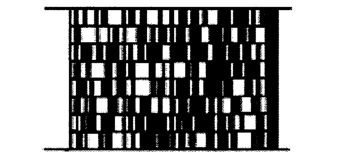
\includegraphics[scale=1]{code49.png}}
\caption{code 49}
\label{fig}
\end{figure}


\begin{figure}[htbp]
\centerline{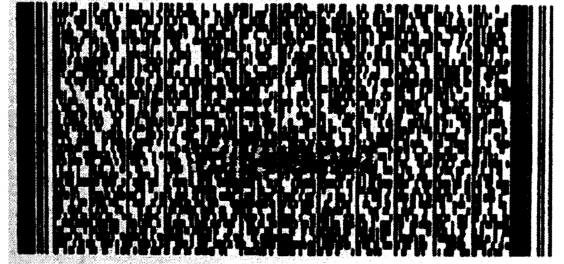
\includegraphics[scale=0.5]{PDF417.png}}
\caption{PDF 417}
\label{fig}
\end{figure}

\textbf{Matrix type two-dimensional bar code:}
A matrix consisting of dark squares and light squares, usually square, where the dark and light blocks represent 1 and 0 in binary, respectively. Matrix-based two-dimensional code is a graphical symbol automatic identification and processing code system, which usually has error correction function. Typical examples are DM codes, QR codes, and Hanson codes.

The QR code has a total of 4 error correction levels, represented by L, M, Q, and H, respectively, and the recoverable code word ratios are 7\%, 15\%, 25\%, and 30\% in order. The higher the error correction level used is, the more error correction code words are used, and the fewer code words are used for encoding information. (In which the related technology mainly uses error correction code)

\begin{figure}[htbp]
\centerline{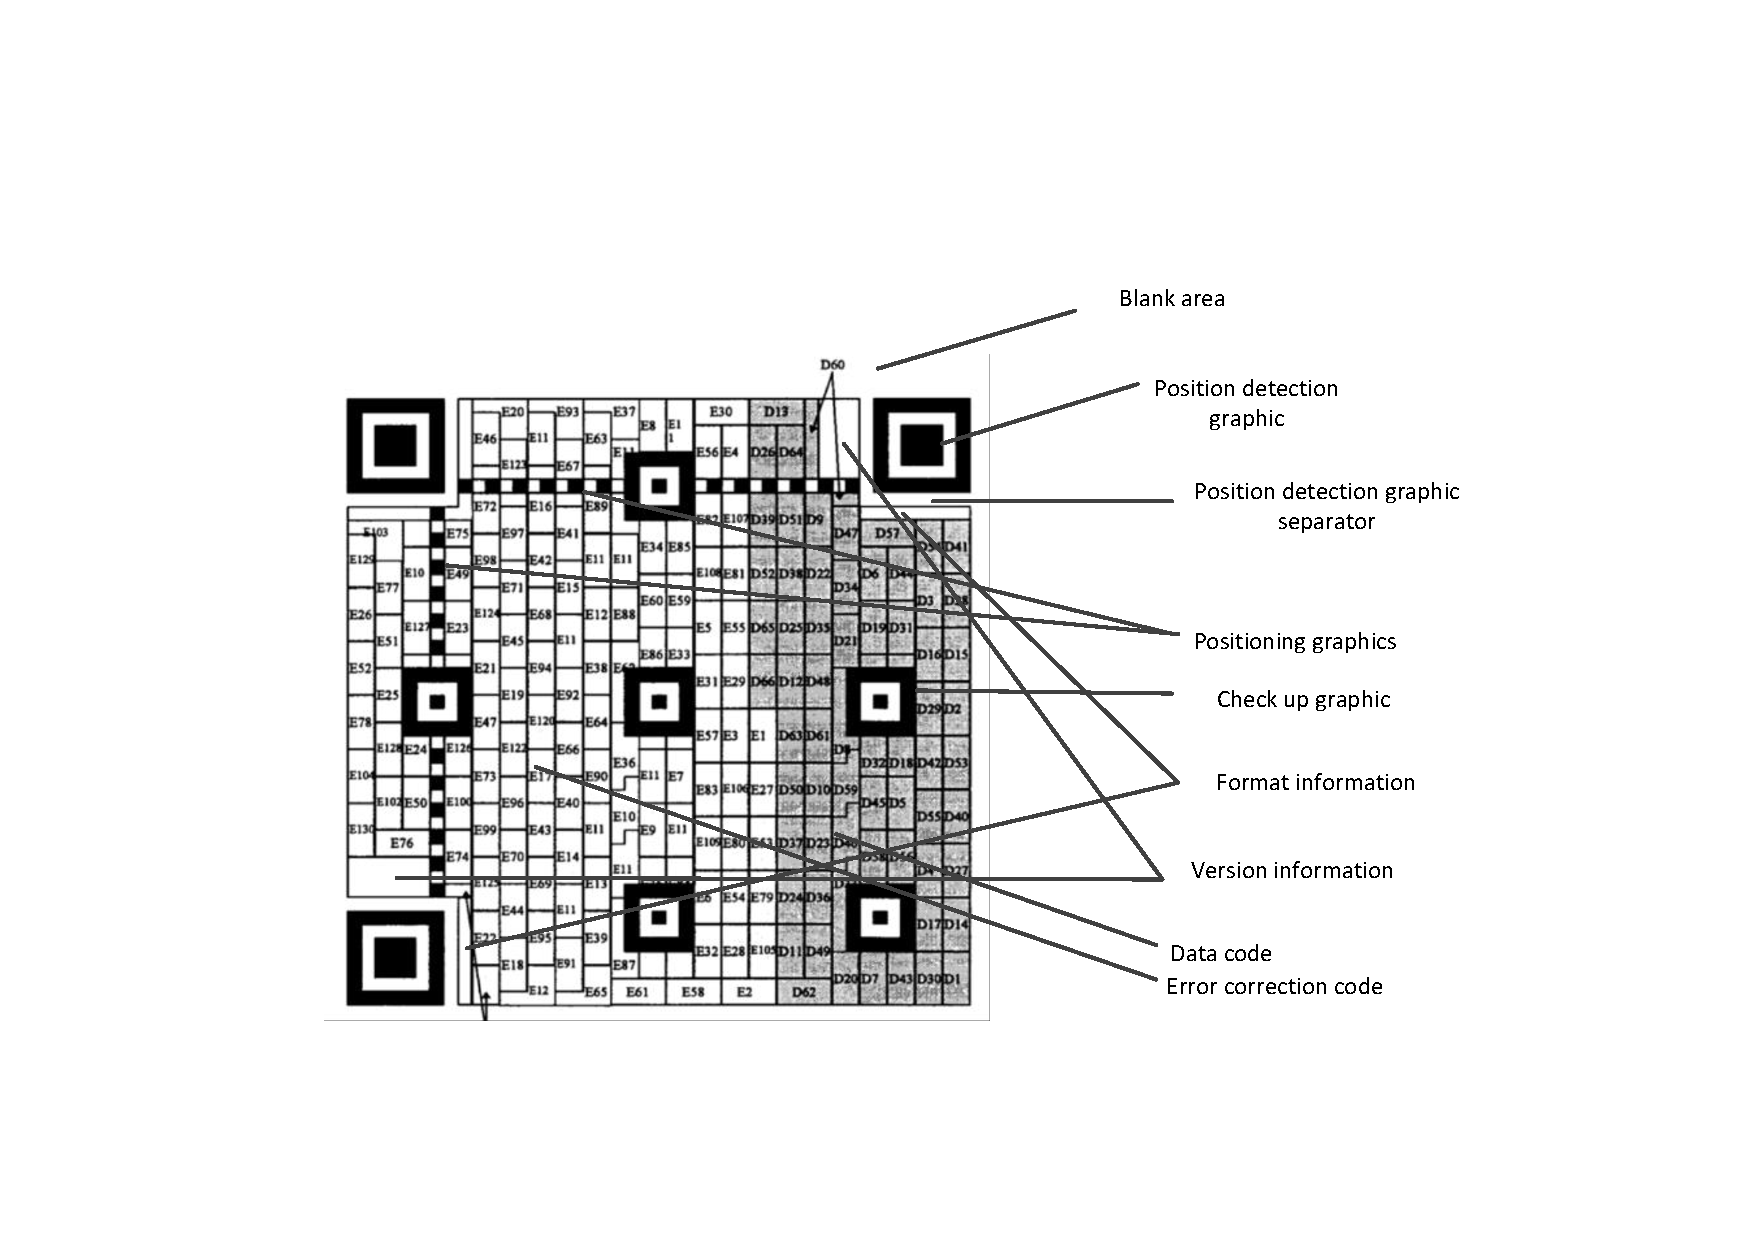
\includegraphics[scale=0.46]{QRcode.pdf}}
\caption{The structure of the QR code}
\label{fig}
\end{figure}

The Fig 7 shows the structure of the QR code:

\textbf{Check up graphic:}The Check up graphic looks similar to the position detection pattern, but the middle square has only one unit. It is mainly used for the correction of the QR code, especially the correction of the graphic distortion caused by the different camera angles or the uneven surface of the printed object. Depending on the version, the number of correction patterns is not the same. There is no correction pattern for version 1 and version 40 contains 46. Wechat's payment code belongs to version 1 so there is no correction graphics, and Alipay's payment code belongs to version 2, there is one.

\textbf{positioning graphic:}The positioning graphic is two alternating dark and light bands, and the table is defined on the two-dimensional code like a ruler.

\textbf{Format and Version information:}The format information and version information record the format and version of this QR code and have their own separate calculation rules.

\textbf{Data and Error Correction code:}After the error correction coding of the data is completed, the final code word sequence is constructed in a certain order for the data code word and the error correction code word. The low code word of each data block is in front of the sequence, and the data code word is arranged in front of the error correction code. According to the first codeword of data block 1, the first codeword of data block 2, ..., the last codeword of data block n; the first codeword of error correction code 1, error correction The second codeword of code 2, ..., the last codeword of error correction code n


\subsection{NFC}
NFC is a technology that mobile phone manufacturers strongly recommend in the field of payment communications. Many new mobile phones released by Apple, Samsung, Google, Xiaomi, Huawei, etc. all support NFC. 

Near field communication (NFC) is a wireless technology operating in the short range of four to ten centimeters for communication. It is based on radio frequency identification (RFID) technology. For a communication, an NFC device generates a radio frequency in 13.56 MHz spectrum. A receiver could receive the data through the principle of magnetic inductive coupling if it lies in a close proximity. Transmitter and receiver are small chipsets which are able to be embedded in devices such as mobile phones, POS (Point Of Sale) terminals, cards posters and many other items. 

The NFC forum was formed in 2004 aimed at standardizing NFC technology. It defines NFC as: NFC is a short-range wireless connectivity technology (also known as ISO 18092) that provides intuitive, simple, and safe communication between electronic devices. Operating at the frequency of 13.56 MHz and limited short range communicating distance, NFC supports data rate of 106 Kbps, 212 Kbps and 424 Kbps. Therefore, NFC is suitable for transmission of short information or messages within small time interval. 

In recent days, NFC technology is being widely popular among mobile phone vendors and related fields. This is because NFC is compatible with already existing popular technologies such as RFID, smartcards and contactless cards. It means that stores and systems equipped with the existing technologies should not replace their infrastructure in order to support NFC. 

The incorporation of NFC into mobile devices has augmented capability of mobile phones and it is predicted to have potential to do more. This phenomenon has brought forward various works in terms of NFC transactions. At the same time, however, there are serious concerns in different terms such as privacy, user satisfaction, speed, usability, etc. Moreover, it is replacing various popular devices such as RFID tags. Hence, it is important to evaluate the performance of NFC technology and where it stands. 

\begin{figure}[htbp]
\centerline{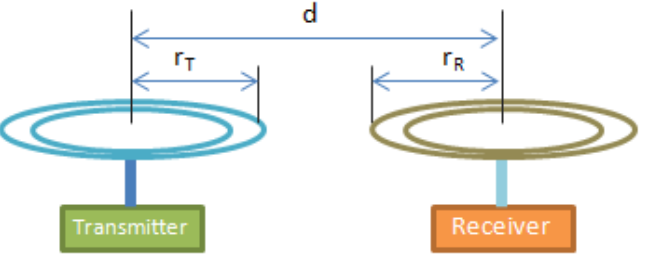
\includegraphics[scale=0.35]{InductivelycoupledNFCantennas.png}}
\caption{A complete sound packet.}
\label{fig}
\end{figure}

NFC devices communicate through the magnetically induced signals. Therefore, during transmission, energy is coupled between transceivers instead of electromagnetic radiation as in traditional wireless communication. The magnetic induction is discussed in detail in []. The magnetic induction theory and its application to NFC are also discussed. Figure 4 shows inductively coupled NFC antennas separated by short distance usually in the units of centimeters. Within close proximity, information can be exchanged between these transceivers by magnetic induction. Equivalent circuit diagram of these antennas is shown in Figure 5.Mathematical derivation of power at the receiver for given circuit is derived in [2], where power at the receiver can be expressed as

\begin{figure}[htbp]
\centerline{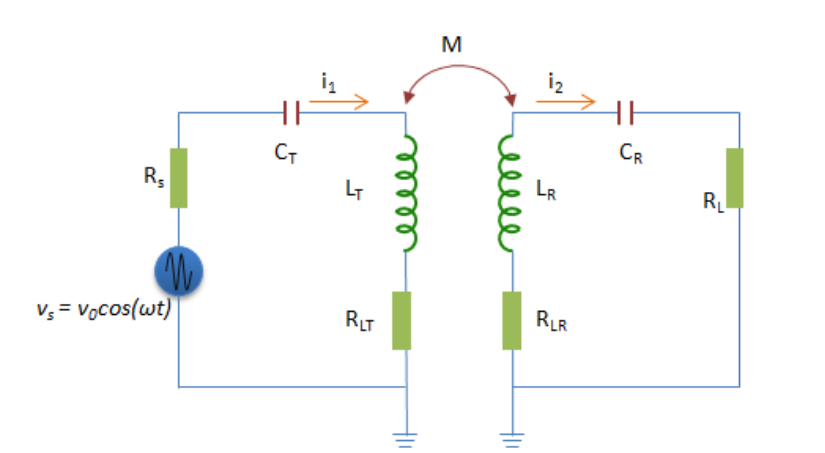
\includegraphics[scale=0.3]{EquivalentcircuitofinFigur1.png}}
\caption{A complete sound packet.}
\label{fig}
\end{figure}

$$ P_{R}(\omega)=P_{T}Q_{T}Q_{R}\eta_{T}\eta_{T}(r_{T}^{3}\mu_{0}\mu_{R}r_{R}^{3}\mu_{0}\mu_{R}\pi^{2})/(r_{T}^{3}+d^{2})^{3}.$$

where 

$P_{T}$    :Transmission power,
           
$Q_{T},Q_{R}$           : Q-factors of transmitter and receiver antenna,
          
$\eta_{T},\eta_{R}$    : Efficiency of transmitter and receiver antenna,              
                      
$r_{T},r_{R}$            : Efficiency of transmitter and receiver antenna,
           
$\mu_{0}$                          : Radii of transmitter and receiver antenna coil,
           
$\mu_{r},\mu_{R}$                        : Permeability of air (=1),
           
$D$           : Relative permeability of transmitter and receiver antenna coil core, and Distance between transmitter and receiver antenna.

An NFC system basically consists of three components as shown in Figure 5. This is the typical case when an NFC phone reads an NFC tag and communicates with the backend server [3-5]. In some cases, NFC tag can be another NFC phone or also there would be no need to contact backend server [6-7]. In essence, an NFC mobile system consists of an NFC tag, an NFC chip embedded mobile phone
and a backend server.

The security of NFC can be confirmed to some extent. However, as it is a wireless technology, some security issues are inevitable [12-13]:

\textbf{1,Eavesdropping :} Through eavesdropping, an attacker can receive the transferred information using a suitable antenna.For NFC attack, this antenna should be close enough. But, there is no solid analysis on accurate range
for possible attack as it depends on attackers' antenna parameters. It is to be worth noted that NFC provides no defense mechanism against eavesdropping. In literature [8], it is discussed that eavesdropping in NFC is difficult if a device is working on passive mode. Hence, operating on passive mode could be one of the countermeasures against eavesdropping. However, it is not practical for an NFC device to always operate on passive mode. Therefore, eavesdropping can be avoided by establishing a secure channel between the devices.

\textbf{2,Data Modification}
If the attacker has enough knowledge of the transmission, such as the mode of operation, the modulation technology used, etc., then different RF fields can be used to tamper with the data. This attack can be further divided into the following three types[14]:

\textit{1) Data Alteration:} The attacker sends a valid but modified data to the receiver.

\textit{2) Data Insertion:} The attacker inserts its data shortly before the receiver acknowledges the transmission.

\textit{3) Data Destruction:} The attacker destroys or blocks the transmitted data so that it cannot be read by the receiver (DoS attack).

For data modification, the attacker should generate his own RF field based on the modulation and transmission techniques used by the NFC device. This is very difficult from the perspective of the attacker. In addition, NFC devices can operate in full-duplex mode. This means they can check the RF field generated by the attacker to avoid collisions.

\textbf{3,Man in the middle Attack:}The attacker receives the signal from the transmitter and modifies or modifies the data and sends it to the receiver and vice versa. Although this is a big issue in large-scale network security, NFC is very difficult or almost impossible because the transceiver can detect the radio field during communication and can know the unknown RF field or collision.

However, the three major mainstream payments using NFC payment now are Samsung Pay, Apple Pay, and Google pay. Its essence of TOTP technology, in the middle of the attack, will reveal a great security risk. These are mentioned in section 5.

\textbf{Lost devices and abandoned connections}
NFC-enabled mobile devices are easily lost. However, they contain important information such as credit cards and personal data. Therefore, anyone who finds missing devices can use it just like using a lost credit card. In this case, manual security in the mobile device is the only solution, such as secure access to the phone through some PIN code or personal identification number.

On the other hand, short NFC communications can be abandoned without closing after use. These abandoned connections can be used by attackers for a variety of purposes. Therefore, communication timeout techniques should be implemented to avoid such attacks.

\begin{figure}[htbp]
\centerline{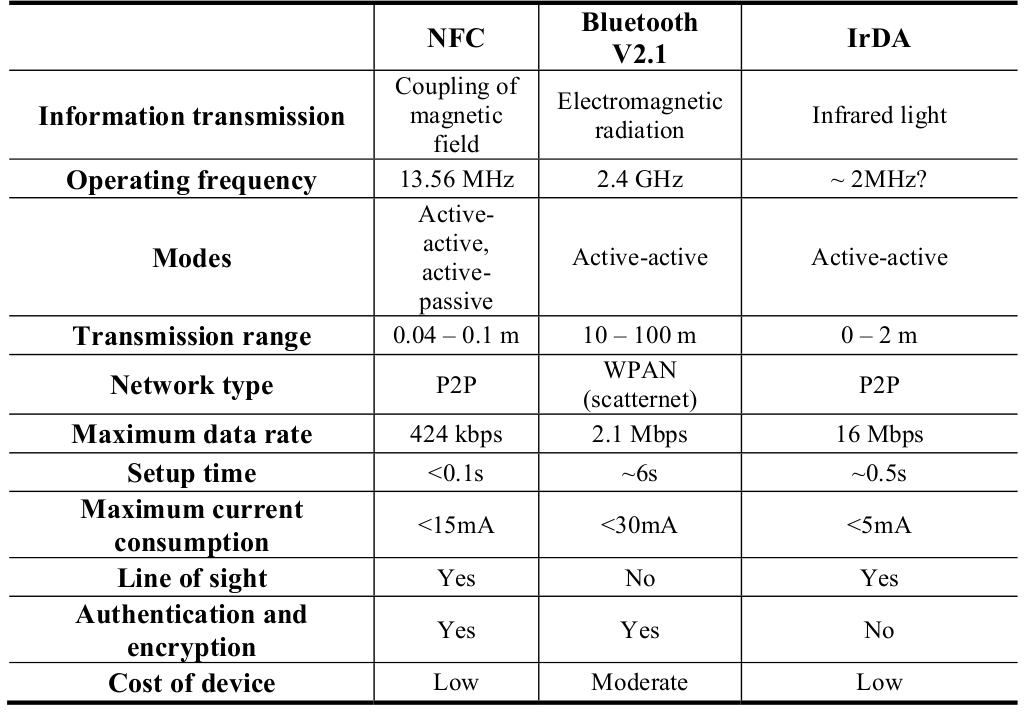
\includegraphics[scale=0.25]{ComparisonoNFCandotherPANtechnologies.png}}
\caption{Comparison of NFC and other PAN technologies}
\label{fig}
\end{figure}

An NFC system basically consists of three components as shown in Figure 5. This is the typical case when an NFC phone reads an NFC tag and communicates with the backend server [4-6]. In some cases, however, NFC tag can be another NFC phone or also there would be no need to contact backend server [7-8]. In essence, an NFC mobile system consists of an NFC tag, an NFC chip embedded mobile phone and a backend server.

An NFC tag is generally embedded in items (from which it can be read) such as smart posters [4],POS, electronic devices, etc. It is a small chip usually hidden behind a sticker with NFC logo on it in order to make users aware of its existence. These tags usually contain small data based on their applications such as uniform resource identifiers (URIs), contact information, authentication credentials, valuable information, etc.

NFC chips are embedded within mobile hand-sets enabling them to read NFC tags. Mobile phone industry has shown several NFC mobile phones manufactured in last few years. It is also possible to include NFC chip within Subscriber Identity Module (SIM) card or even in micro SD cards. Therefore, hand-sets manufactured without NFC chips from industry can also be made ‘NFC-equipped’ by inserting NFC-SIM or NFC-micro SD cards.

The NFC phones have several applications installed to utilize NFC capabilities based on the implementation of the system. It can also emulate existing cards such as credit cards, point cards, identity cards etc to give experience of these traditional schemes within a single mobile phone. Hence, a user is give experience of having 'everything' within their mobile device.

NFC phone could communicate to the backend server through different mobile communication technology. Service provided by the backend server might vary according to applications. For an instance, it could be a simple web page for reserving movie ticket, issuing receipts, or highly secure financial transaction service. Therefore, communication between handsets and backend server needs to implement secure connection.

Similar to RFID, NFC can also communicate on active/passive mode [9]. This means that an active NFC device is the one with power supply and generates radio field. The NFC device working on passive mode gets power supply through the active devices radiation. On the other hand, both the NFC devices can also work in active/active mode where both the devices are active devices with their own power supply. Generally, NFC can operate on three modes [4].

An NFC enabled phone acts as a tag or a kind of contactless card in card emulation mode. These tags can be read by existing traditional card readers. For an instance, it can be used as an identity card at school or office to unlock door, activate personal devices such as PC, printers, etc. Also, most
common usage would be to emulate credit cards or points cards which can be used at POS terminals for
payments.

An NFC has a predefined data format called NDEF data format. When an NFC phone is in read/write mode, it can read from or write data to supported tag types. Particular example usage of read/write mode is to access URI from smart posters, download short manuals of electronic devices, check out bus - arrival information at bus stops, etc.

The peer to peer mode adds quality functionality to NFC phones. In this mode, two NFC phones can exchange data with each other when brought to close proximity. For an example, two business partners can transfer their virtual business cards with each other by bringing their NFC-enabled phones close to
each other. Another popular usage is for connection handoff to other standard technology; NFC connection can be used to set-up Bluetooth pairing or Wi-Fi setup. After successful setup, the handset can use the Bluetooth or Wi-Fi connections.
\begin{figure}[htbp]
\centerline{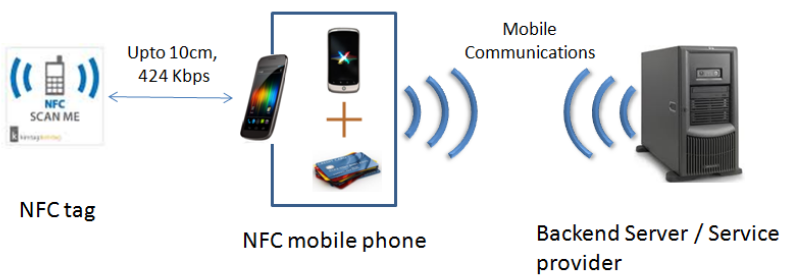
\includegraphics[scale=0.3]{NFCinactive.png}}
\caption{NFC in active/passive mode}
\label{fig}
\end{figure}


\subsection{MST}
Magnetic Secure Transmission (MST) is a technology that can transmit magnetic signals that simulate the magnetic stripe on a traditional payment card. The MST sends a magnetic signal from your device to the reader of the payment terminal (simulating the physical card swiping without upgrading the terminal's software or hardware). Almost all payment terminals with card readers can use MST technology. Some payment terminals may require software updates. Simply select a card from Samsung Pay and transfer the payment information by moving the device within one inch of the payment terminal. Your transaction and payment information will use tokenization for privacy and security. MST is more secure than using traditional payment cards and is as secure as using Near Field Communication (NFC) payments.

The technology was developed and patented by LoopPay. Samsung previously acquired the company to deploy its Samsung Pay service.The biggest highlight of Samsung Pay and Apple Pay is support for magnetic stripe card payments.

Figure 3 shows the components of the payment accessory that LoopPay made for Samsung. By using AC current, the coil will generate a magnetic field.If the correct magnetic field is generated, the coil can communicate with a credit card reader.In fact, the principle of MST is to emit a magnetic field.

\begin{figure}[htbp]
\centerline{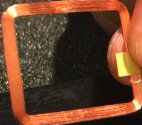
\includegraphics[scale=1]{MSTyuanjian2.png}}
\caption{token service provider}
\label{fig}
\end{figure}

However, payment security is not solved by a copper coil.The MST application has three protection mechanisms: Payment Tokenization, eSE (hardware security module) bank card information protection, KNOX, and fingerprint/password authentication.

\begin{figure}[htbp]
\centerline{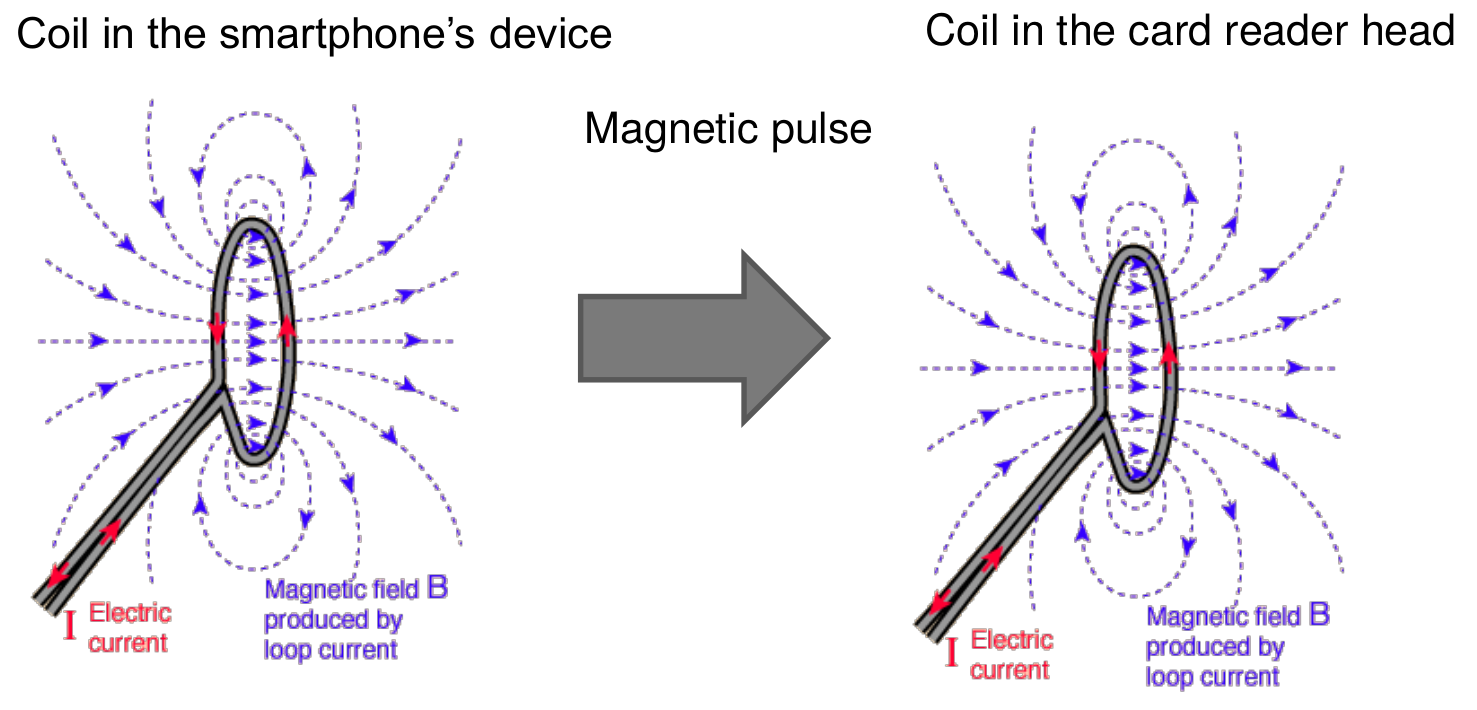
\includegraphics[scale=0.18]{Emittingmagneticpulse.png}}
\caption{Emitting magnetic pulse.}
\label{fig}
\end{figure}

For Token, the user needs to enter the card information and send it to the card organization for verification. After the card organization passes the verification, a token will be generated for this card and the token will be sent to the device. The credit card information is not directly stored on the device. Token is stored in an independent security chip (SE chip) and used to replace the bank card number. It can be understood that the Token and the bank card number are equivalent, but even if the Token leaks, the bank card information cannot be reversed. Only when fingerprint or password authentication passes can the token be read out through the MST. Token's storage and management is governed by Samsung's own KNOX security platform.High-risk behaviors such as equipment modification occur, and KNOX can invalidate sensitive data on the device.

In other words, when using Samsung Pay's magnetic card payment mode, the key technical step is how this Token is sent. The MST generates a dynamic magnetic field through an induction coil and can be changed according to the user-defined time limit. If your mobile device is within 3 inches of the reader, you will be able to identify the magnetic field.

Like a traditional credit or debit card, magnetic fields include your payment information. The magnetic field only exists when the user chooses to send the payment information, and the magnetic field will automatically disappear once the distance between the mobile device and the reader exceeds 3 inches. This means that the attacker must be very close to the payment process to steal the payment data.

Near Field Communication (NFC) allows two devices to be located a few inches apart to exchange information. NFC payments require merchants to upgrade old terminals to NFC-enabled payment terminals. Magnetic Secure Transmission (MST) Sends magnetic signals from compatible devices to the payment terminal's reader (emulates card swiping physical payment cards). The MST payment does not require the merchant to upgrade the payment terminal so that Samsung payment can be used on almost all payment terminals with a card reader. Some payment terminals may require software updates. Samsung Pay uses NFC and MST to send payment information to the terminal. Whether using NFC or MST, transactions are seamless, providing a better user experience. Both technologies are equally secure, using a unique digital card number instead of the actual payment card number. Your information is confidential and secure. Only the payment network of your bank and credit card will provide transaction information.


\subsection{Audio}

The audio protocol we are talking about today for sonic communication is generally from the technical documentation of chirp which is a novel application for "transmitting" files via voice issued by the American startup Animal Systems.

Acoustic wave transmission is a set of technical solutions that use sound to achieve fast transmission of files: Cross-platform technology is used to implement data transmission between any device that can send sound waves and receive sound waves.There are also a large number of applications in mobile payments.

\subsubsection{encoding}
The principle of the audio protocol is simple and easy to implement. Create a table with 32 characters and map each character to a frequency table. The frequency table is generated based on the music theory through the calculation of sound.Each character is represented by the pitch of one frequency, so there are 32 frequencies, 0 corresponds to 1760 Hz, 1 corresponds to 1864 Hz,..., v corresponds to 10.5 kHz, and the adjacent frequency differs by a half interval.

The audio produced by Chirp contains 20 characters. Each character is generated with a sine wave of the corresponding frequency. Each sine wave lasts 87.2 ms. If the sampling rate is 44.1 kHz, then each character is about 3846 samples. The whole audio is about 20*87.2ms=1.744s, because each character is represented by a different frequency, it sounds like music.

A complete sound packet contains 20 tones (ie 20 characters), one tone every 87.2 milliseconds. The first two bits are headers and use “hj” to notify the receiver to start receiving. The middle 10 bits are valid information bits, which are effective transmission information, that is, Key values are mapped after the frequency information. The last 8 bits are the RS check digits. The RS parity check algorithm calculates the middle 10 bits and generates 8-bit parity information.

\begin{figure}[htbp]
\centerline{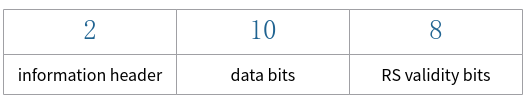
\includegraphics[scale=0.4]{yinpinwei.png}}
\caption{A complete sound packet.}
\label{fig}
\end{figure}

\subsubsection{decoding}

Chirp describes the technical details of relying on sound for data communication between a smart device, but in fact, the audio protocol of the sound wave communication can be arbitrarily designed by itself, for example, changing the sound in the chirp audio protocol to double-frequency sound, even multi-tone sound. In order to increase the information capacity per unit time, thereby increasing the transmission speed, this is all possible, as long as there is a demand for this application.

The receiver needs to record the sound and perform it and fault-tolerant processing. Its relatively high requirements on the algorithm, noise reduction and fault-tolerant processing are critical to the correct information

\section{online payment technologies}

\begin{figure}[htbp]
\centerline{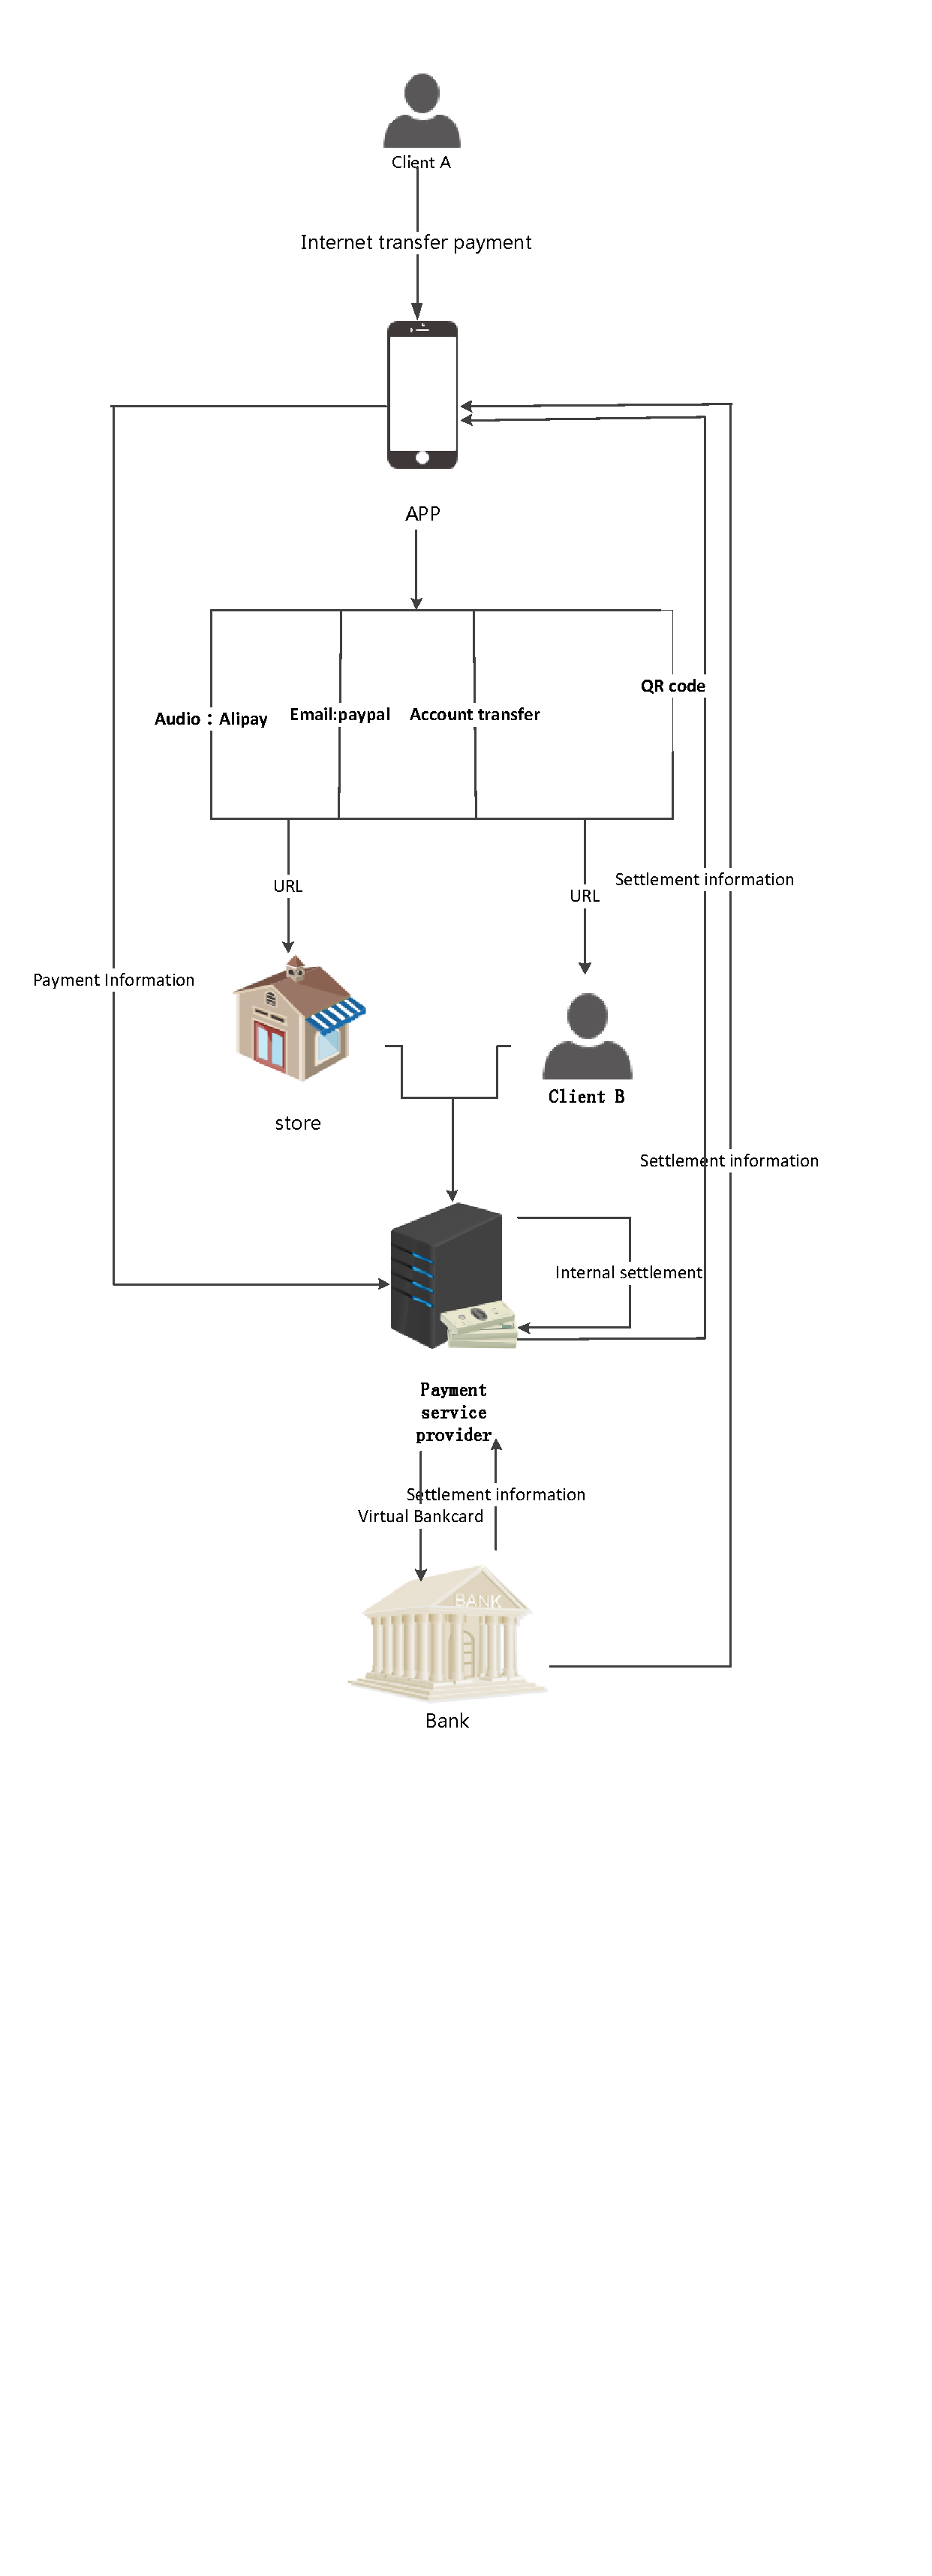
\includegraphics[scale=0.58]{zhuanzhangshifu.pdf}}
\caption{Token application process.}
\label{fig}
\end{figure}


Internet transfer payment technology, as the name suggests, is a transfer payment via the Internet.Different from the PC terminal, the network transfer payment at the mobile terminal needs to pay for the support of the client's app.

Network transfer payment technology is mainly based on the security of tokenization technology.



\subsection{scan the QR code}
In the scan code payment scenario, the QR code is actually a url with some parameters. The scan code will initiate the transfer. The two-dimensional code is actually only an account medium, a data storage body, which itself is not the result of the payment innovation. The existing various QR code payment only replaces the data carrier of the original payment means with a two-dimensional code. Similar chip content with bank cards. Is an account of the embodiment. 
\begin{figure}[htbp]
\centerline{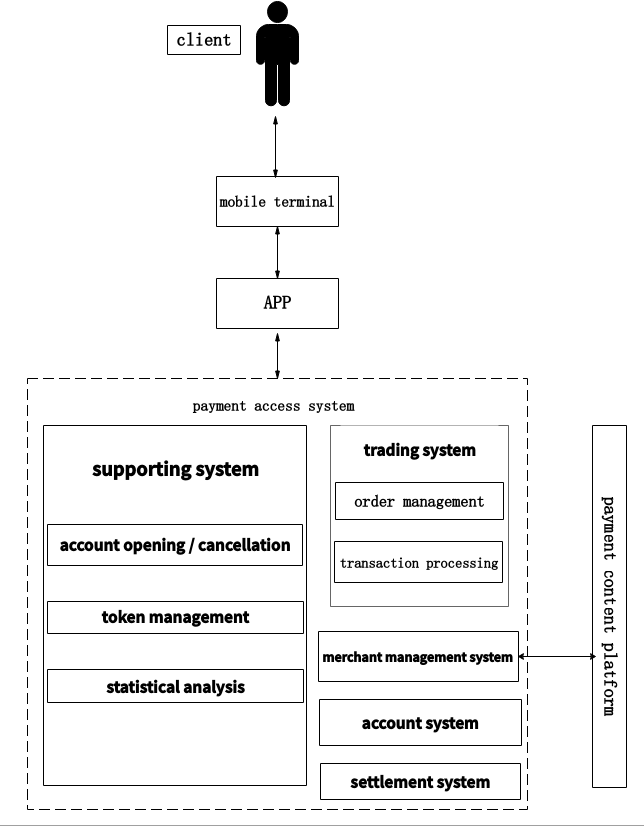
\includegraphics[scale=0.44]{erweimazhifu.png}}
\caption{App payment.}
\label{fig}
\end{figure}
\subsection{Through email}

\section{offline payment technologies}
Offline payment is a payment method which the most prominent feature is that the paying party do not need connecting to the Internet, which means only one party need communicate with the payment server.It is widely welcomed due to its ease of use. In China today, this type of payment method can be seen everywhere, from large shopping malls to small supermarket chains. Even in the underground shopping malls with poor network signals, the surrounding areas of the city, and tourist attractions in the mountains, as long as a mobile phone in hand, you can pay for you. 

Off-line payment is mainly provided by two major technologies, one mainly provided  by large-scale payment service providers such as Alipay, Tencent, UnionPay, Wal-Mart, and Amazon. It mainly binds the bank card to the account of the corresponding payment provider and uses the TOTP technology to generate the payment password and use the account number to pay. Another source is mainly provided by large mobile terminals or system providers, such as Apple, Samsung, and Google. It mainly binds the bank card to the mobile phone terminal and simulates the bank card payment method and pays for direct connection to the bank.

Figure 15 shows the entire process of offline payment from client to bank, including TOTP payment represented by Alipay and analog bank card payment represented by Samsung.

First look at the former, after the TOTP is generated by the mobile phone, the QR code or audio is used as a carrier to the store. The store transmits the TOTP plus payment information to the server of the payment service provider, decodes the TOTP and completes the settlement. At this time, the payment provider The money in the customer's account in the database is transferred to the store's account.
\begin{figure}[htbp]
\centerline{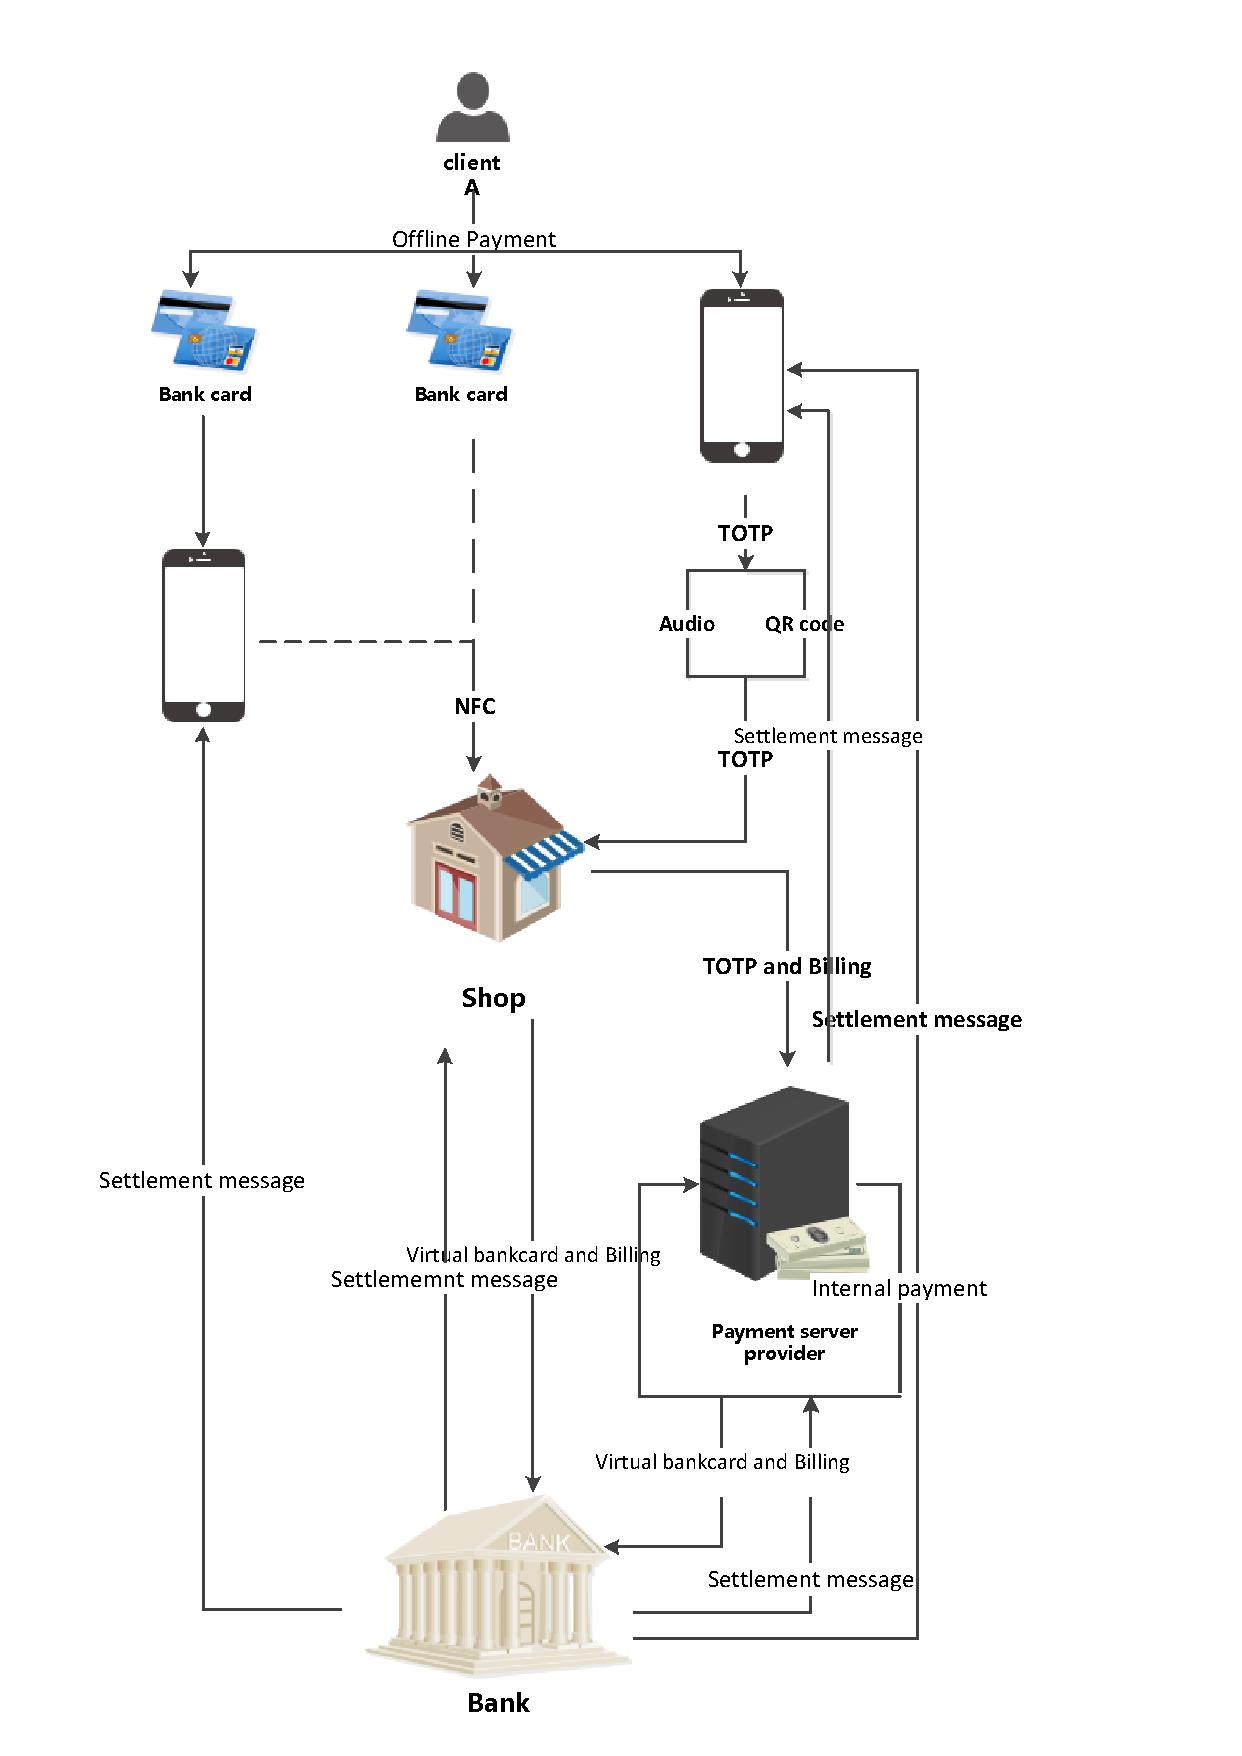
\includegraphics[scale=0.68]{offline.pdf}}
\caption{Offline payment.}
\label{fig}
\end{figure}
\subsection{Time-Based One-Time Password:The key to offline payment}
one of the technical prototypes of the off-line payment is a one-time password (OTP) widely used in the industry. Products using this technology include Alipay and WeChat, as well as hardware equipment such as bank U shields and game tokens.

Regardless of Alipay or WeChat, they scanned the payment using 18-digit digitally-generated barcodes and QR codes. This 18-digit number is the payment password. 


\subsubsection{HMAC(Message Authentication Code Algorithm Based on Hash Function)}
Algorithm formula:
$$HMAC(K, m) = H((K^{\prime} xor opad) || H ((K^{\prime} xor ipad) || m)) $$

$\bullet$ H:hash functio4;

$\bullet$ K:shared secret key;

$\bullet$:$K^{\prime}$ calculated by K(key) (The hash function of this scheme is SHA-1, MD5, RIPEMD-128/160, and the size of $K^{\prime}$ is 64 bytes, followed by 0);

$\bullet$ xor;

$\bullet$ opad:outer HASH padding value, 0x5c5c5c.... Length equal to K’ $K^{\prime}$;

$\bullet$ ipad:inner HASH padding value, 0x363636.... Length equal to  $K^{\prime}$;

$\bullet$ m:a message input;

$\bullet$ $||$:Indicates connection.

\subsubsection{HOTCP(HMAC-based One-Time Password)}
Algorithm formula:
\\
$HOTP(K,C) = (Truncate(HMAC(K,C))\&0x7FFFFFFF) 
\\mod 10^{d}$

$\bullet$ C:counter;

$\bullet$ Truncate:after processing will get a 32bit unsigned integer;

$\bullet$ A d-bit numeric password is obtained with a d-squared modulus operation of 10.
\subsubsection{TOTP(Time-Based One-Time Password)}
Algorithm formula:
\\
$$TOTP = HOTP(K, TC)$$

$\bullet$ $TC=f((unixtime(now) − unixtime(T0)) / TS)$;

$\bullet$ T0:The time step to start the calculation;

$\bullet$ TS:Time Step.
\\
\\
After the terminal installs the client and starts the application for the first time, the server can generate a unique token and the device ID corresponding to the token.

$\bullet$ Token: The seed used to generate the OTP code.

$\bullet$ Device ID: Used to uniquely identify the terminal.

After sending the token and the device ID to each terminal, the server needs to store the mapping relationship between the token and the device ID.


The terminal calculates the dynamic password by using the pre-stored token and the current time as input values of the first preset algorithm.

The first preset algorithm may be an arbitrarily formed irreversible algorithm
                           
                           $1$, time synchronization algorithm (TOTP);
 
                           $2$, event synchronization algorithm (HOTP);

                           $3$, challenge response algorithm (OCRA);

Alipay and moust of payment server provider now mainly uses TOTP technology




The first information can be any of the following:

1, dynamic password: such as: 123456.

2, the combination of dynamic password and current time value: such as: 123456 (dynamic password) 20160503110232 (current time value)

3, device ID and dynamic password:

4, device ID and dynamic password + current time value.

The first information including the above-mentioned dynamic password is used as the input value of the second preset algorithm, and the second information is calculated.

The second preset algorithm is an irreversible algorithm such as: HMAC, MD5, or HMAC-SHA algorithm.

 second information is generally obtained with the token and the first information as input values

1, find the corresponding token with the device ID of the authentication password

2, using the token and the first default algorithm to verify the dynamic password.
The trusted dynamic password list is first calculated (the trusted dynamic list includes multiple trusted dynamic passwords).
If it is found that a certain trusted dynamic oral delivery is consistent with the above-mentioned dynamic password, the dynamic password verification passes.

3, using the first information and the second preset algorithm to verify the second information




10: device ID

20: Dynamic password

30: second information

\begin{figure}[htbp]
\centerline{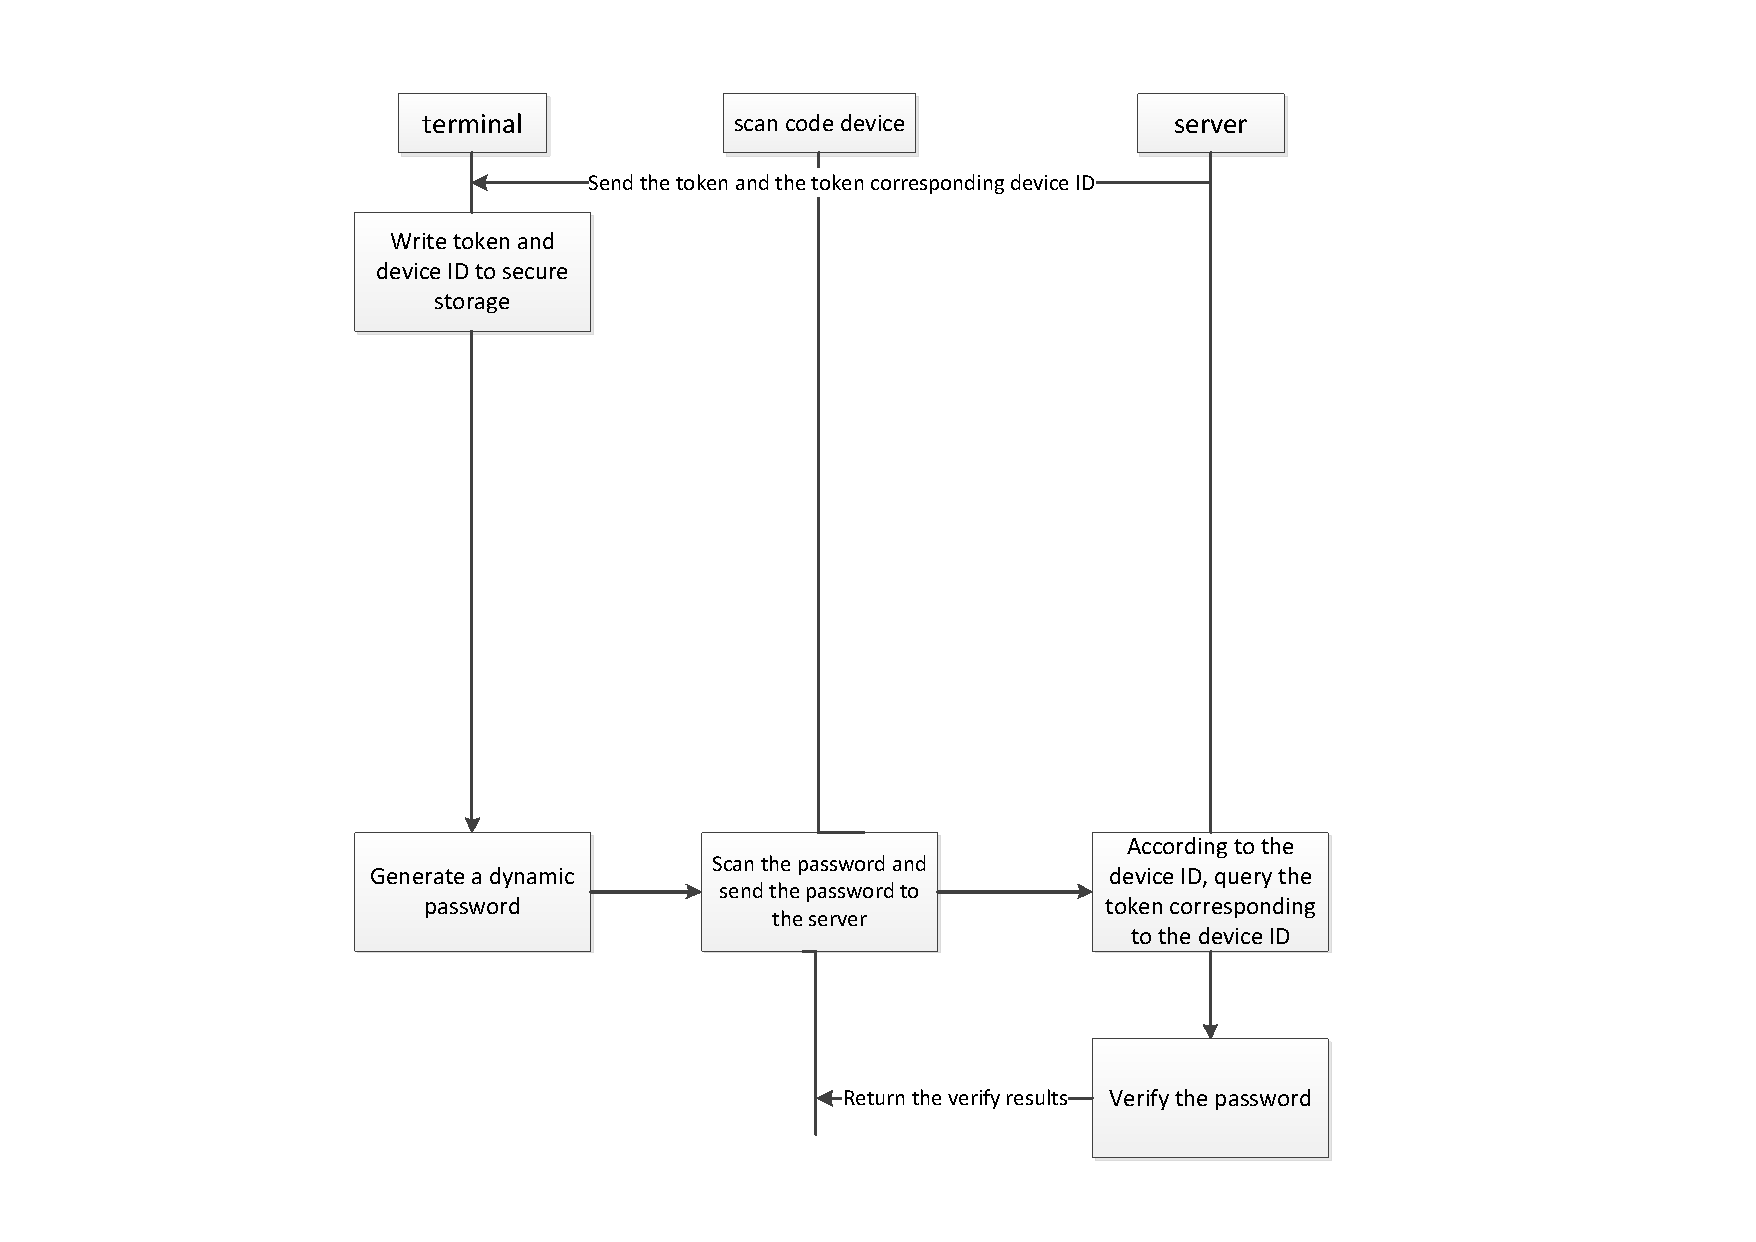
\includegraphics[scale=0.62]{TOTP2.pdf}}
\caption{Time-Based One-Time Password.}
\label{fig}
\end{figure}

\begin{figure}[htbp]
\centerline{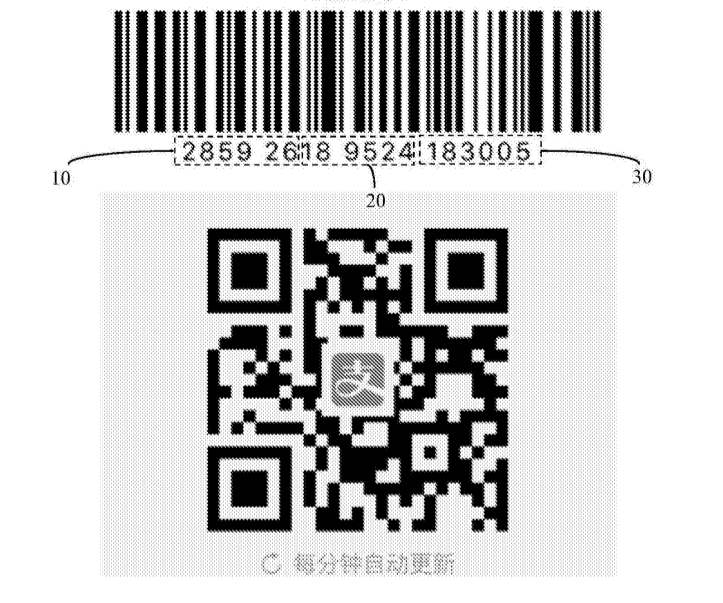
\includegraphics[scale=0.6]{QRcode.png}}
\caption{Offline payment.}
\label{fig}
\end{figure}

\begin{figure}[htbp]
\centerline{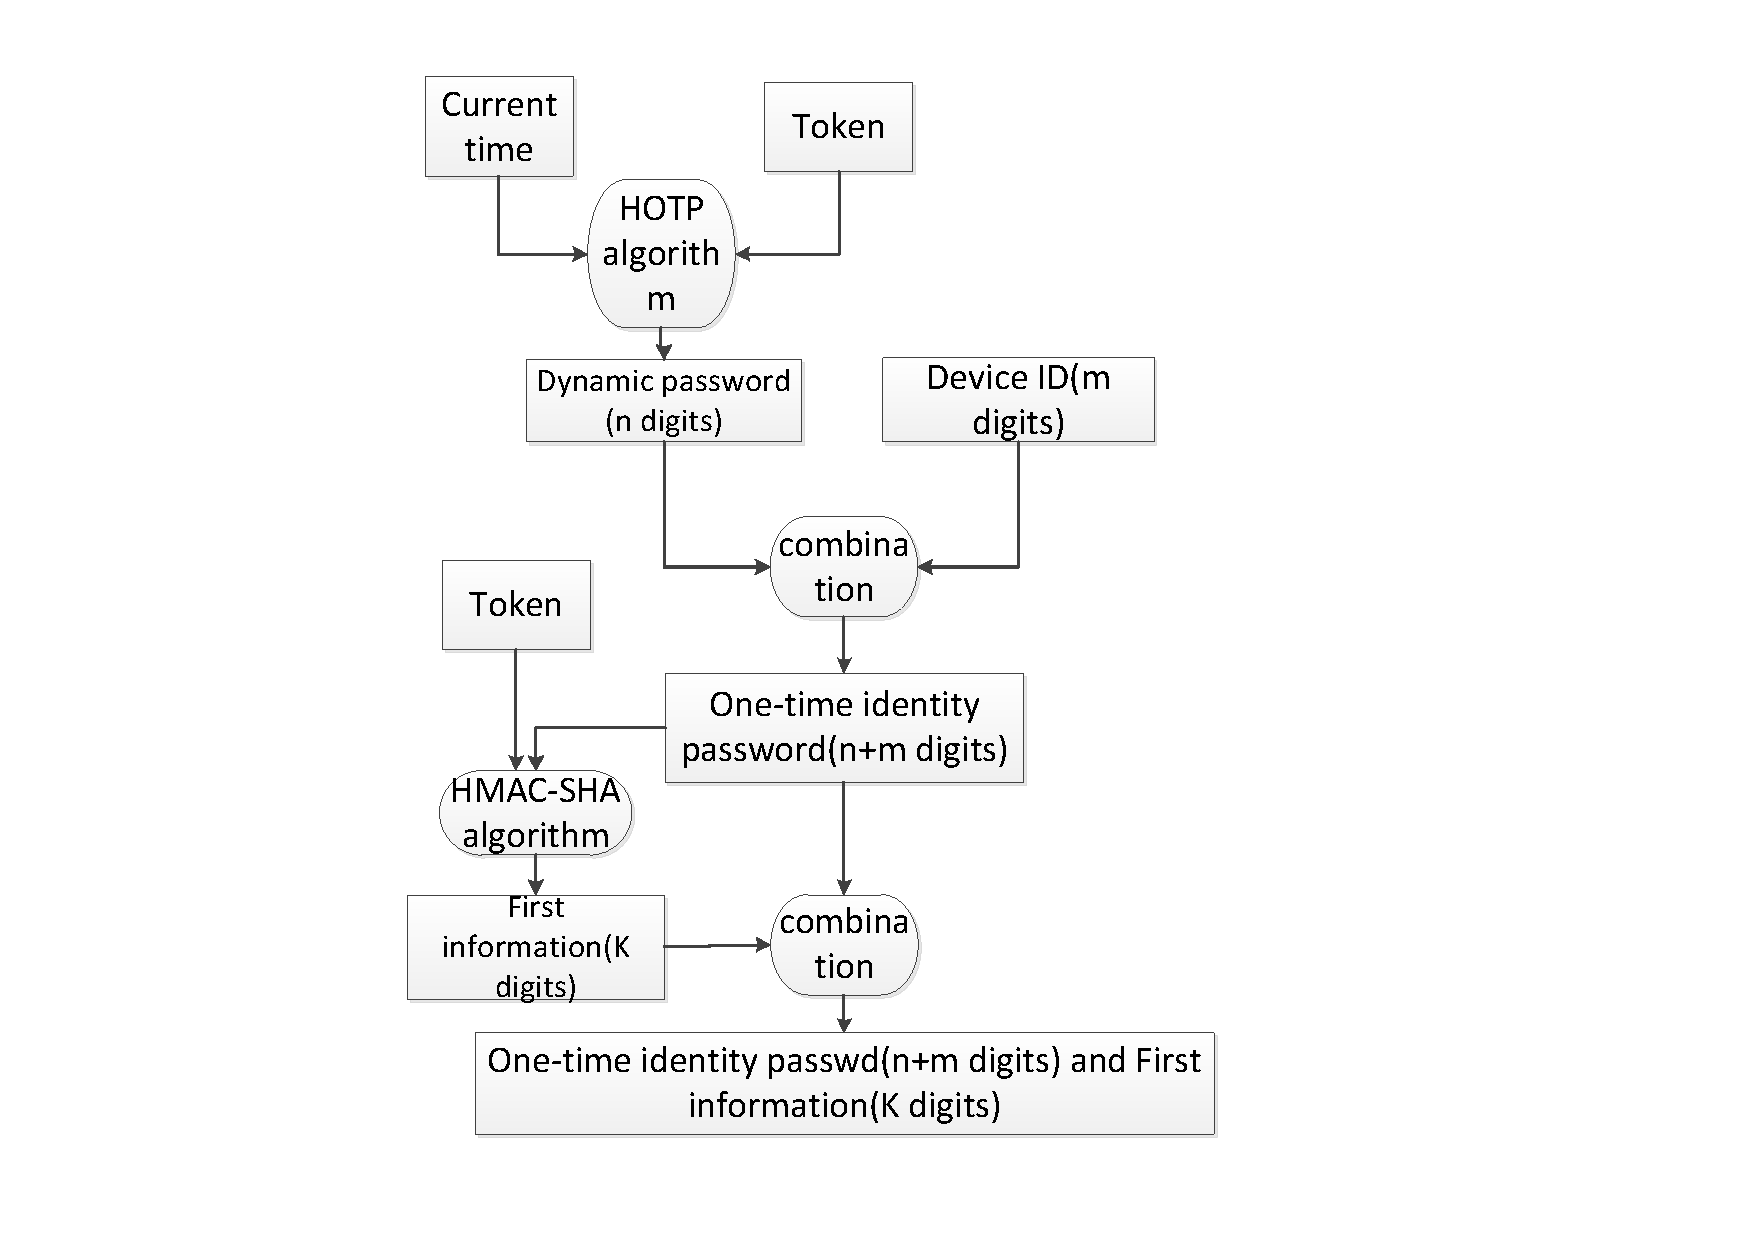
\includegraphics[scale=0.65]{TOTP.pdf}}
\caption{Time-Based One-Time Password.}
\label{fig}
\end{figure}


\subsection{IC card and its imitation payment}
IC card credit card payment is the main portable payment method before mobile payment. Especially in Europe and the United States, it has become a payment method that many people have become accustomed to. Therefore, Samsung, Apple, Google and other large European and American Internet companies have taken a different path from companies such as Alibaba and Tencent when they entered the payment industry.

Different from the use of the two-dimensional code, audio, and other means. They work directly with banks and  are committed to using mobile phones to simulate IC card payments which hope to have a swipe experience on the mobile phone.

\subsection{bank card}
The bank card is divided by the interface and can be divided into:

\textbf{magnetic card;}

\textbf{IC card (chip card).}
\subsubsection{magnetic card}
A magnetic card is a card-like magnetic recording medium that uses magnetic carriers to record characters and digital information for identification purposes or other purposes. The magnetic card is made of high-strength, high-temperature-resistant plastic or paper-coated plastic, and can be damp-proof, wear-resistant and have certain flexibility. It is easy to carry and uses more stable and reliable. For example, the bank card we used before is the most common magnetic stripe card.

The magnetic stripe card is a veteran of the card industry. It has the longest usage time and the largest number of uses. With the development of informatization and electronic technology, magnetic stripe cards have gradually faded out of the stage of history due to the disadvantages described above.

\subsubsection{IC card}
An integrated circuit card (IC card) is also called a smart card, an intelligent card, a microcircuit card, or a microchip card. It embeds a microelectronic chip into a card base conforming to the ISO 7816 standard in the form of a card. The communication between the IC card and the reader can be either contact or non-contact. According to the communication interface, the IC card is divided into a contact type IC card, a non-contact type IC, and a dual interface card (having both a contact type and a non-contact type communication interface).

Because of its inherent information security, portability, and relatively standardization, IC cards are increasingly used in identity authentication, banking, telecommunications, public transportation, and yard management, for example, second-generation ID cards, and banks. Electronic purses, telecommunication SIM cards for mobile phones, bus cards for public transportation, subway cards, parking cards for parking fees, etc. all play an important role in people's daily lives.

IC card is another kind of information carrier after the magnetic card. The IC card refers to an integrated circuit card. A commonly used bus card is a kind of IC card. Generally, a common IC card uses radio frequency technology to communicate with a card reader supporting an IC card. There is a difference between the IC card and the magnetic card. The IC card stores information through the integrated circuit in the card, and the magnetic card records information through the magnetic force in the card. IC cards are generally higher in cost than magnetic cards, but have better confidentiality.

The subdivision of chips can be divided into 

\textbf{contact card:}Contact: only support contact transactions, transactions need to plug into the POS machine

\textbf{non-contact card:}Non-contact: only support non-contact transactions, trade on the POS machine, usually non-contact IC is buried in the card, the surface can not see.

\textbf{dual interfaces card.:}The dual interface means that the IC card supports both interfaces. Therefore, only when the bank card is an IC card that supports non-contact transactions, it is possible for the NFC terminal to read the card information.







\section{Mobile phone emulate IC card}
With the gradual deployment of Android Pay, Apple Pay and Samsung Pay, mobile payments have returned to the public eye and the comparative articles on several types of payment have not been uncommon in recent days. This article mainly discusses the similarities and differences between several payment methods from a technical point of view.
\\

Apple Pay and Android Pay each serve as a system-level payment application (Apple Pay by iOS, Android Pay by Android), not only play the role of application, but also has a God perspective, as a system feature for other applications developers A unified payment gateway. In other words, other shopping and service applications can invoke APIs of Apple Pay or Android Pay in the development code to charge consumers, for example, purchasing a movie ticket. Before the application is almost always linked to VISA or MasterCard online payment allows users to fill in the cardholder name, card number, expiration date, code and other safety information, each time you have to fill in the shopping (the site should not and can not be saved), or combined with OTP (one-time password) certification, This is a hassle and a safety hazard (previously PC-based cookies were hacked, or consumer websites saved user-card information, such as previous Ctrip, resulting in theft of credit card information); application developers can now call Pay, allowing users to choose their own credit card has been added to pay, users do not need to fill in a form, a key shopping, the real charge to pay to do.\\

Relative to the online payment (in short, that is connected with the Internet, the payment of data through the network transmission), offline payment is a physical payment, you need a terminal device chargeback, in most cases, POS machines. In order to replace the traditional credit card with credit card spending, NFC + Pay way allows consumers to use a cell phone, rather than a variety of cards for "flash" consumption. Pay only needs the POS machine to support NFC without any other modification. Therefore, offline entity merchants accept this payment method exactly as the acceptance of non-connected bank cards such as MasterCard Pay Pass, Visa Pay Wave, China Union Pay Flash Quick Pass , There is no promotion barriers, but also to speed up the deployment of wireless POS machines coupled with a heavy weight.

\subsection{sumsung pay}
Samsung Pay uses NFC and MST technologies. 

Samsung Pay uses both NFC and MST to send payment information to the terminal. The transaction is seamless, whether using NFC or MST, allowing for a better user experience.

Both technologies are equally secure, using a unique digital card number in place of the actual card number. The information is kept private and secure, and only the bank and the card's payment network will have information on the transaction。

Samsung's payment technology also uses TOTP technology and virtual bank card technology. The following steps can be known from Fig 21:

\textbf{1, }The client first submits bank card-related information on the app. Samsung takes them to the bank or card organization in exchange for a virtual silver card and secret value and binds it with the user account. In addition to being stored on the server, it is also stored in the KNOX of the client's mobile phone.

\textbf{2, }Combine the virtual line card with the secret value and add the TOTP algorithm to get a one-time payment password. The following is a guess. When the payment is made again, the first 6 digits and the last 4 digits of the password are the same as the virtual bank card. The middle 8 digits are TOTP passwords.

\textbf{3,}The payment password using MST or NFC encoding, and simulate the physical bank card payment method in pos credit card. The payment password and the pos machine ID are transmitted to the bank server via the payment network.

\textbf{4,}The bank server obtains the virtual bank card by decrypting the TOTP, and obtains the real bank card through the de-tokenization technology. Finally, the bank card is used for real payment, and the payment completion information is returned to the Samsung server.

Samsung's MST payments and NFC payments are analog bank card payments. Not only that, S and C will be displayed behind the pos card number on the pos machine.

In fact, this means that the physical card swiping method. S means the media representing the card is a magnetic stripe. I means that use the intergated chip. C and Q are the non-contact transactions.

It can be concluded that Samsung's payment, while simulating the physical card payment on the surface, essentially uses the core technologies of mobile offline payment, namely, tokenization and TOTP.

\begin{figure}[htbp]
\centerline{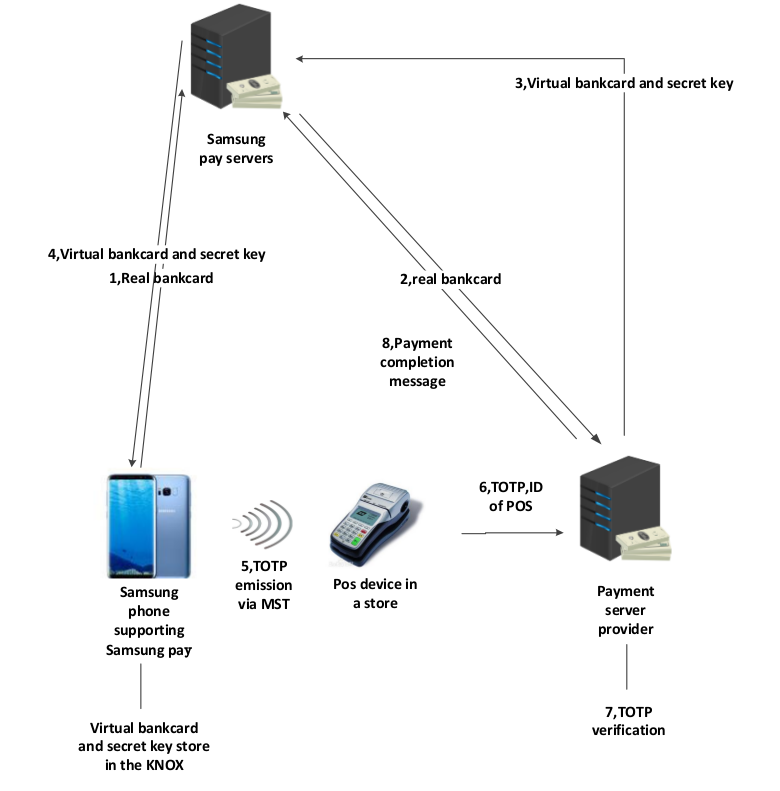
\includegraphics[scale=0.35]{sanxingMST2.png}}
\caption{samsung pay service architecture.}
\label{fig}
\end{figure}

\begin{figure}[htbp]
\centerline{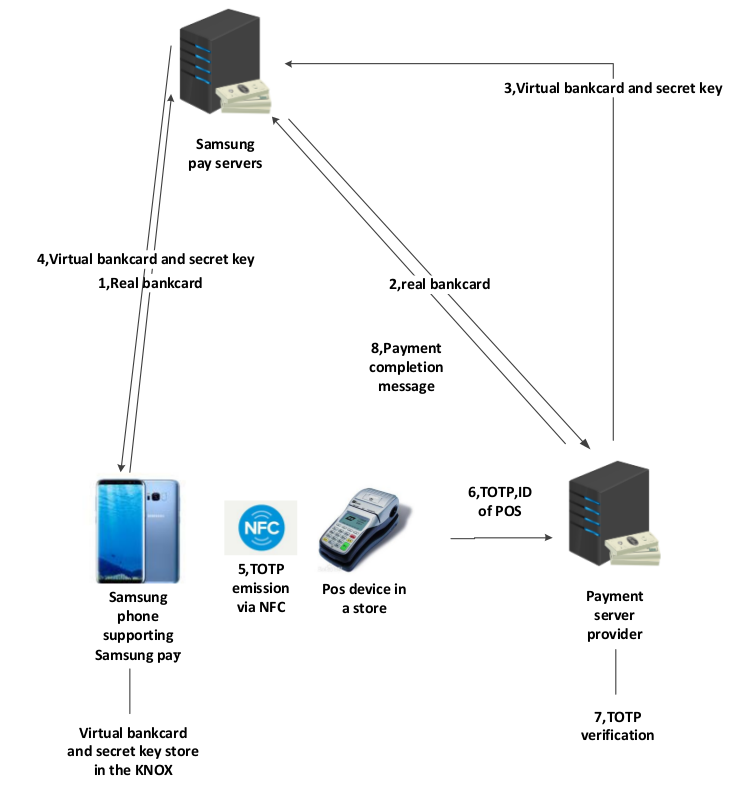
\includegraphics[scale=0.35]{sanxingNFC2.png}}
\caption{samsung pay service architecture.}
\label{fig}
\end{figure}

\subsection{google pay}
On February 20, 2018, Google announced that it has integrated Android Pay and Google Wallet, officially launched a new payment service Google Pay

\subsubsection{Android Pay}Android Pay is a mobile payment service launched by Google in 2015. It is based on the foundation of Google's electronic money package. It allows users to store credit or financial cards in mobile phones and use Near Field Communication (NFC) to transmit them. Card information to complete the payment process to replace the past credit card payment methods, while the original Google e-money packs still exist, mainly supporting network-based Play Store shopping and some application-based point-to-point payments.

The hardware limitation of using Android Pay is not severe. As long as the system is Android 4.4 or higher, and the built-in NFC chip, Android Pay can be used. In other words, as long as this condition is met, not only the mobile phone, but also the Android tablet can With Android Pay.


NFC technology has been around for more than a decade and has been called promising mobile payment technology for the past few years. But even today, NFC-enabled mobile phones are increasingly becoming the standard for smartphones, and NFC-based mobile payments have not formed widespread acceptance among consumers. One important reason is that everyone is rushing to control the Secure Element of NFC technology. The security element, as the name implies, is to ensure the security of property information. Controlling this can control the cost of each transaction. SE has led to endless battles between financial institutions, OEMs and operators. There is no way to unite them, which makes NFC mobile payment development slow.

\begin{figure}[htbp]
\centerline{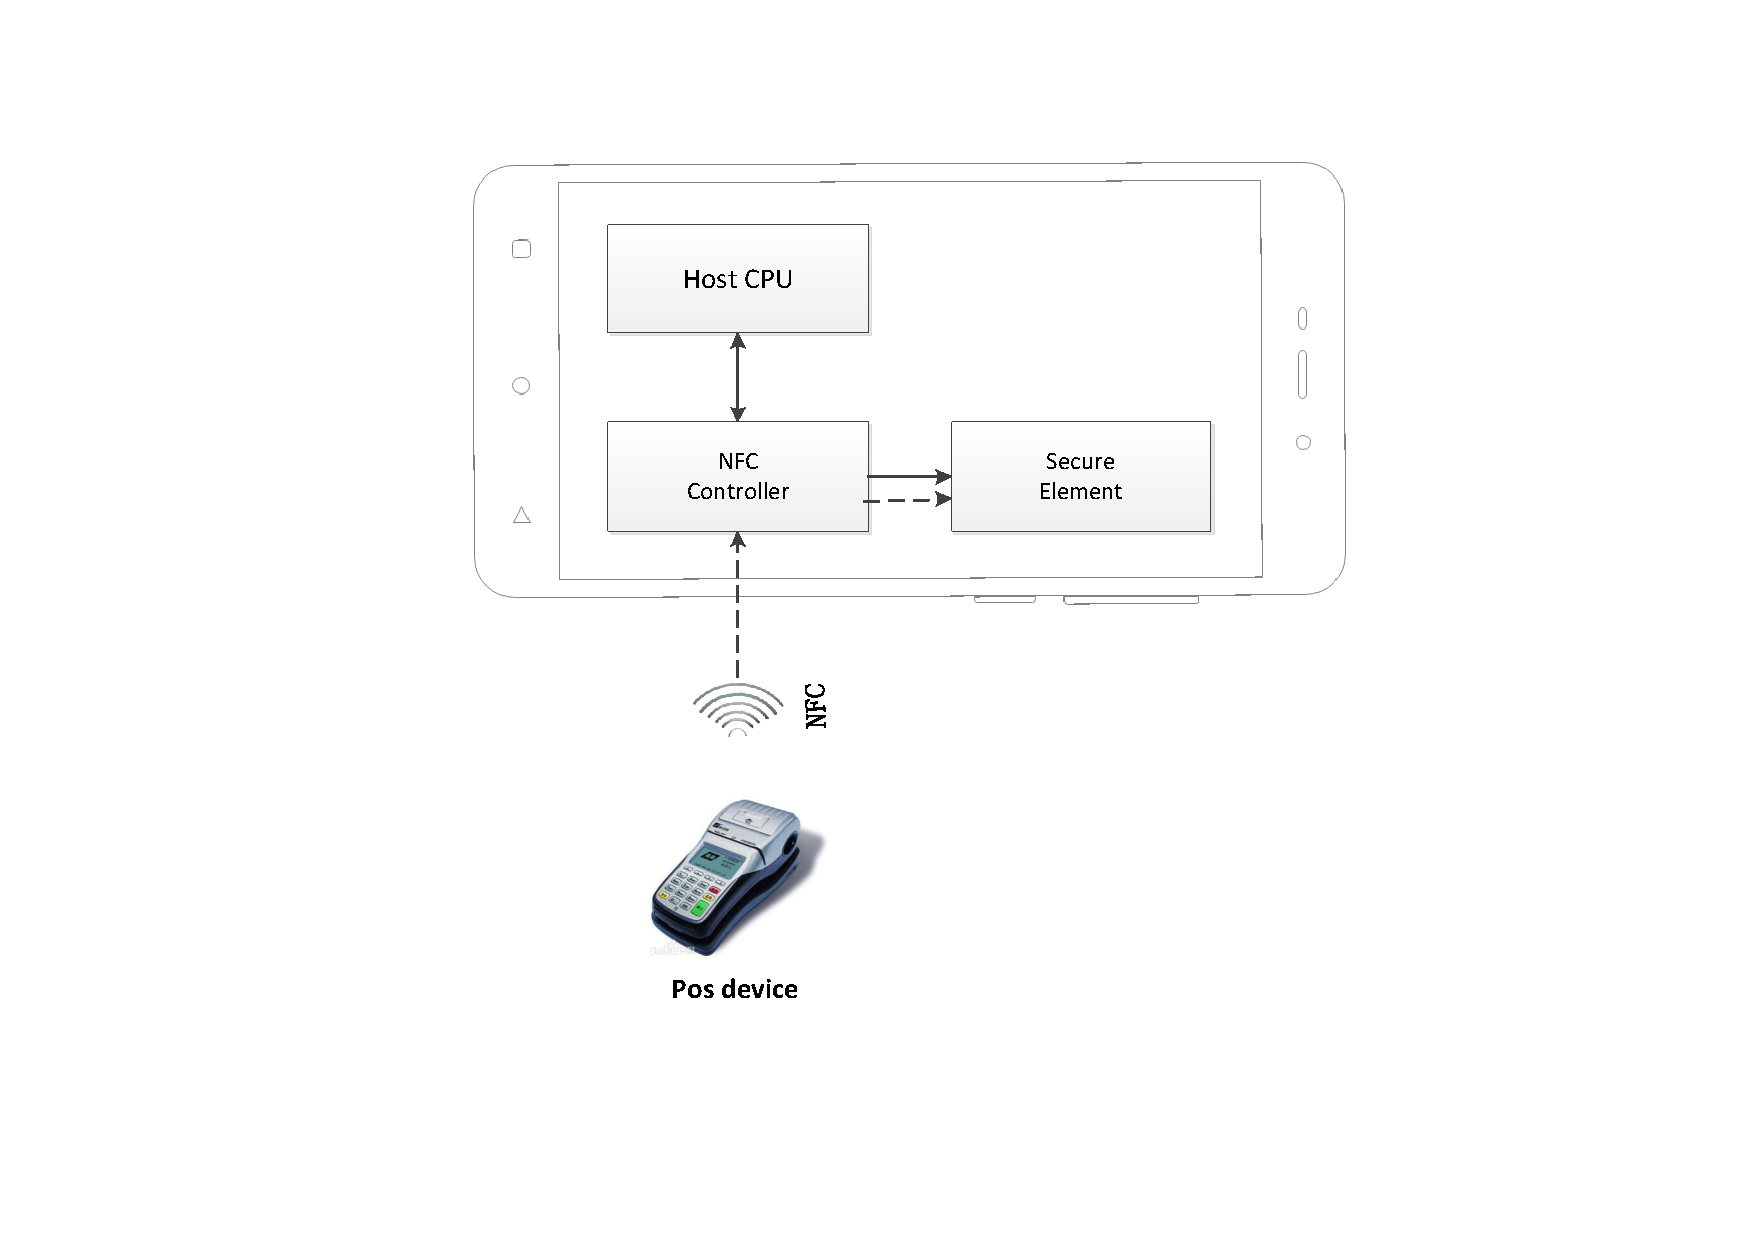
\includegraphics[scale=0.6]{NFC_se.pdf}}
\caption{NFC card emulation with a secure element.}
\label{fig}
\end{figure}


\subsubsection{HCE(host-based card emulation)}

There are two ways to implement card emulation on an NFC-enabled mobile phone: one is hardware-based, called virtual card mode; the other is software-based, called host card mode ( Host Card Mode).

In the virtual card mode, the security module SE (Secured Elemen) needs to be provided. The SE provides secure storage of sensitive information and provides a secure execution environment for transactions. The NFC chip acts as a contactless communication front end, forwards the commands received from the external reader/writer to the SE, and then processes them by the SE and replies via the NFC controller.

In the host card mode, there is no need to provide the SE. Instead, the SE function is performed by an application running in the mobile phone or a server in the cloud. At this time, the data received by the NFC chip is sent by the operating system or the application in the mobile phone, or The interaction is done through the server that the mobile network sends to the cloud. Both methods are characterized by the limitation of the built-in SE of the mobile phone. The beauty of this standard is that it does not require the entire industry to fight in order to control the safety elements.

\textbf{NFC standard support for Android:}

The NFC standard provides support for many smart card communication protocols, and the Android 4.4 system also supports many contactless smart card protocols including mainstream smart card applications. Therefore, using NFC mobile phones and HCE applications, it is possible to easily simulate different types of smart card applications. .

Many NFC reader terminals on the market also support these protocols, including an NFC-enabled Android device as the reader itself. This way we can deploy an end-to-end NFC solution using HCE technology using only Android devices.

The Android 4.4 system uses the ISO-DEP standard protocol developed by the NFC Forum (based on the ISO/IEC 14443-4 (ISO-DEP) standard) for data transmission, and the transmitted data units are called Application Protocol Data Units (APDUs).

In addition, the Android system only requires support for the top-level NFC-A (ISO/IEC 14443-3 Type A) technology in terms of digital protocols (equivalent to the MAC layer protocol), and for the NFC-B technology (ISO/IEC 14443- 3 Type B) support is optional, these technologies provide solutions including initialization, collision detection, etc.

The HCE technology on the Android system is implemented through system services (HCE services). One of the great advantages of using the service is that it can always run in the background without requiring a user interface. This feature makes HCE technology ideal for transactions such as loyalty cards, transportation cards, and access control cards. When users use them, they do not need to open the program. They only need to put the phone in the NFC reader's identification range. The transaction will be in the background. get on. Of course, it is more recommended to provide the user with a supporting HCE application UI interface. In addition to using the smart card as an ordinary smart card, the UI interface can also provide users with more online service functions, including inquiries, recharging, and information push.

When the user puts the mobile phone into the recognition range of the NFC reader, the Android system needs to know which HCE service the card reader really wants to interact with, so that it can send the received data to the corresponding HCE application. HCE refers to the ISO7816 specification and defines a method to select the corresponding application through the application AID. Therefore, if you want to deploy NFC applications for your new card reading facility, you need to define your own AID.

\textbf{HCE technology to achieve NFC simulation:}

To implement NFC card emulation using HCE technology on mobile phones, we must first create an HCE service that handles transaction transactions. Android 4.4 provides a very convenient base class for HCE services. We can implement our own HCE services by inheriting base classes. If we want to develop an existing NFC system, we only need to implement the application layer protocol expected by the NFC reader in the HCE service. On the other hand, if we want to develop our own new NFC system, we need to define our own protocols and APDU sequences. In general, we should ensure that the use of a small number of APDU packets and a small amount of data during data exchange, so that users do not need to spend a lot of time on the phone on the NFC reader.

The HCE technology only implements sending the data of the NFC reader to the HCE service of the operating system or returning the reply data to the NFC reader. However, the processing of the data and the storage of the sensitive information are not specifically implemented, so HCE Technology is the protocol and implementation that simulates NFC and SE communications. However, the HCE does not implement SE, but uses the NFC and the SE to tell the NFC reader that there is SE support behind it, so that the security assurance of the NFC service can be completed in a virtual SE manner. Since there is no SE, what does the HCE use as the SE? The solution is either a simulation of the local software or a simulation of the cloud server. How the SE responsible for security is implemented through localized software or a remote cloud, and can guarantee security, requires HCE vendors to consider and implement their own.

\textbf{HCE scheme and SE scheme routing and compatibility:}

Many Android 4.4 mobile phones that support HCE function also support the SE mode such as SWP-SIM or SWP-SD to implement the mobile payment function. Therefore, there is a problem of applying AID routing, which is usually caused by the AID routing table in the CLF chip. Responsible for the related routing work, the mobile phone manufacturer is responsible for the development of specific rules

Because the routing table of the CLF chip is differentiated and routed through the application AID in the Select command sent by the card reader terminal, the specific smart card applications supported by the HCE applications in the SE (SWP-SIM) and the mobile HOST CPU are each supported. If the AIDs are different, then there will not be any routing and compatibility issues. All applications can be correctly identified and routed to SE (SWP-SIM) or HCE applications, and the transaction can be completed and processed normally.

If SE (SWP-SIM) and the HCE application in the mobile HOST CPU support the same AID in the smart card application, there is a problem of routing priority. At the same time, the device that supports SE (SWP-SIM) is upgraded to Android4. After .4, compatibility issues for legacy applications in SWP-SIM.

According to the requirements of Android API provided by google, HCE APP has a higher route priority. It means that if there is an application with the same AID, it will be preferentially routed to the HCE application for processing. Then the application of the same AID in SWP-SIM will be Can't be called and used, there will be system upgrade to version 4.4, can not be compatible with existing applications, unless the HCE application is not installed.

Therefore, an operator's customized mobile phone usually requires the priority of the route to be modified so that the priority of the SE (SWP-SIM) route is better. That is, if the same AID application exists, the route will be preferentially routed to the SWP-SIM. Handle to ensure compatibility with old-release SE-enabled devices after system upgrade to 4.4.


The doubts about mobile payment will be even more amplified on Android Pay. Because Android is friendly to developers all over the world, it adopts an open system and whether such an open environment may lead to malicious intrusion opportunities. Just like Samsung Pay, Android Pay cannot be used for devices that have already been rooted, unless the user bypasses the Root's checking mechanism through tools. In addition, Android Pay also improves the security through HCE and Token services. HCE refers to host card emulation, which replaces the hardware security components with software emulation and puts user data in the cloud. Simplify the payment process,

\begin{figure}[htbp]
\centerline{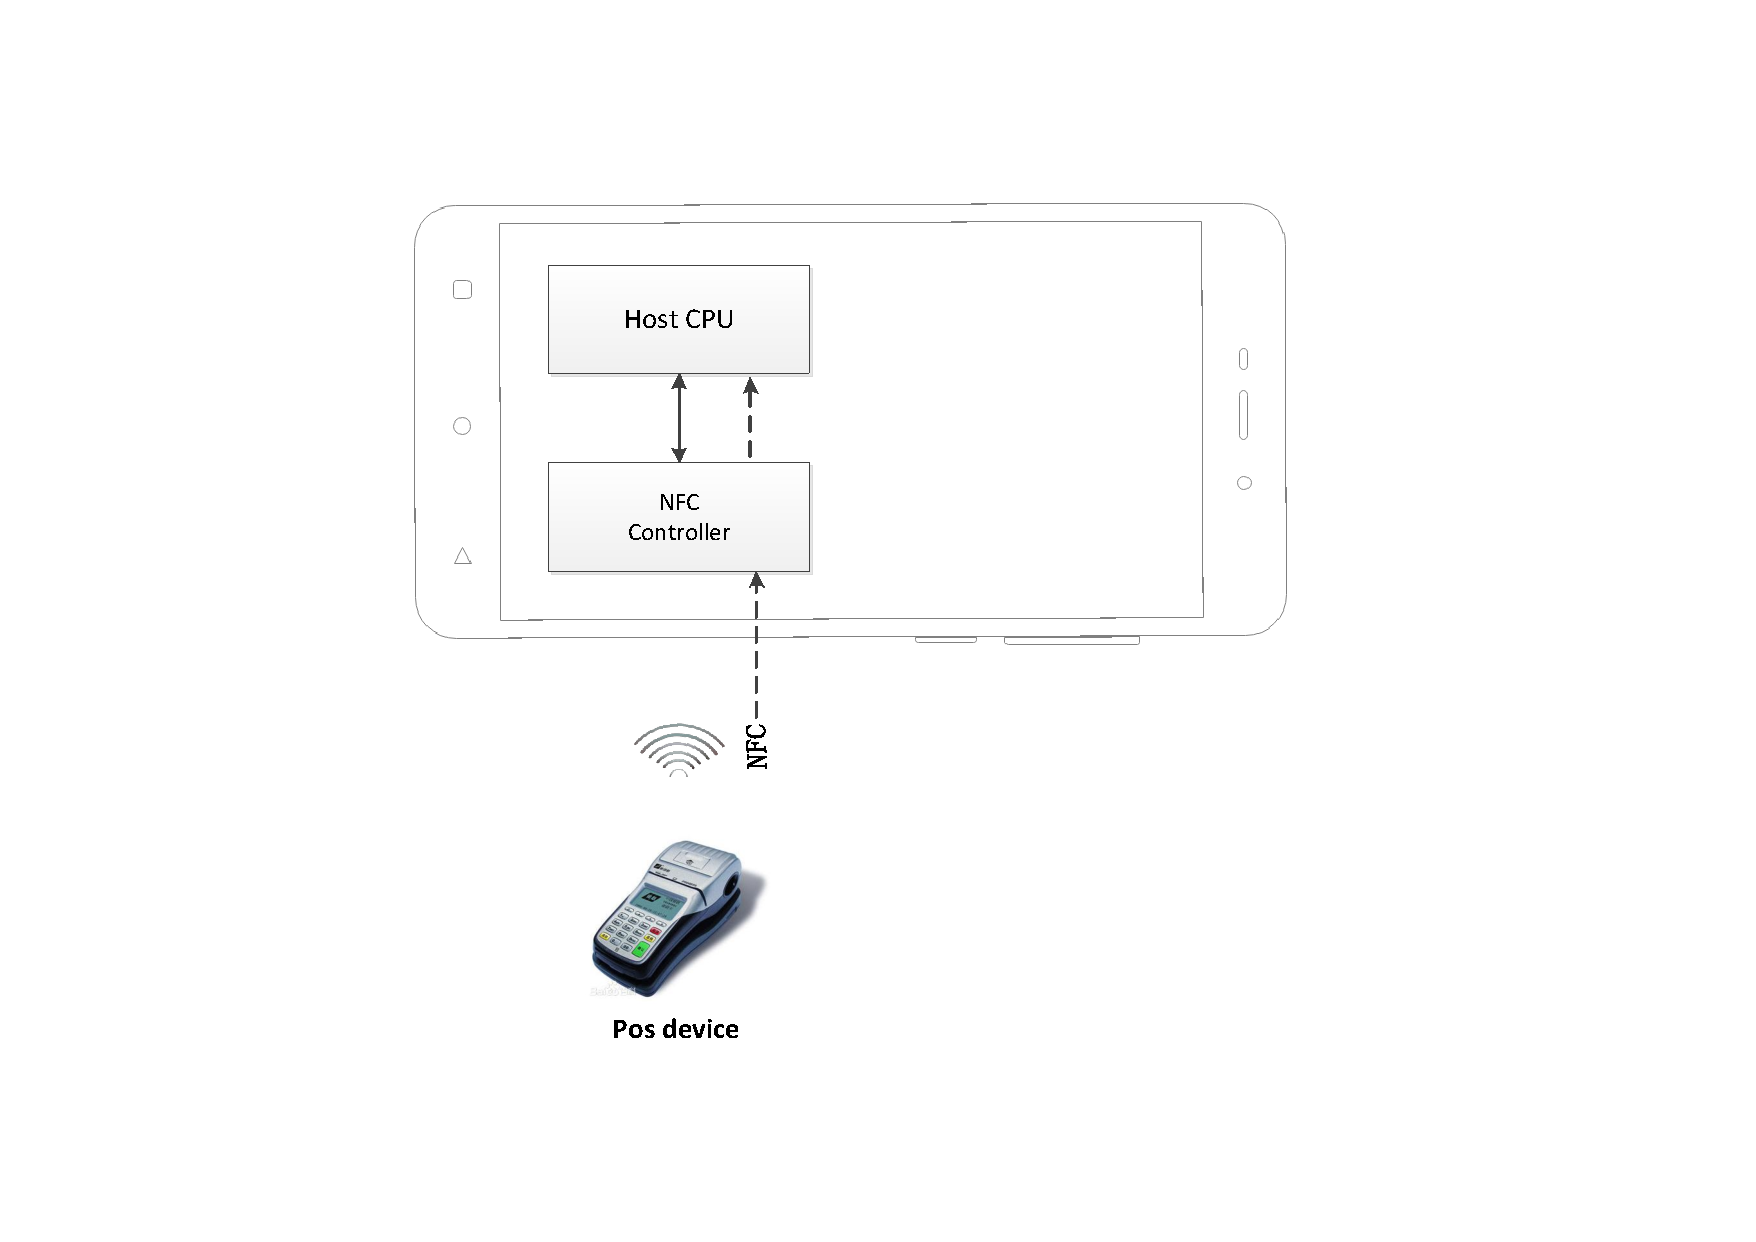
\includegraphics[scale=0.58]{NFC_cpu.pdf}}
\caption{NFC card emulation without a secure element.}
\label{fig}
\end{figure}

\subsection{apple pay}
Apple pays only NFC payments, and its technology is very similar to Samsung's NFC technology, but Apple's use of the scene is not Samsung. Because it does not support magnetic stripe payments, it supports Apple payments on many older devices that only support magnetic stripe payments.

By comparison, it is not difficult to see that Apple Pay and Samsung Pay have an essential difference from China’s Alipay/WeChat. Apple Pay and Samsung Pay do not have their own account ecology. They are only used to replace bank cards for online and offline consumption, eliminating the need to carry bank cards or memories, but are limited to only supporting their own models, and their audiences are relatively Narrower.

Apple's core technology is still Tokenization. Not only that, Apple is also one of the promoters of the Payment Token specification.Although almost all foreign or domestic analysis articles have intentionally or unintentionally mentioned that Apple Pay has implemented the EMVCo specification, so far no official information from Apple or EMVCo has mentioned that Apple Pay has implemented the Tokenisation specification of EMVCo, but The process of adding a card to Apple Pay is very similar to that of EMVCo's request token. At this time, Apple plays the role of a “token requester” (the specification of EMVCo explicitly mentions that the device manufacturer that makes mobile payment can be One of the main categories of token requestors), the bank or payment network plays the role of a token service provider. In addition, the dynamic security code that provides basic security for Apple Pay transactions is very similar to the method of generating and using the Token Cryptogram of the EMVCo specification. Rethinking that Visa and MasterCard have disclosed their tokenization services after the launch of Apple Pay, we have reason to believe that Apple Pay actually implements the Tokenisation specification of EMVCo.

Like the Samsung, the ios system has an application called wallet. When you bind a card, you need to connect to an Apple Pay server.Similarly, the Apple Pay server will also request the virtual bank card from the bank or card organization server with the bank card information submitted by the user.

The mobile phone and Apple Pay server do not save the full bank card number, and only store the unique Device Account Number in the SE. (The payment credentials generated by DAN's iPhone device information and Token encryption can effectively prevent the leakage of credit card information.

Apple Pay is a product that integrates various technologies and resources. Its composition is more complex. The core components include:



\textbf{Secure Element:} The short name SE, which is often referred to as a security element, is an electronic component that resists physical attacks. It contains a microprocessor, storage, and encryption/decryption hardware. It can be used independently (for example, a chip card) or embedded in other devices. Medium (eg, Apple Pay and Google Wallet) provide high security services. Apple Pay uses the form of eSE. Specifically, Apple Pay uses industry standards. A secure element that is compatible with the electronic trading requirements of the financial industry by running the Java Card Platform (JCP). SE is the core of Apple Pay security. In essence, all payment processing and security related to Apple Pay are under the responsibility of SE. Other components only play a supporting role.

The SE(Secure Element) technology is based on the Secure Element specification released by the GlobalPlatform organization. The GlobalPlatform organization is an international standards organization that develops security chip technology standards. Important members include ARM, AMD, AT\&T, China Mobile, VISA, Apple, Samsung, Huawei, etc.

Secure Element is a GP card specification compliant Java card that can contain multiple security domains corresponding to different issuing banks or payment network entities. These security domains are shared with corresponding management parties for verifying identity and secure communication of management parties. The key. Personalized data from card issuing banks or payment networks, encrypted using these shared keys, can be securely distributed to the corresponding security domain, thus completing the personalization process for payment of Applet, which is the same as traditional payment card personals. The process is similar
    
    \textbf{NFC controller:} NFC controller. In the context of Apple Pay, the NFC controller acts as a router. It is connected to three different external entities: external near-field devices (eg, point-of-sale (POS), point-of-sale), and applications. The processor (AP, Application Processor) and Secure Element, in turn, form two communication channels: the application processor's communication channel to the Secure Element, and the communication channel between the POS and the Secure Element.
    
    \textbf{Wallet:}The Wallet was originally called the passbook and was renamed wallet after IOS 9. It was a service that existed before the Apple Pay product was released. After Apple Pay was released, Apple expanded its functionality to allow it to add and manage credit cards and debit cards for Apple Pay.Of course, It can also check the added card information, the bank's privacy policy, and recent transaction details. For Apple Pay, Wallet is equivalent to the management client of Secure Element. Adding or deleting card or debit card information in Secure Element can be performed via the Wallet service.
   
    \textbf{Touch ID:} This is the iPhone's fingerprint recognition service. Its purpose is to use fingerprint recognition to make access to the device more secure, faster, and easier. Touch ID is not a replacement of the device security password, but allows users to use complex device passwords without sacrificing convenience. In other words, users can use complex passwords to protect the device while also using the Touch ID to easily access the device.
   
    \textbf{Secure Enclave:} Secure Enclave is an internal secure execution environment for iOS devices. It can be used to process sensitive information. For example, the data acquired by Touch ID's fingerprint imaging sensor needs to be passed to Secure Enclave for the actual fingerprinting process. For Apple Pay, Secure Element manages the certification process and makes payment transactions possible.
    Secure Enclave is a coprocessor packaged together by the Apple A7 and subsequent series of application processors. It has its own secure boot process and personalized software update process, and it is separate from the application processor where the iOS system is located. Secure Enclave uses encryption (using a temporary generated key encryption) physical memory (a portion of the physical memory shared by the application processor) for business processing and has its own hardware random number generator. Secure Enclave communicates with the application processor through the interrupt-driven mailbox and shared memory, and provides all cryptographic services related to data protection key management.

The ARM TrustZone technology we are familiar with is essentially a virtualization technology that divides processor state into secure and non-secure states, and cooperates with other buses and security attributes on peripherals to achieve security throughout the entire hardware system. Like Secure Enclave, ARM TrustZone has its own secure boot process and personalized software update process. It also has its own hardware random number generator (and other similar security peripherals), and is also driven by the interrupt between the same application processor. Monitor mode and shared memory for communication. It can be seen that the security features provided by Secure Enclave have not exceeded the scope of ARM TrustZone technology.


Apple has never mentioned that Secure Enclave is an implementation of the ARM TrustZone security extension technology (although according to the description of several secure communication channels in the official Apple documentation, Secure Enclave is probably an implementation of the ARM TrustZone technology), we are still It is impossible to determine whether the Secure Enclave is an independent coprocessor or an application processor running state (both architectures can provide the required security features of Secure Enclave), this needs to be announced by Apple for more details of the implementation of Secure Enclave, At present, it can be concluded that the security features provided by Secure Enclave can also be implemented

\textit{1) Communication security between Secure Enclave and Touch ID:}We know that the fingerprint data acquired by the Touch ID imaging array needs to be actually matched by the Secure Enclave. In the implementation of Apple Pay, the Touch ID sensor is connected to the application processor through the serial peripheral interface bus (Serial Peripheral Interface Bus). Connect and then connect to the Secure Enclave. In other words, the fingerprint imaging data acquired by the fingerprint sensor needs to be relayed via the application processor. This poses a security risk: malicious programs can intercept the data generated by the Touch ID sensor. Apple Pay realizes the secure transmission of fingerprint data in a simple way. First, the Touch ID sensor and Secure Enclave will preset a shared key, then use the shared key to negotiate a session key, and then use the negotiated session key to use. The AES-CCM algorithm encrypts the transmitted data. This ensures that the application processor cannot read fingerprint data and ensures the security of the entire fingerprinting process.
    
\textit{2) Communication security between Secure Enclave and Secure Element: }  
As mentioned earlier when the NFC controller was introduced, the physical communication channel between the Secure Enclave and the Secure Element needs to be relayed through the NFC controller. There is no direct physical connection between the two, which is specifically the Secure Element and NFC controller. Connected, and then the NFC controller is connected to the application processor without mentioning how the NFC controller is connected to the Secure Enclave (as stated by Apple's official documentation, it can be seen here that the Secure Enclave is probably not a separate coprocessor), Then, since Secure Element and Secure Enclave need to transit through the application processor, it is necessary to consider the communication security.

The implementation is similar to the process of communicating with Touch ID and Secure Enclave. It also encrypts the communication content by sharing the pairing key. However, because the Secure Element is involved, the preset of the shared pairing key is more complicated, specifically: The pairing key is preset at the production stage, and the key is generated by the Secure Enclave using its own UID key and the unique identifier of the Secure Element as input, and then securely transmitted to the external hardware security module (HSM, Hardware) in the factory. Security Module) and then injected into Secure Element. In actual use, the communication between Secure Element and Secure Enclave is encrypted using an AES-based cryptographic algorithm, and a cryptographic mechanism is used to prevent replay attacks.


\begin{figure}[htbp]
\centerline{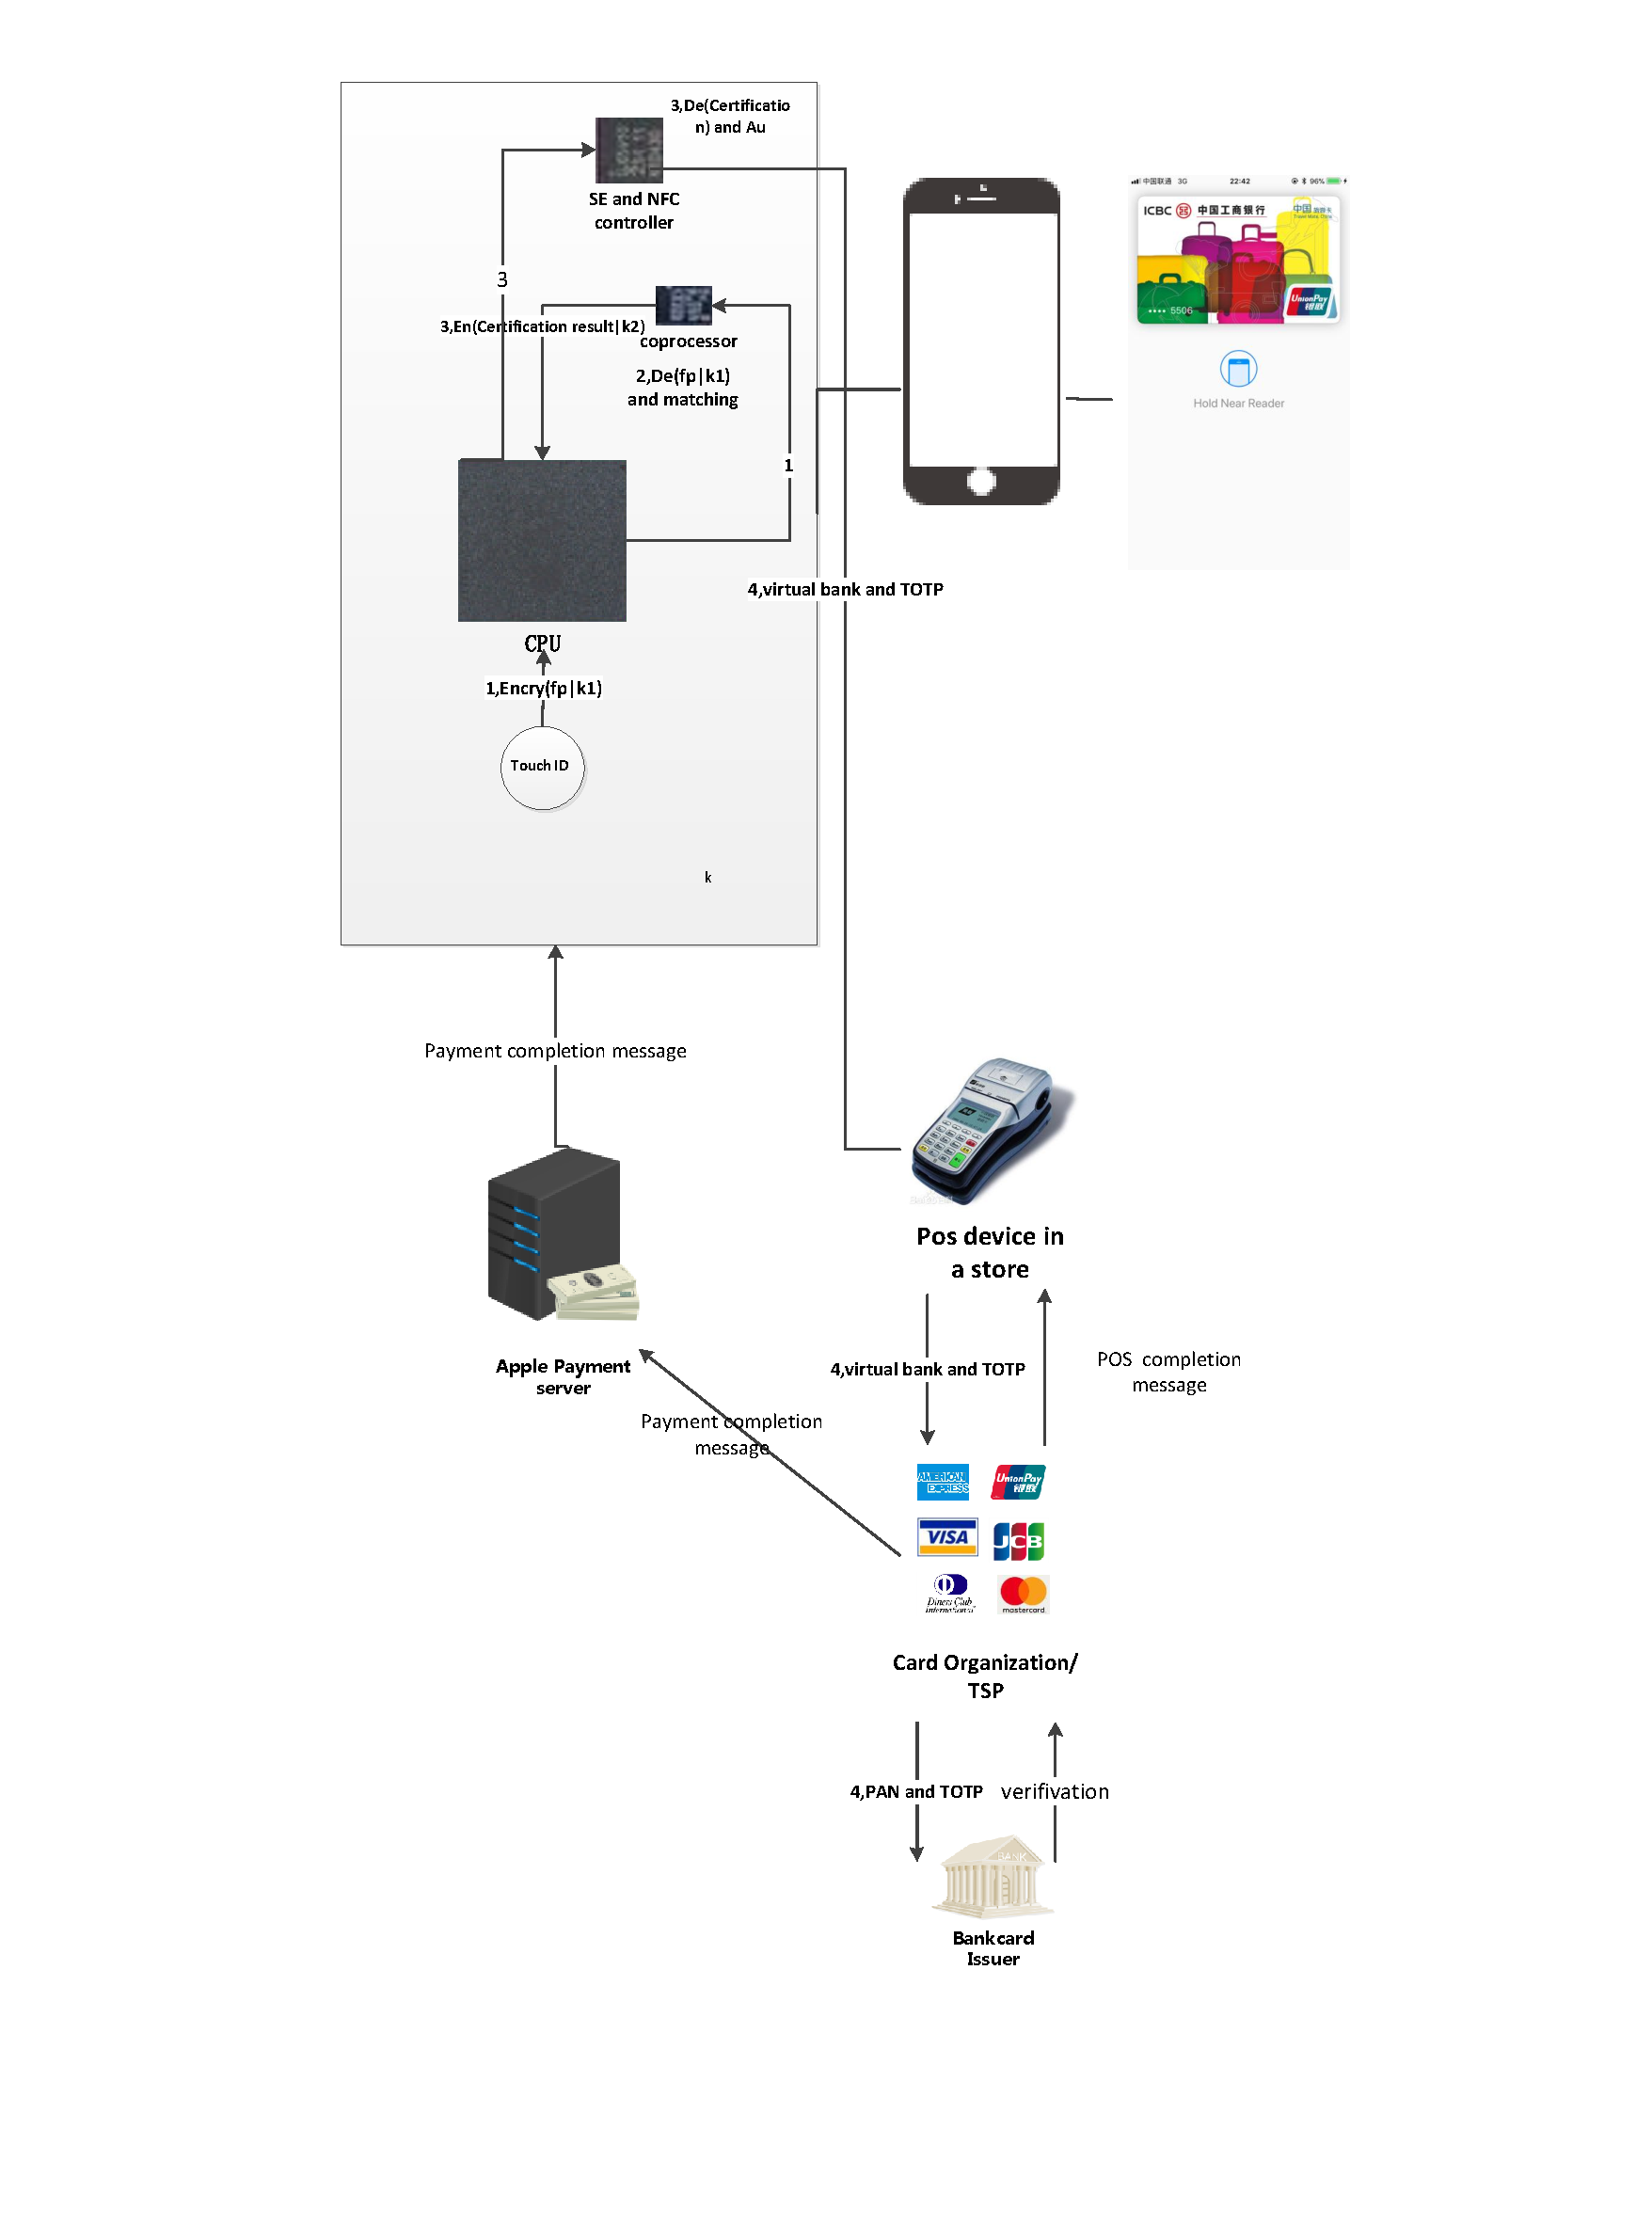
\includegraphics[scale=0.5]{iphone_pay.pdf}}
\caption{Iphone security payment.}
\label{fig}
\end{figure}
    
    \textbf{Apple Pay Servers:} Apple Pay Server, which manages the status of credit and debit cards in Passbooks as well as device-specific account information stored in Secure Element. The Apple Pay server communicates with both the device and the server in the Payment Network. For in-app payments, the Apple Pay server is also responsible for using merchant-specific keys and Payment Credentials for Apple Pay. Encrypt it and send it to the actual merchant server for payment processing.

 using ARM TrustZone technology.

\begin{figure}[htbp]
\centerline{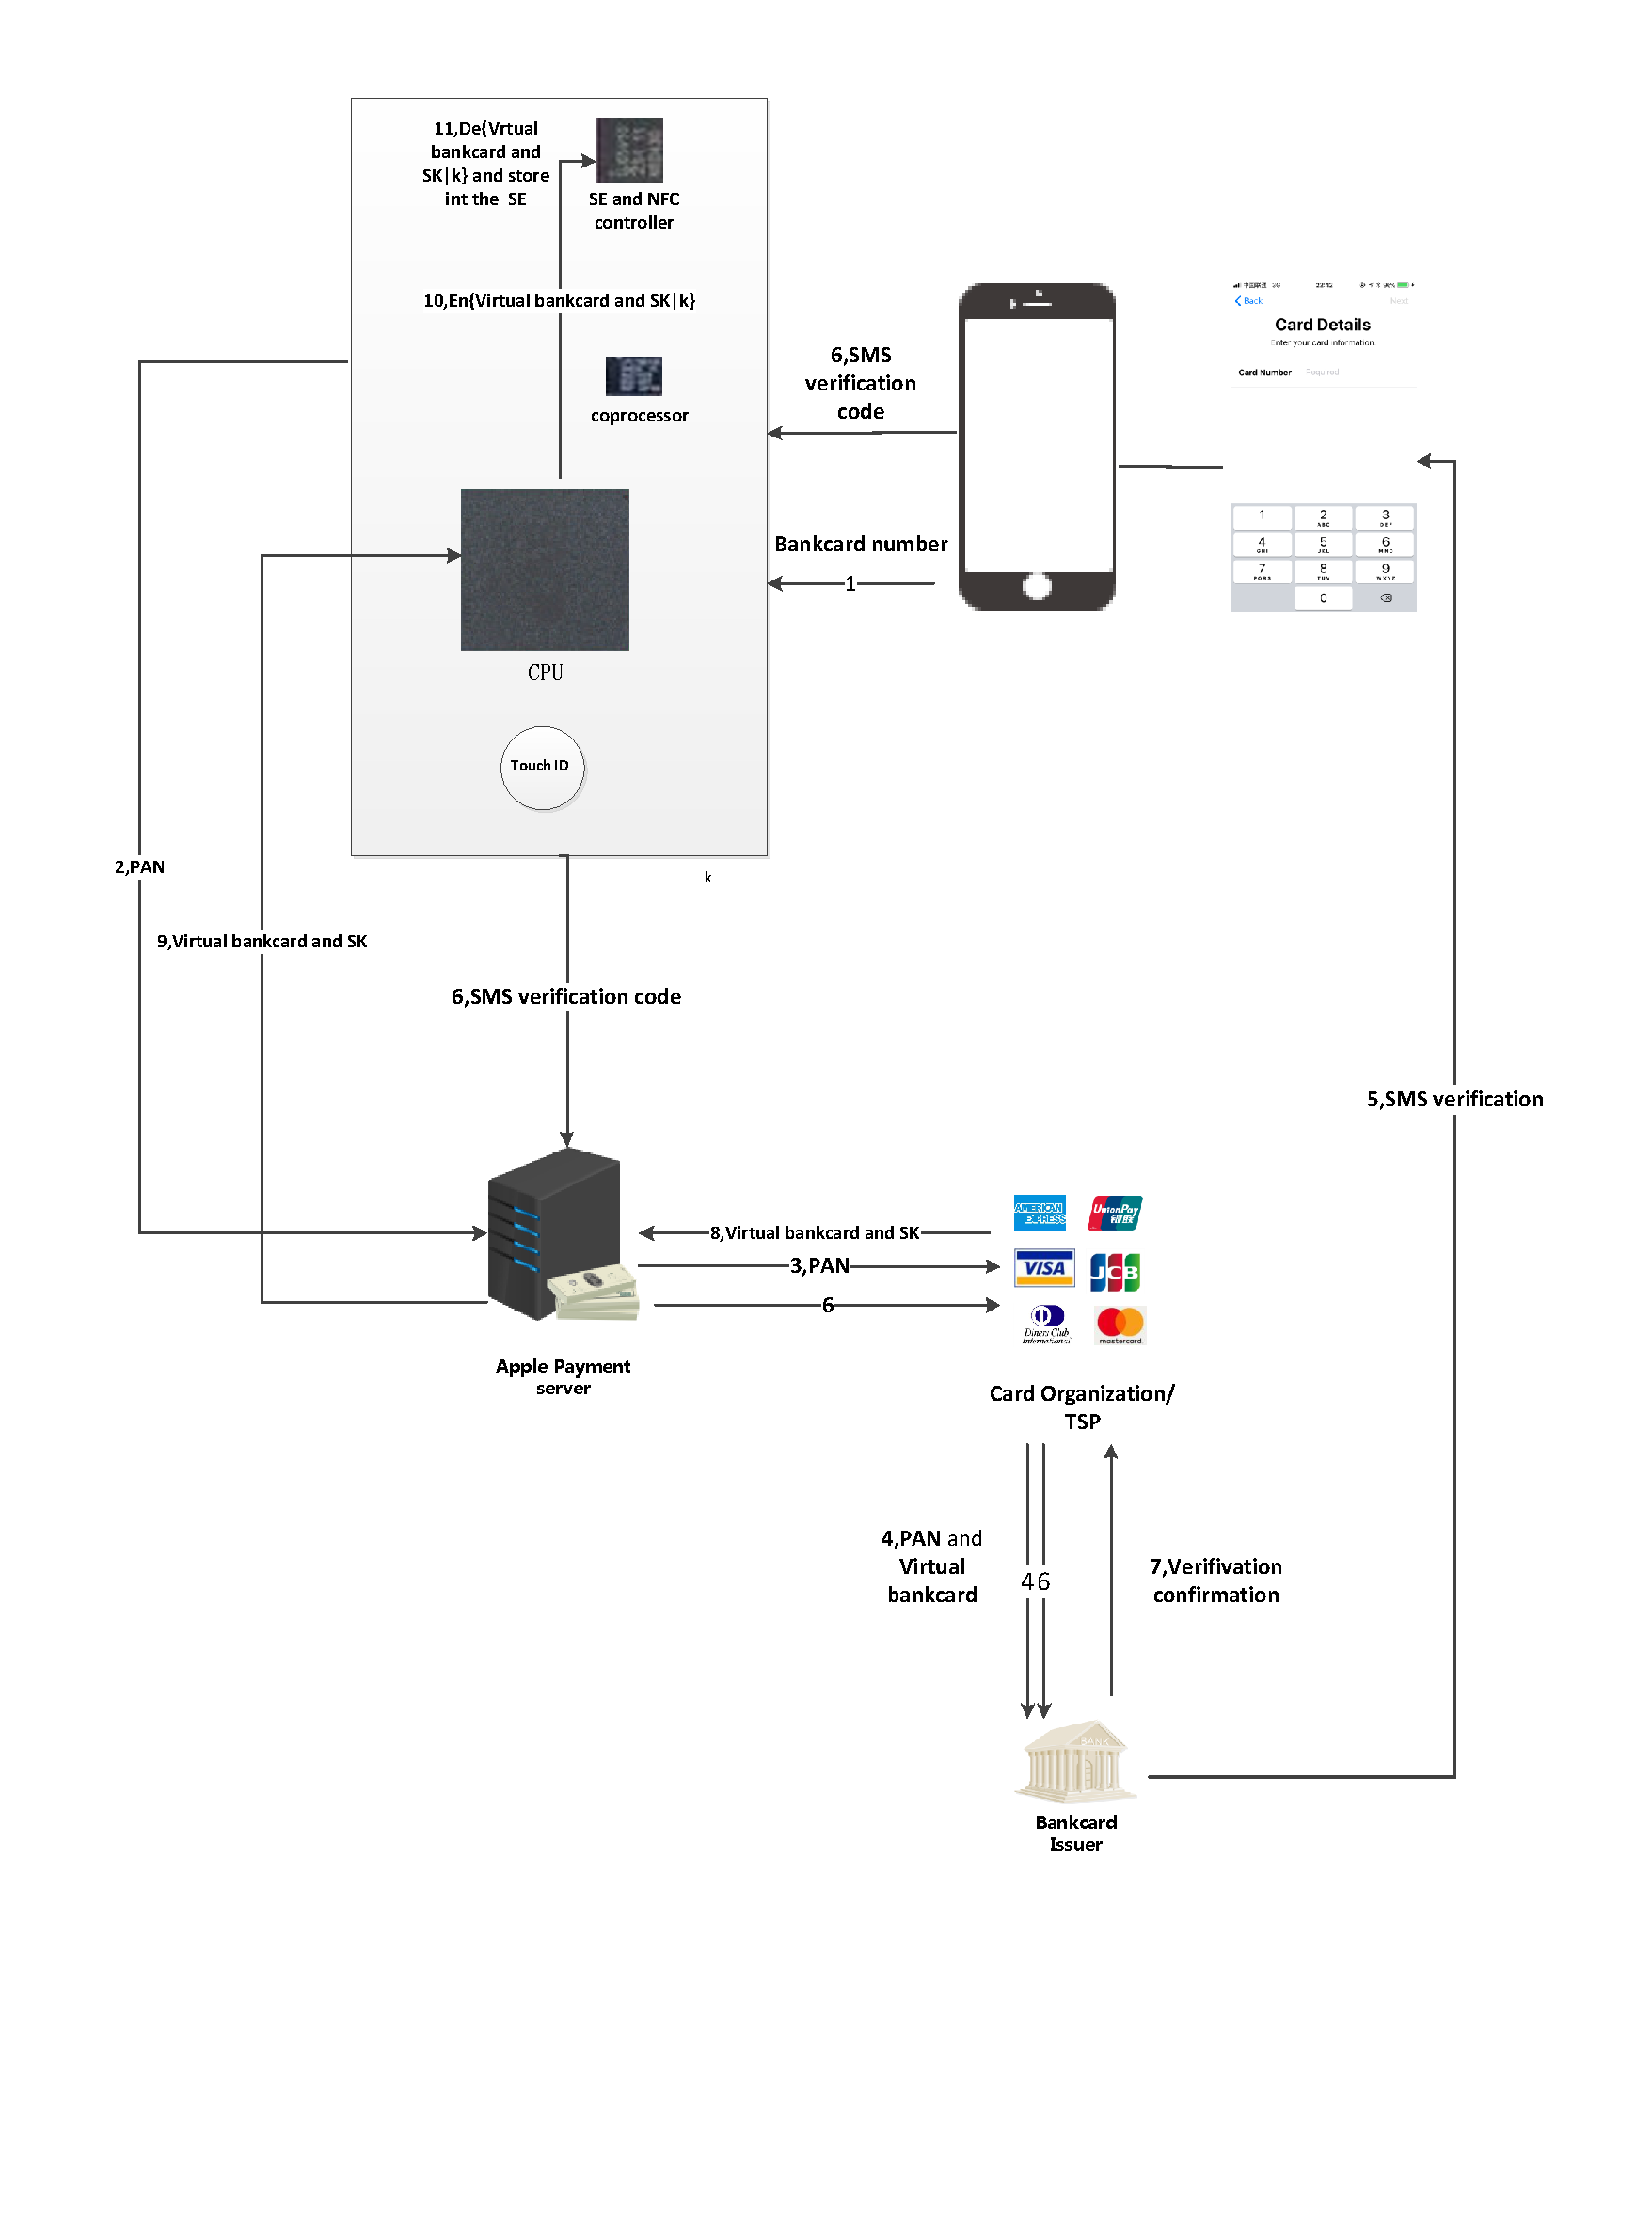
\includegraphics[scale=0.37]{iphone_tsp.pdf}}
\caption{Iphone security payment component.}
\label{fig}
\end{figure}

\section{Disscusion and security comparison}
\begin{figure*}[htbp]
\centerline{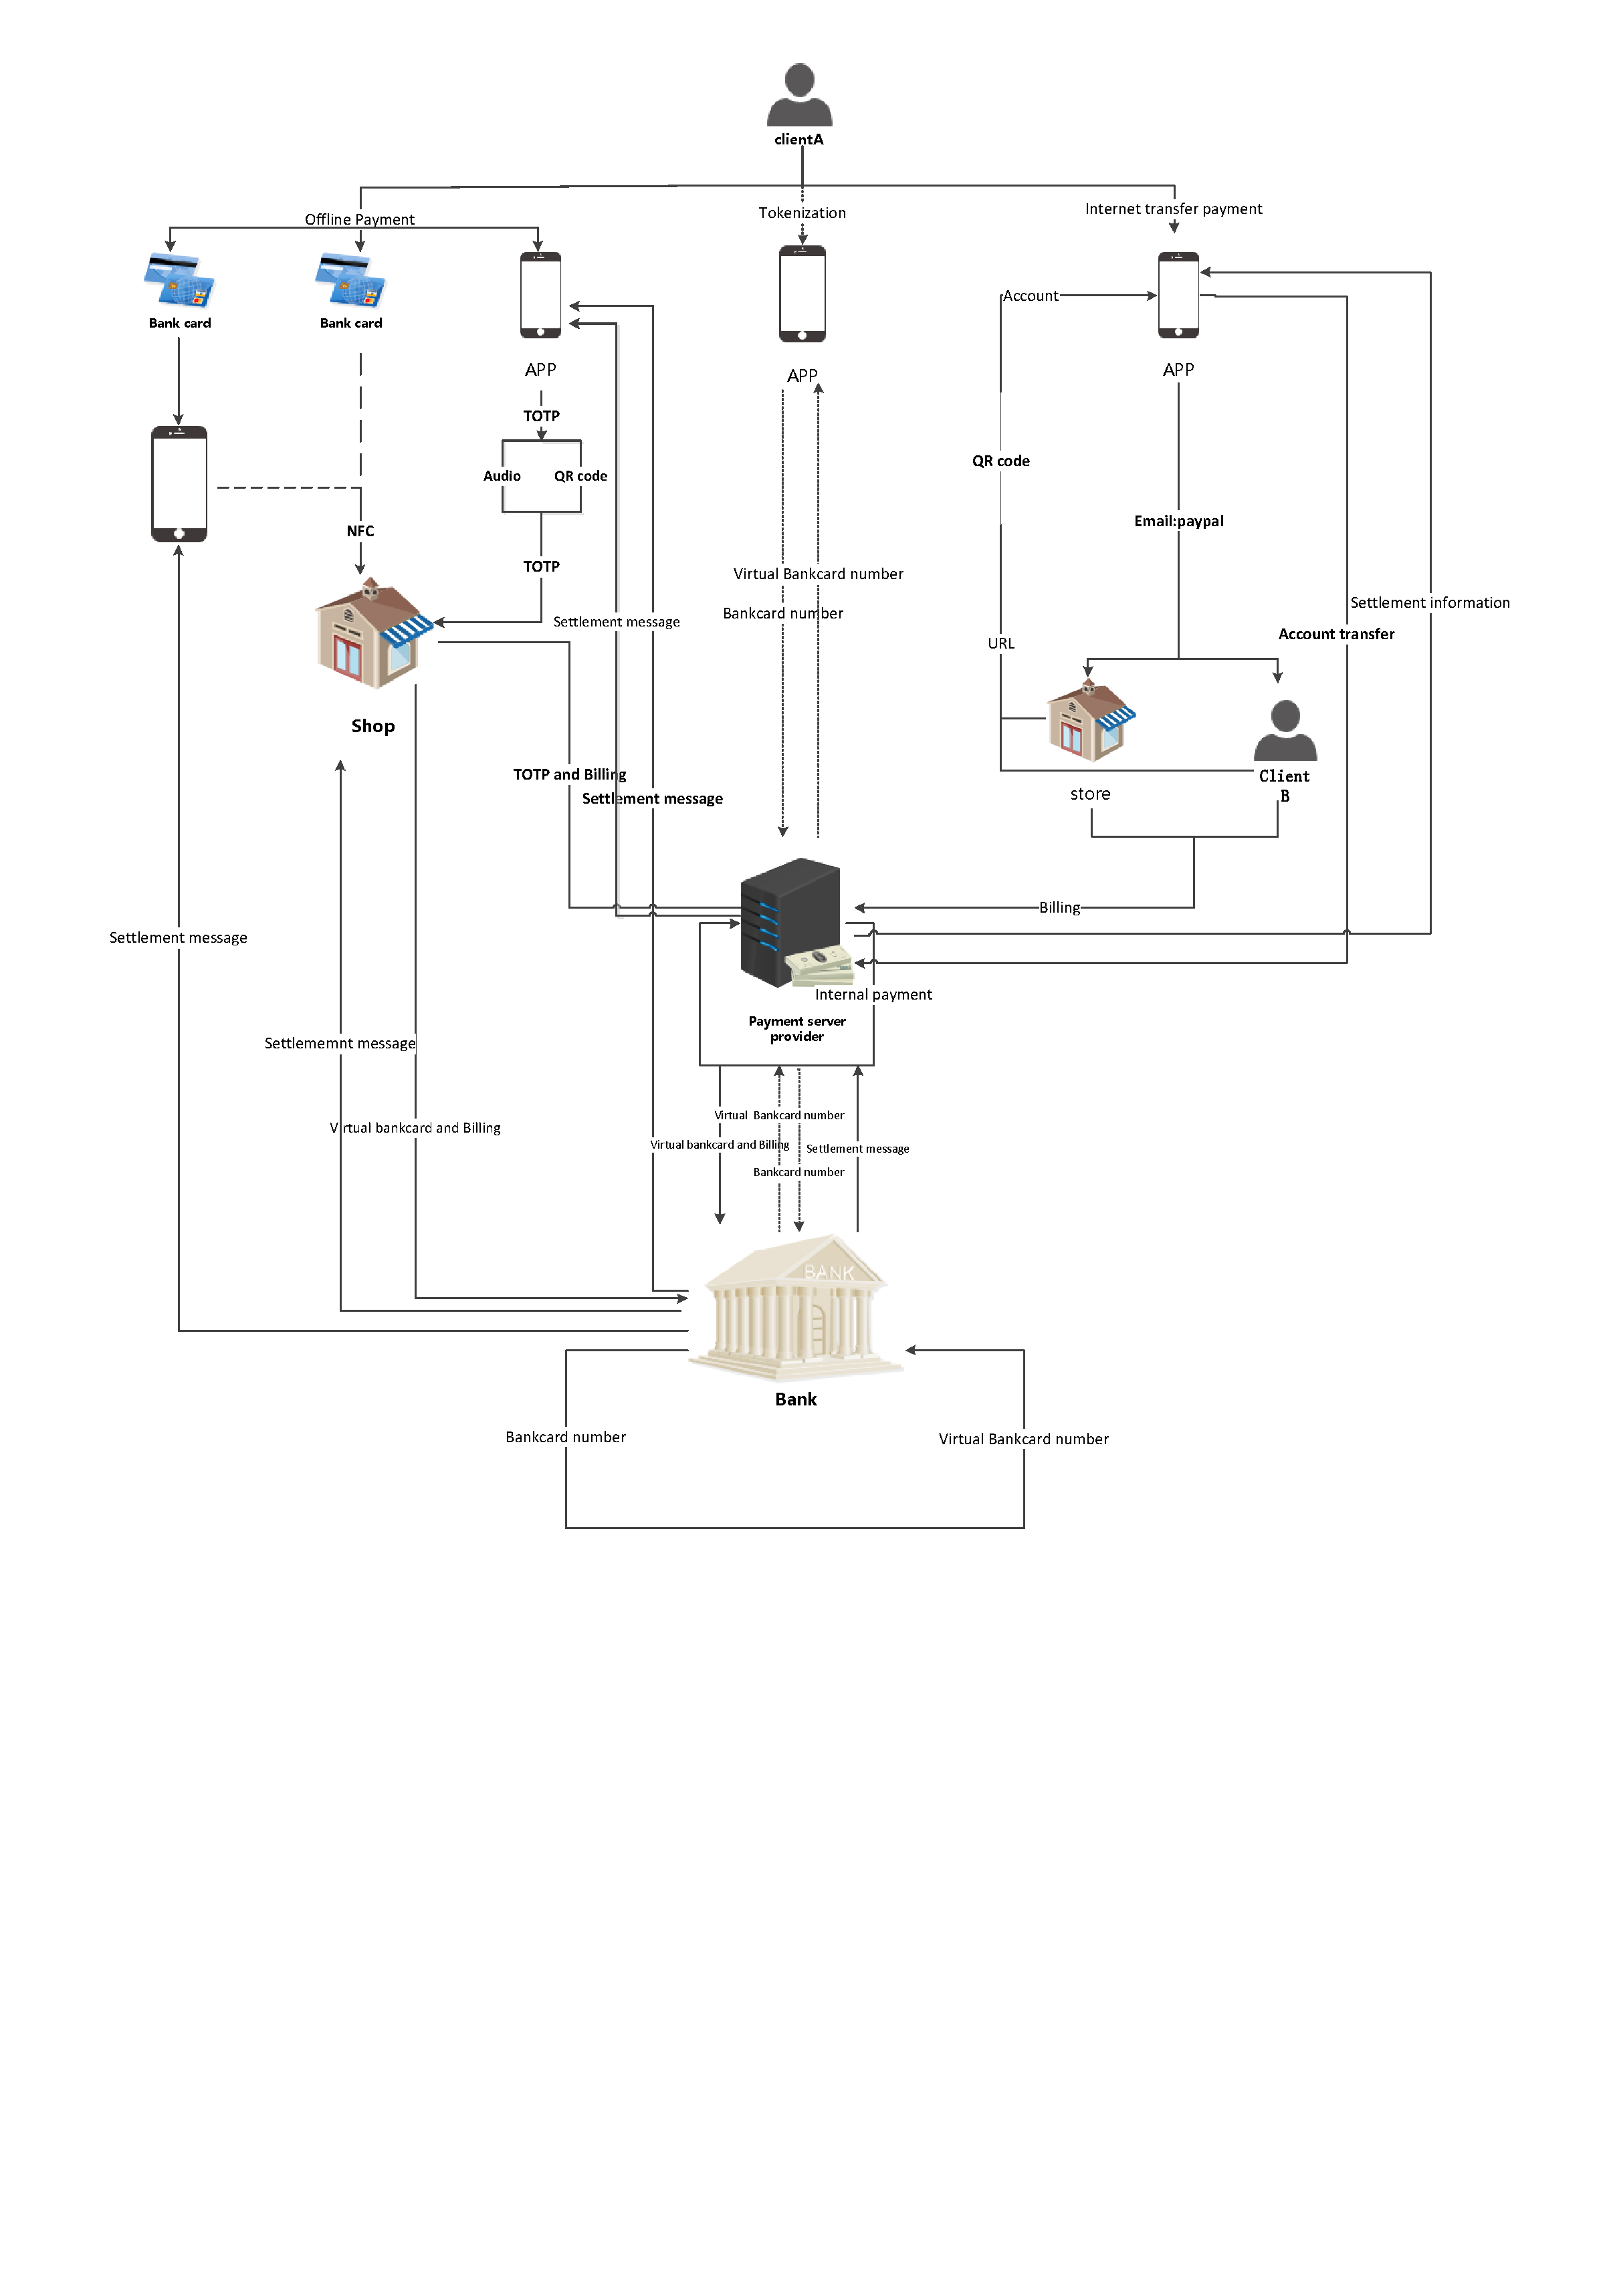
\includegraphics[scale=0.5]{datu.pdf}}
\caption{Time-Based One-Time Password.}
\label{fig}
\end{figure*}


\section{Conclusion}
The conclusion goes here.





% if have a single appendix:
%\appendix[Proof of the Zonklar Equations]
% or
%\appendix  % for no appendix heading
% do not use \section anymore after \appendix, only \section*
% is possibly needed

% use appendices with more than one appendix
% then use \section to start each appendix
% you must declare a \section before using any
% \subsection or using \label (\appendices by itself
% starts a section numbered zero.)
%


\appendices
\section{Proof of the First Zonklar Equation}
Appendix one text goes here.

% you can choose not to have a title for an appendix
% if you want by leaving the argument blank
\section{}
Appendix two text goes here.


% use section* for acknowledgment
\section*{Acknowledgment}


The authors would like to thank...


% Can use something like this to put references on a page
% by themselves when using endfloat and the captionsoff option.
\ifCLASSOPTIONcaptionsoff
  \newpage
\fi



% trigger a \newpage just before the given reference
% number - used to balance the columns on the last page
% adjust value as needed - may need to be readjusted if
% the document is modified later
%\IEEEtriggeratref{8}
% The "triggered" command can be changed if desired:
%\IEEEtriggercmd{\enlargethispage{-5in}}

% references section

% can use a bibliography generated by BibTeX as a .bbl file
% BibTeX documentation can be easily obtained at:
% http://mirror.ctan.org/biblio/bibtex/contrib/doc/
% The IEEEtran BibTeX style support page is at:
% http://www.michaelshell.org/tex/ieeetran/bibtex/
%\bibliographystyle{IEEEtran}
% argument is your BibTeX string definitions and bibliography database(s)
%\bibliography{IEEEabrv,../bib/paper}
%
% <OR> manually copy in the resultant .bbl file
% set second argument of \begin to the number of references
% (used to reserve space for the reference number labels box)
\begin{thebibliography}{1}

\bibitem{IEEEhowto:kopka}
H.~Kopka and P.~W. Daly, \emph{A Guide to \LaTeX}, 3rd~ed.\hskip 1em plus
  0.5em minus 0.4em\relax Harlow, England: Addison-Wesley, 1999.
 
\bibitem{IEEEhowto:kopka}
Agbinya J I, Masihpour M. \emph{Power Equations and Capacity Performance of Magnetic Induction Communication Systems[J]}. Wireless Personal Communications, 2012, 64(4):831-845.
\bibitem{IEEEhowto:kopka}
Timalsina S K, Moh S. A review on NFC and NFC-based mobile payment solution[J]. Journal of Next Generation Information Technology, 2012, 3(4):35-44.
\bibitem{IEEEhowto:kopka}
NFC Forum, “\emph{White paper on ’smart posters’},” Tech. Rep., Apr. 2011.
\bibitem{IEEEhowto:kopka}
NFC Forum, \emph{“White paper on ’essentials for successful NFC mobile ecosystem’,}” Tech. Rep., Oct.
2008.
\bibitem{IEEEhowto:kopka}
NFC Forum, \emph{“White paper on ’the keys to truly interoperable communications’},” Tech. Rep., Oct.2007.
\bibitem{IEEEhowto:kopka}
R. Steffen, J. Prei andinger, T. Scho andllermann, A. Mu andller, and I. Schnabel, \emph{“Near field communication (NFC) in an automotive environment,}” Proc. of 2010 Second International Workshop on Near Field Communication (NFC), pp. 15-20, Apr. 2010.
\bibitem{IEEEhowto:kopka}
E. Haselsteiner and K. Breitfu, \emph{“Security in near field communication (NFC),}” Proc. of Workshop on RFID security, 2006.
\bibitem{IEEEhowto:kopka}
E. Haselsteiner and K. Breitfu, \emph{“Security in near field communication (NFC),}” Proc. of Workshop
on RFID security, 2006.
\bibitem{IEEEhowto:kopka}
PCI Security Standards Council. Information supplement: PCI DSS tokenization guidelines, 2011. Available at "\url{https:www.pcisecuritystandards.org/documents/Tokenization_Guidelines_Info_Supplement.pdf}".
\bibitem{IEEEhowto:kopka}
Díaz-Santiago, S., Rodriguez-Henriquez, L. M., \& Chakraborty, D. (2016). \emph{A cryptographic study of tokenization systems.} International Conference on Security and Cryptography (Vol.15, pp.413-432). IEEE.
\bibitem{IEEEhowto:kopka}
E. Haselsteiner and K. Breitfu, \emph{“Security in near field communication (NFC),”} Proc. of Workshop on RFID security, 2006.
\bibitem{IEEEhowto:kopka}
C. Mulliner, \emph{“Vulnerability analysis and attacks on NFC-enabled mobile phones,”} Proc. of International Conference on Availability, Reliability and Security (ARES ’09), pp. 695-700, Mar.2009.
\bibitem{IEEEhowto:kopka}
Timalsina S K, Moh S. \emph{A review on NFC and NFC-based mobile payment solution[J]}. Journal of Next Generation Information Technology, 2012, 3(4):35-44.
\bibitem{IEEEhowto:kopka}
Alves T. \emph{TrustZone : Integrated Hardware and Software Security[J]. White Paper}, 2004.
\bibitem{IEEEhowto:kopka}
Kanniainen L. \emph{Alternatives for banks to offer secure mobile payments[J]}. International Journal of Bank Marketing, 2010, 28(5):433-444.
\bibitem{IEEEhowto:kopka}
Coskun V, Ozdenizci B, Ok K. \emph{A Survey on Near Field Communication (NFC) Technology[J]}. Wireless Personal Communications, 2013, 71(3):2259-2294.
\bibitem{IEEEhowto:kopka}
Reveilhac M, Pasquet M. \emph{Promising Secure Element Alternatives for NFC Technology[C]}.International Workshop on Near Field Communication. IEEE, 2009:75-80.
\bibitem{IEEEhowto:kopka}
Micro Focus, \emph{Secure Stateless Tokenization (SST)}, Available at "\url{http://files.asset.microfocus.com/4aa6-5576/en/4aa6-5576.pdf}".
\bibitem{IEEEhowto:kopka}
Terence Spies, Mountain View, CA(US),Richard T.Minner, Carmichael, CA(US), \emph{system for protecting sensitive data with distributed tokenization}, US 8595850 B2, 2013-11-26.
\bibitem{IEEEhowto:kopka}
Ulf Mattsson, Stamford, CT(US), \emph{distributed tokenization using several substitution steps}, US 8745094 B2, 2014-6-3.
\bibitem{IEEEhowto:kopka}
Ulf Mattsson, Cos Cob,CT(US), Yigal Rozenberg, Wilton, CT(US),Vichai Levy, Norwalk, CT(US), \emph{table-connected tokenization}, US 9237006 B2, 2016-1-12. 
\bibitem{IEEEhowto:kopka}
Nojiri T. \emph{Two-dimensional code, methods and apparatuses for generating, displaying and reading the same}: US, US 7032823 B2[P]. 2006.
\bibitem{IEEEhowto:kopka}
Hara M, Watabe M. \emph{Two dimensional code reading apparatus}: EP, US 5691527 A[P]. 1997.
\bibitem{IEEEhowto:kopka}
Hara, Masahiro, Watabe, Motoaki, Nojiri, Tadao , Nagaya, Takayuki, Uchiyama, Yuji.\emph{Optically readable two-dimensional code and method and apparatus using the same}:US 5726435. 1995.
\bibitem{IEEEhowto:kopka}
Coskun V, Ozdenizci B, Ok K. \emph{A Survey on Near Field Communication (NFC) Technology[M]}. Kluwer Academic Publishers, 2013.
\bibitem{IEEEhowto:kopka}
Vedat Coskun, Busra Ozdenizci, Kerem Ok. \emph{The Survey on Near Field Communication[J]}. 2015, 15(6):13348-13405.
\bibitem{IEEEhowto:kopka}
Brown, T.W.C.; Diakos, T. \emph{On the Design of NFC Antennas for Contactless Payment Applications}. In Proceedings of the 5th European Conference on Antennas and Propagation (EUCAP), Rome, Italy, 11–15 April 2011; pp. 44–47.
\bibitem{IEEEhowto:kopka}
Gebhart, M.; Szoncso, R. O\emph{ptimizing Design of Smaller Antennas for Proximity Transponders}.
In Proceedings of the IEEE Second International Workshop on Near Field Communication,
Monaco, 20 April 2010; pp. 77–82.
\bibitem{IEEEhowto:kopka}
Coskun V, Ozdenizci B, Ok K. \emph{A Survey on Near Field Communication (NFC) Technology[J]}. Wireless Personal Communications, 2013, 71(3):2259-2294.
\bibitem{IEEEhowto:kopka}
Coskun V, Ok K, Ozdenizci B. \emph{Near Field Communication (NFC): From Theory to Practice[J]}. 2012, 13(March 10):816-825.

\bibitem{IEEEhowto:kopka}
Roland M, Langer J. D, \emph{igital Signature Records for the NFC Data Exchange Format[C]// Second International Workshop on Near Field Communication}. IEEE, 2010:71-76.
\bibitem{IEEEhowto:kopka}
Aziza H. \emph{NFC Technology in Mobile Phone Next-Generation Services[C]}, Second International Workshop on Near Field Communication. IEEE Computer Society, 2010:21-26.
\bibitem{IEEEhowto:kopka}
Luca G D, Lillo P, Mainetti L, et al. \emph{The use of NFC and Android technologies to enable a KNX-based smart home[C]}, International Conference on Software, Telecommunications and Computer Networks. IEEE, 2013:1-7.

\bibitem{IEEEhowto:kopka}
Coskun V, Ok K, Ozdenizci B. \emph{Professional NFC Application Development for Android[M]}. Wiley, 2013.
\bibitem{IEEEhowto:kopka}
Plos T, Hutter M, Cavaliere F, et al. \emph{Security-Enabled Near-Field Communication Tag With Flexible Architecture Supporting Asymmetric Cryptography[J]}. IEEE Transactions on Very Large Scale Integration Systems, 2013, 21(11):1965-1974.


\end{thebibliography}


% biography section
% 
% If you have an EPS/PDF photo (graphicx package needed) extra braces are
% needed around the contents of the optional argument to biography to prevent
% the LaTeX parser from getting confused when it sees the complicated
% \includegraphics command within an optional argument. (You could create
% your own custom macro containing the \includegraphics command to make things
% simpler here.)
%\begin{IEEEbiography}[{\includegraphics[width=1in,height=1.25in,clip,keepaspectratio]{mshell}}]{Michael Shell}
% or if you just want to reserve a space for a photo:

\begin{IEEEbiography}{Michael Shell}
Biography text here.
\end{IEEEbiography}

% if you will not have a photo at all:
\begin{IEEEbiographynophoto}{John Doe}
Biography text here.
\end{IEEEbiographynophoto}

% insert where needed to balance the two columns on the last page with
% biographies
%\newpage

\begin{IEEEbiographynophoto}{Jane Doe}
Biography text here.
\end{IEEEbiographynophoto}


% You can push biographies down or up by placing
% a \vfill before or after them. The appropriate
% use of \vfill depends on what kind of text is
% on the last page and whether or not the columns
% are being equalized.

%\vfill

% Can be used to pull up biographies so that the bottom of the last one
% is flush with the other column.
%\enlargethispage{-5in}



% that's all folks
\end{document}


